\input{preamble}

\begin{document}

\begin{flushright}
Laura Fields\\
Paul Lebrun \\
Seongtae Park \\
Amit Bashyal \\
Blake Watson \\
\today
\end{flushright}

%title
\begin{center}

{\LARGE LBNE Beam Alignment Tolerances and Systematic Uncertainties}
\end{center}

%\tableofcontents

%\begin{abstract} 	

%\end{abstract}

This note describes a study of beam alignment tolerances and systematic uncertainties that was conducted in the winter of 2013-2014.  For each beam alignment parameter listed in Table~\ref{tab:syslist}, we evaluate the systematic uncertainty on the unoscillated muon neutrino flux assuming the nominal tolerances listed in Table~\ref{tab:syslist}.  In addition to providing a preliminary estimate of uncertainties that can be input to physics studies, this work also provides valuable input to the beamline group that will inform the design of hadron monitors and other beam alignment tools.  The note is organized as follows: Section~\ref{sec:beamsim} describes the simulation used to execute the study, the procedure for extracting systematic uncertainties is reviewed in Section~\ref{sec:procedure}, the results are summarized in Section~\ref{sec:results}.  Plots showing the neutrino flux in various beam configurations and the fits used to extract systematic uncertainties are available in Appendices~\ref{app:nof_plots}-~\ref{app:far_plots}

\begin{table}
\centering
\begin{tabular}{ | c | c | }
\hline
  Target position (each end) & 0.5 mm \\
  Horn 1 position (each end) & 0.5 mm \\
  Horn 2 position (each end) & 0.5 mm \\
  Far detector position & 21 m \\
  Decay pipe position & 20 mm \\
  Decay pipe radius & 0.1 m \\
  Horn current & 2 kA \\
  Horn water layer thickness & 0.5 mm \\
  Beam size at target & 0.1 mm \\
  Misalignment of shielding blocks & 1 cm \\
  Baffle scraping & 0.25\% \\
  Beam position at target & 0.45 mm \\
  Beam angle at target & 70 $\mu$rad \\
  Near detector position & 255 mm \\
  Horn conductor skin depth & 6 mm \\
  Target density & 2\% \\ 
\hline
\end{tabular}
\caption{Sources of beam misalignment and their expected tolerances, which were obtained from the LBNE CDR~\cite{lbnecdr} where applicable and from conversations with beam experts otherwise.}
\label{tab:syslist}
\end{table}

\section{Description of Beam Simulation}
\label{sec:beamsim}

This section describes the motivation, goals and scope of the Geant4~\cite{Geant4} application used in the determination of systematics effects for the LBNE   beam line. As the application, named g4lbne-v3, is to a large extend self-describing, this is not a ``user's manual", rather a memo on some technical   aspects of the software. We start by stating the design requirements gathered after producing results with the previous of the software, present   our adopted solution to fix limitations of g4lbne-v2 and comment on some architectural features of the code. 

\subsection{Requirements for  g4lbne-v3}  These requirements were gathered informally during our weekly meeting, over a period of a few weeks, back in April through June 2013. They were:  \begin{enumerate}\item Support the studies of alignments tolerances, particularly for the Horns and the targets.  While the previous version, g4lbne-v2 allowed the users tochange the coordinates of sections of the horns, results were found to be difficult to understand without the confidence that the Geant4 geometry was sound.That is, that both the volumes were set as intended by the user, and the Geant4 tracking was self consistent, with no volume overlap, or other limitations thatwere hard to debug.  While details of the geometrywas set by the ASCII geometry data file, the overall program flow was determined by the Geant4 User Interface (G4UI) data cards, causing occasional confusion. \item Back then, the first phase of LBNE consistent of using the NUMI beamline design, the so-called 700 kW option, including it's horns and target. Detailedengineering drawing were therefore available, allowing us to implement an actual and precise geometry in our simulation. Such a drive for correctness makessense in the context of the study of systematic effects. \item Allow for some optimization of the geometry, to enhance the neutrino flux around both the first and second oscillation peaks, while mitigating the high energy component of the neutrino flux, while preserving the level of details required for correctness. Such an optimization is achieved throughchanging the geometrical configuration of the target, horns and decay pipe length and radius.  \item Upgrade the existing code to Geant4 v4.9.6.  While most of the results were obtained with v4.9.3.p04, the code ought to run with the current release ofthe Geant4 tool kit, for further ease of maintenance (forward compatibility).  \end{enumerate} 

\subsection{Design approach}  The relatively short ASCII file that described the geometry in g4lbne-v2 seemed convenient. However, it's design and usage does not fully support a formal  data specification language, leading to possible confusion. Also, it's concept and implementation predates the introduction of the Geant4, in particular,  it's User Interface. This ``Geant4'' standard allows for a tighter control of what can or can not be changed at a given phase of the execution of the code.  The ``data cards", distinct set of run-time instructions can be documented, inline, in the code via the {\em setGuidance} method. While more restrictive than a  free-form ASCII file, it seemed safer, and we opted to completely remove the ASCII input file.     In addition, the g4lbne specific G4UI data cards are meant to express ``controlled change" on a baseline design. This means that the ``baseline"   configuration" parameters is hard coded.  Changes to it are considered bug fixes, and are tracked trough the code management system. This approach is  possible, as the NUMI configuration is well established. However, for both systematic studies and optimization, changes are necessary, but were agreed upon  at the onset, and, for each of the studies, specific data cards have been introduced.     While both using and maintaining the g4lbne-v3 application, it seemed essential to clearly distinguish between a change in the geometry due to an  optimization and those due to the simulation of unavoidable mis-alignment. For this reason, both the G4UI data cards and the C++ class design reflects either  a change to the nominal geometry due to an optimization (such as shortening the decay pipe length), or, conversely, a change in the geometry due to a  misalignment, such as a transverse shift of the Horn upstream (or downstream) alignment ball with respect to the nominal beam line. 

\subsection{Implementation}  As hinted above, a set of C++ classes have been written to support the concept of a nominal geometry versus a controlled change, versus a misalignments. Those  are introduced via the {\em LBNESurveyor} class, where simulated surveyed data can be entered via the G4UI data cards, and stored and retrieved when the  corresponding mother volumes are ready to be declared to Geant4 Geometry modules. Although never used nor commissioned, a set of methods of the {\em LBNESurveyor}  class allows to generate misalignments randomly, based on specified tolerance. An ensemble of realistic LBNE beam line can be generated that way, leading to a  Monte-Carlo based method to quantify systematic uncertainties.    The 2nd infrastructure class is named {\em LBNEVolmuePlacements}. The ``Nominal" (i.e., corresponding to the baseline design, CD1, circa 2103) geometry is   describes by dozens of volumes sizes and relative positions. However, such parameters can be modified via either a controlled change dictated via an   optimization, or due to misalignment(s).  Since - to our knowledge - there are no easy provisions to modify the Geant4 geometry once it is declared (and   certainly not after it has been closed), a bookkeeping tool was deemed necessary and {\em LBNEVolmuePlacements} is it's implementation. The constructor of this   class contains all the declaration and initialization following the Baseline. Modification are allowed once the G4UI data cards corresponding to the ``pre-init"   stage are read in. Top level mother volume sizes and new locations are then set accordingly.  Volumes whose size and location affects other parts (such as the   Horn1 inner conductor and the target Helium container radius), are then defined, and stored in a collection of {\em LBNEVolmuePlacementData}  objects. In the   final phase of the G4 ``detector construction" procedure, the geometry can be build ``top-down", or ``inside-in",  i.e.,  largest volume first, small details   later, using these objects\footnote{One could have used the ``inside-out", small volume first, largest container last.  This way of building a Geant4 geometry   was  introduced after the basic Geant4 geometry were designed.  However, the present authors were not familiar with it.  Moreover, it does not resolve   constraints for volume found at the same levels of the volume hierarchy.  Finally, one also wish to preserve the concept of a predefined "nominal beam line",   with well defined locations. Hence, the extra level of complexity described above was deemed necessary.}    

\subsection{Further details}   Top level elements (target, horns, decay pipe...) are located along a nominal beam line, with the origin, traditionally labeled ``MCZERO", close - but not   exactly - at the entrance of Horn1. The integration drawing {\em 8875.0000-ME-363028} and references therein was used to set this up. Since the entire   beamline is left-right symmetric - ignoring misalignments, right-handedness is of no concern.      Hard coded physical size or positions ``hard-coded" in the C++ constructors do refer to various drawings of LBNE Docdb notes, in the form of C++ comments. The   electronic repository of engineering drawings from  the Accelerator Div. Mechanical Dept~\cite{IFIND}, {\em I-Find} has been extensively used throughout the   coding period, tediously entering details such as the thin spider web supporting the inner conductor from the outer one.        The entrance of Horn1 and the target is the most intricate part of the setup. In addition, the longitudinal position of the target with respect to Horn1 can be   altered via either an ``optimization" data card, or new transverse positions from the {\em LBNESurveyor}.  Because this target is inserted into the upstream section of   Horn1, the upstream and downstream sections do have different G4 mother volumes.  Such a complex volume hierarchy could have been avoided, however, we concerned   about G4 tracking performance when designing the G4 geometry.       Prior to placing the G4 volumes, the {\em LBNEVolmuePlacements} has utilities to detect volumes overlaps, or mechanical tolerances on gaps are not satisfied.    This can easily occur when the target or the horn are misaligned. For instance, the code will not run if the target is inserted to far into Horn1.      Finally, a preliminary set of options to optimize the design of the horns system have been implemented, and partly commissioned. One can rescale the transverse   or longitudinal dimension of each horn.       So far, our focus has been on setting up the geometry. Other aspects of the g4lbne-v2 application have been preserved, such as the generation of the neutrino   N-Tuple, and the Horn's magnetic field calculations, including effects due to the skin depth for the horn's inner conductors.      

\subsection{Inline Documentation}     As stated above, run time specific options are implemented based on the G4UI package. Since the G4lbne-v3 executable can run either in a batch (for instance,    on the FermiGrid), or interactively. The G4UI (both native to G4, or defined in the g4lbne-v3 package) data cards are organised into hierarchical directories.     and can be browsed from the command line. Some guidance on how to change a parameter can then be decipher.  For instance, a interactive session transcript    could be:    \begin{verbatim} 

<lbnegpvm02> ./g4lbne

************************************************************* 
Geant4 version Name: geant4-09-04-patch-03    (9-December-2011)
  ....  

PreInit> cd /LBNE/det
PreInit> ls
Command directory path : /LBNE/det/

Guidance :
detector control

 Sub-directories :
 Commands :  
   decayPipeLength * Length of the decay Pipe
   ...    

\end{verbatim}   Example of sets of data cards are provided along with the source code, allowing the users to insert a  set of changes. Informal training via e-mail was found to  be adequate, with specific consulting sessions and user-input on setting up these data cards.        

\subsection{Commissioning and validation}      In addition to checks done in {\em LBNEVolmuePlacements}, all volumes are uploaded into the G4 geometry are checked for volume overlaps (i.e. using the method {\em   G4PVPlacement::checkOverlaps}.  However, this check might still miss overlaps in few corners, justifying the checks done prior to the placements.      Two distinct ways of checking the geometry have been extensively used.  The first one is based on the G4 visualization tools. An example is shown on   figure~\ref{FromSeongtae}, showing details of the target.  Surfaces, lines or corners that could be understood were investigated by collaborators that did not   wrote the g4lbne-v3 code, discussed in the group, and issues were resolved, one by one. The second method is based on the G4 ``tracking/stepping" debugging   tools. So called ``Geantino"\footnote{A type of G4 particles that have no electric charge, and perfectly sterile regarding interaction with the material} were   send through the geometry, and specific track/volume intersections were recorded and compared to what's expected, based on the engineering drawings.  

\section{Procedure for Evaluating Systematic Uncertainties}
\label{sec:procedure}

In all cases, we evaluate the uncertainty on the muon neutrino flux at the near detector, at the far detector, and on the near/far flux ratio between 0 and 10 GeV in bins of 0.5 GeV.  For most sources of alignment uncertainty, we follow the following procedure:

\begin{itemize}
\item The flux at the near and far detectors in the nominal beam configurations is estimated using the simulation described in Section~\ref{sec:beamsim}.
\item The near and far detector fluxes are also estimated for several values of misalignment of a beamline parameter (e.g. offsets of Horn 1).  
\item The fractional change in the near detector flux, far detector flux and near/far flux ratio are calculated as a function of energy for each value of misalginment.  
\item In each 0.5 GeV energy bin,  the dependence of the fractional change in flux (or flux ratio) on the amount of misalignment is extracted using fits that assume either a linear or a parabolic dependence on the amount of misalignment. 
\item The systematic uncertainty is extracted from the fit functions evaluated at the tolerance of quantity in question (see Table~\ref{tab:syslist}).  The linear or parabolic fit is chosen based on which has the lowest $\chi^2$ value.
\end{itemize}

This procedure, which closely follows a similar study performed for the NuMI beamline~\cite{numitdh}, is used to evaluate all of the alignment uncertainties listed in Table~\ref{tab:syslist} except for baffle scraping and shielding block alignment. An example is shown in Figure~\ref{fig:TargetXOffset_nof_summary}, where the points show the fractional change in the near over far flux ratio for various shifts of the target position along the x axis.  The fits to each energy bin are shown in Figure~\ref{fig:TargetXOffset_nof_fits}, and the results of the fit are shown by the solid lines in Figure~\ref{fig:TargetXOffset_nof_summary}.  The total error, estimated by evaluating the fits at the target position tolerance of 0.5 mm, is shown in Figure~\ref{fig:TargetXOffset_nof_error}.  Plots of varied fluxes and fits for other alignment parameters are available in Appendices~\ref{app:nof_plots}-~\ref{app:far_plots}.

\begin{figure}[ht]
\label{fig:TargetXOffset_nof_summary}
  \begin{center}
    {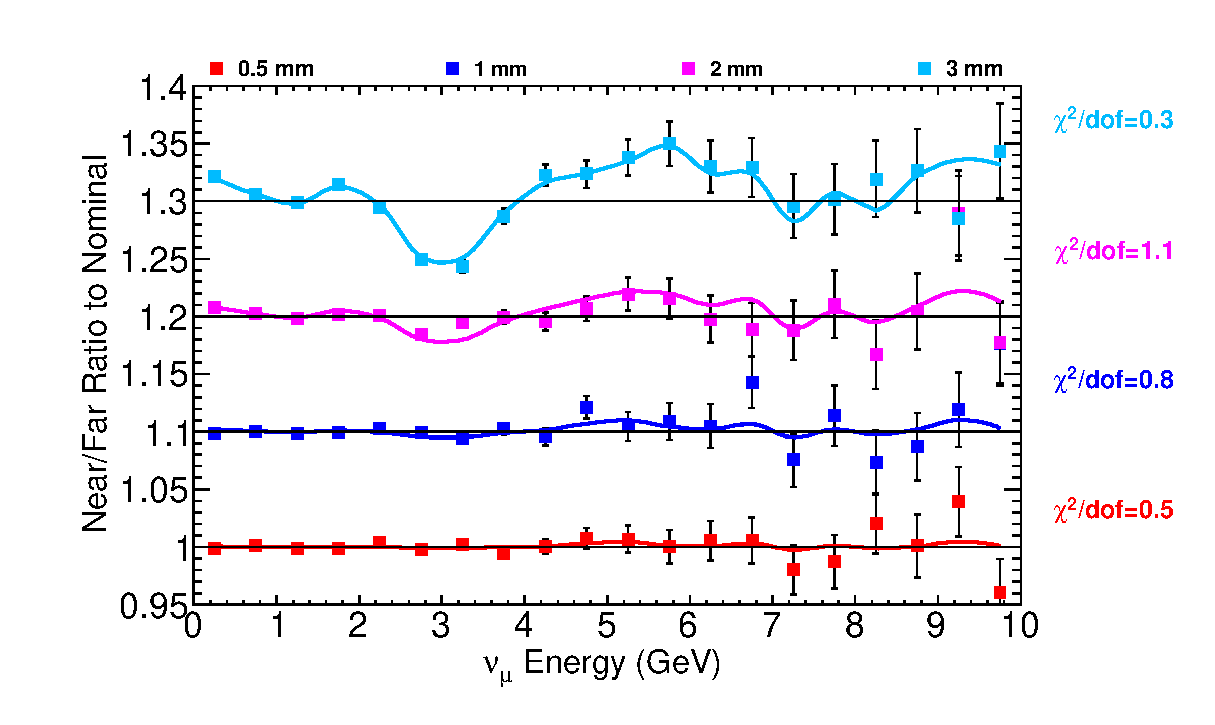
\includegraphics[width=6.0in]{figures/TargetXOffset_nof_summary.eps}}
  \end{center}
\caption{ Near/Far double ratios to nominal for several values of {\bf Target Offset in $x$} (points) and the results of the fits to each energy bin (lines).}
\end{figure}

\begin{figure}[ht]
\label{fig:TargetXOffset_nof_fits}
  \begin{center}
    {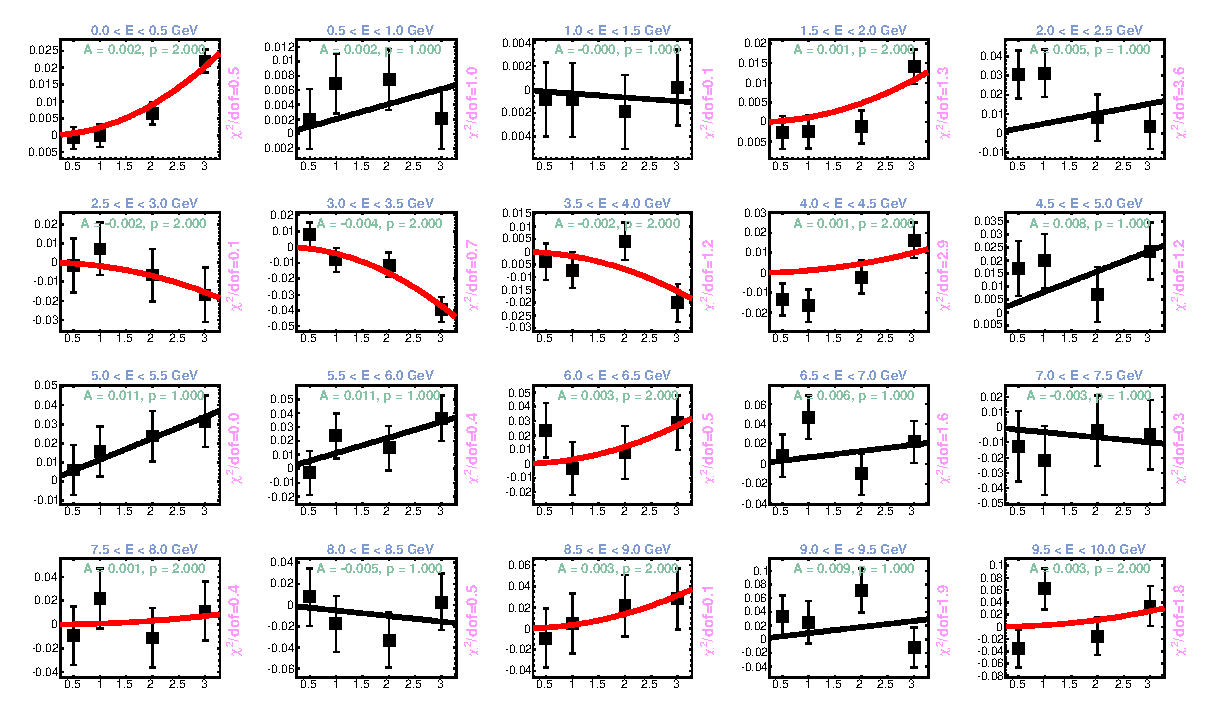
\includegraphics[width=4.0in]{figures/TargetXOffset_nof_fits.eps}}
  \end{center}
\caption{ Fits to the near/far ratios for several values of {\bf Target Offset in $x$}. Black(Red) fit lines indicate that a linear(parabolic) fit provided the best $\chi^2$. }
\end{figure}

\begin{figure}[ht]
\label{fig:TargetXOffset_nof_error}
  \begin{center}
    {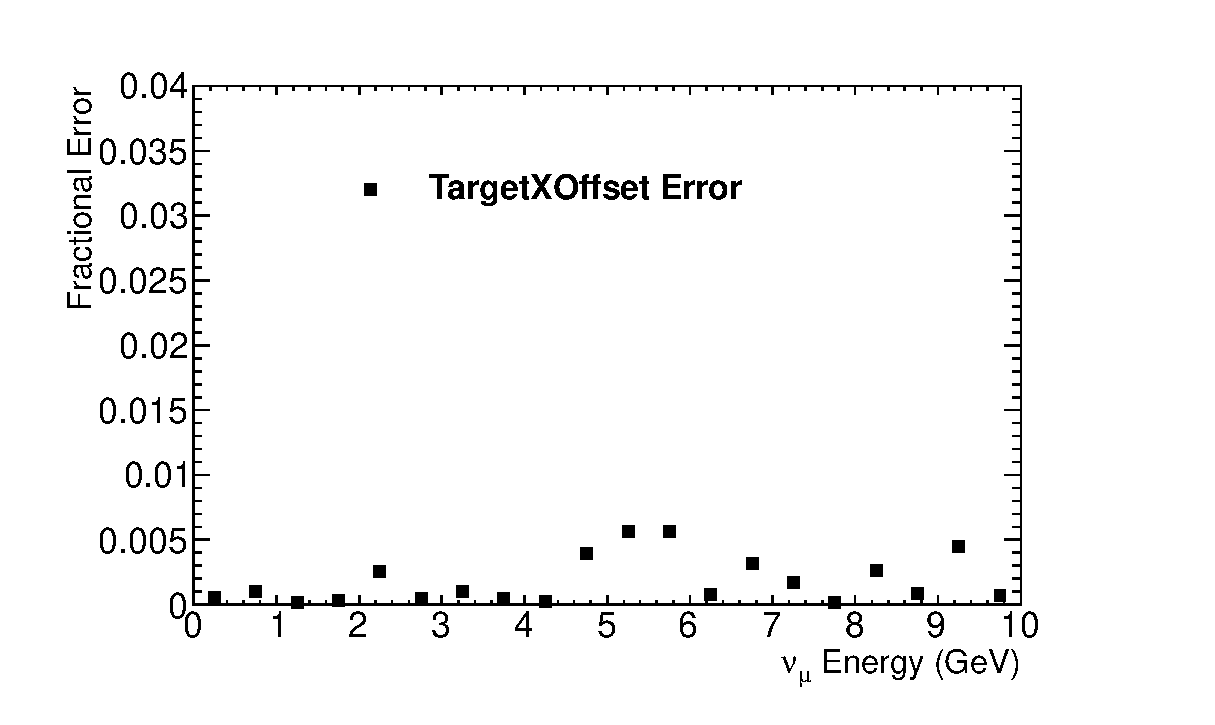
\includegraphics[width=6.0in]{figures/TargetXOffset_nof_error.eps}}
  \end{center}
\caption{ Systematic uncertainty on the near/far flux ratio due to a target offset along the $x$ axis. }
\end{figure}

To study the effect of shielding block alignment, we have simlated the flux with and without shielding blocks present.  The ratio of these is shown in Figure~\ref{fig:shielding_far}. We find find no difference from the nominal configuration beyond statistical fluctuations.  We therefore assume that alignment block shifts of order 1 cm would lead to negligible systematic uncertainties and do not include this source in our total estimat of alignment uncertainties.

\begin{figure}[ht]
\label{fig:shielding_far}
  \begin{center}
    {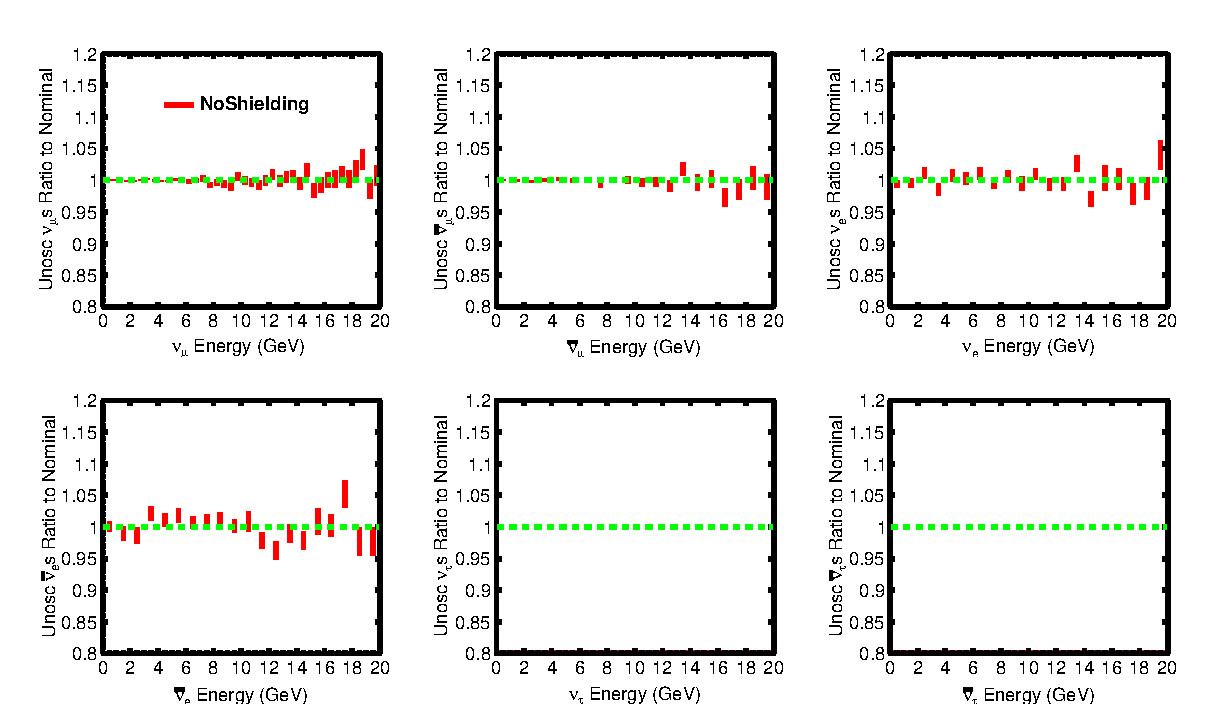
\includegraphics[width=6.0in]{figures/comp_flux_ratios_FHC_unoscillated_Nominal_NoShielding_far.eps}}
  \end{center}
\caption{ The ratio of flux in the far neutrino detector without shielding blocks to the nominal flux produced with shielding blocks included in the geometry simulation. }
\end{figure}

For the baffle scraping uncertainty, we estimate the flux from the baffle by simulating a point-like beam fired directly at the baffle. Specifically, we simulate a beam with a 0.001 mm standard deviation in width and height offset from the origin by 7 mm.  The flux resulting from aiming the beam at several positions on the baffle in shown in figure~\ref{fig:baffle_flux}.  We then estimate baffle uncertainty by taking 0.25% (the baffle scraping tolerance) of the baffle flux.  The resulting systematic uncertainty is shown in Figure~\ref{fig:baffle_error}.

\begin{figure}[ht]
\label{fig:baffle_flux}
  \begin{center}
    {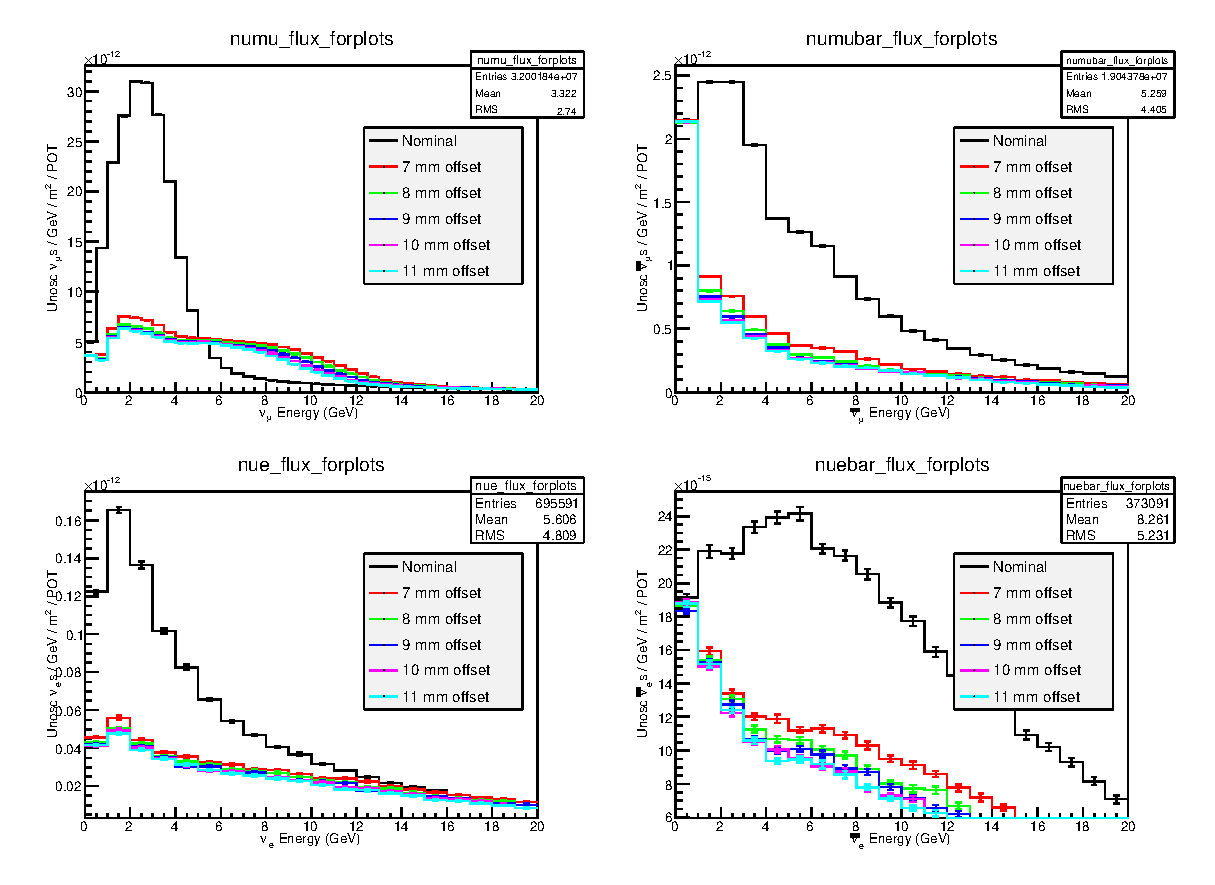
\includegraphics[width=6.0in]{figures/baffle_flux.eps}}
  \end{center}
\caption{ Fluxes at the far detector in the nominal configuration (with the centered on the graphite target) and with the beam directed at various points on the baffle. }
\end{figure}

\begin{figure}[ht]
\label{fig:baffle_error}
  \begin{center}
    {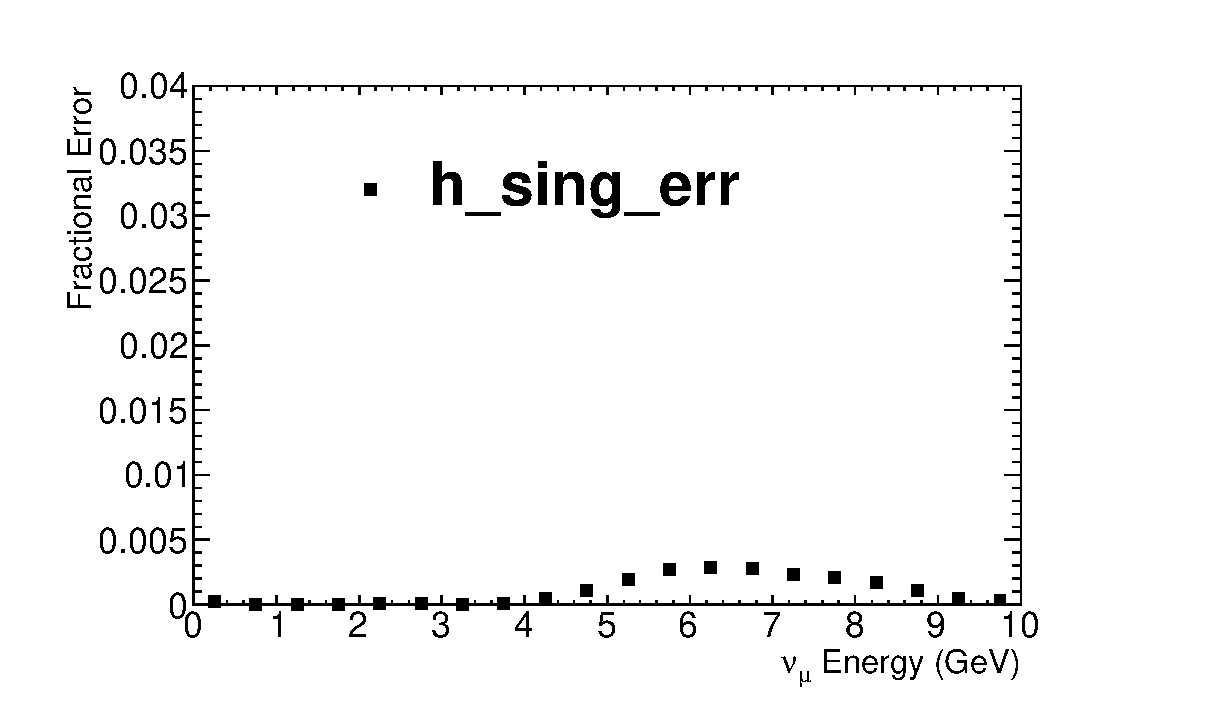
\includegraphics[width=6.0in]{figures/BeamOffsetX7Sigma0pnt001_nof_error.eps}}
  \end{center}
\caption{ Systematic uncertainty on the near/far flux ratio due to baffle scraping. }
\end{figure}


\section{Results}
\label{sec:results}

\begin{sidewaystable}[ht]
\centering
\tiny
\begin{tabular}{|c | c c c c c c c c c c c c c c c c c c c c | }
\hline
Energy( GeV) & 0-0.5 & 0.5-1 & 1-1.5 & 1.5-2 & 2-2.5 & 2.5-3 & 3-3.5 & 3.5-4 & 4-4.5 & 4.5-5 & 5-5.5 & 5.5-6 & 6-6.5 & 6.5-7 & 7-7.5 & 7.5-8 & 8-8.5 & 8.5-9 & 9-9.5 & 9.5-10 \\
\hline
Far Det Offset X & 0.00
 & 0.00
 & 0.01
 & 0.00
 & 0.00
 & 0.00
 & 0.00
 & 0.00
 & 0.00
 & 0.00
 & 0.02
 & 0.00
 & 0.00
 & 0.00
 & 0.00
 & 0.00
 & 0.07
 & 0.04
 & 0.00
 & 0.01
\\
Far Det Offset Y & 0.00
 & 0.00
 & 0.01
 & 0.00
 & 0.00
 & 0.00
 & 0.00
 & 0.03
 & 0.00
 & 0.00
 & 0.04
 & 0.03
 & 0.00
 & 0.00
 & 0.00
 & 0.00
 & 0.04
 & 0.00
 & 0.01
 & 0.00
\\
Near Det Offset X & 0.01
 & 0.00
 & 0.00
 & 0.02
 & 0.01
 & 0.00
 & 0.00
 & 0.01
 & 0.00
 & 0.01
 & 0.01
 & 0.02
 & 0.02
 & 0.24
 & 0.01
 & 0.03
 & 0.00
 & 0.12
 & 0.06
 & 0.03
\\
Near Det Offset Y & 0.01
 & 0.00
 & 0.00
 & 0.02
 & 0.01
 & 0.00
 & 0.00
 & 0.01
 & 0.00
 & 0.01
 & 0.00
 & 0.01
 & 0.01
 & 0.01
 & 0.03
 & 0.07
 & 0.00
 & 0.07
 & 0.10
 & 0.00
\\
Horn Current & 0.04
 & 0.03
 & 0.01
 & 0.02
 & 0.04
 & 0.19
 & 0.64
 & 1.05
 & 0.74
 & 0.40
 & 0.23
 & 0.52
 & 0.46
 & 0.23
 & 0.21
 & 0.31
 & 0.04
 & 0.30
 & 0.11
 & 0.05
\\
Horn 1 X Tilt & 0.02
 & 0.01
 & 0.01
 & 0.00
 & 0.02
 & 0.03
 & 0.01
 & 0.00
 & 0.02
 & 0.23
 & 0.14
 & 0.02
 & 0.10
 & 0.01
 & 0.27
 & 0.37
 & 0.05
 & 0.17
 & 0.60
 & 0.09
\\
Horn 1 Y Tilt & 0.03
 & 0.00
 & 0.01
 & 0.00
 & 0.06
 & 0.00
 & 0.09
 & 0.10
 & 0.07
 & 0.04
 & 0.03
 & 0.59
 & 0.06
 & 0.34
 & 0.05
 & 0.33
 & 0.60
 & 0.54
 & 0.26
 & 0.58
\\
Horn 1 X Offset & 0.01
 & 0.00
 & 0.01
 & 0.01
 & 0.01
 & 0.09
 & 0.03
 & 0.05
 & 0.07
 & 0.74
 & 0.10
 & 0.02
 & 0.19
 & 0.15
 & 0.10
 & 0.37
 & 0.10
 & 0.11
 & 0.16
 & 0.12
\\
Horn 1 Y Offset & 0.02
 & 0.00
 & 0.02
 & 0.00
 & 0.00
 & 0.02
 & 0.11
 & 0.02
 & 0.03
 & 0.12
 & 0.00
 & 0.03
 & 0.42
 & 0.03
 & 0.20
 & 0.05
 & 0.07
 & 0.06
 & 0.26
 & 0.77
\\
Horn 2 X Offset & 0.01
 & 0.00
 & 0.02
 & 0.03
 & 0.02
 & 0.02
 & 0.03
 & 0.05
 & 0.01
 & 0.02
 & 0.03
 & 0.04
 & 0.05
 & 0.06
 & 0.84
 & 0.03
 & 0.23
 & 0.17
 & 0.66
 & 0.13
\\
Horn 2 Y Offset & 0.00
 & 0.00
 & 0.00
 & 0.01
 & 0.01
 & 0.01
 & 0.02
 & 0.02
 & 0.05
 & 0.03
 & 0.22
 & 0.09
 & 0.03
 & 0.08
 & 0.03
 & 0.06
 & 0.04
 & 0.05
 & 0.02
 & 0.07
\\
Horn 2 X Tilt & 0.00
 & 0.00
 & 0.00
 & 0.00
 & 0.04
 & 0.00
 & 0.04
 & 0.03
 & 0.10
 & 0.02
 & 0.05
 & 0.01
 & 0.05
 & 0.28
 & 0.06
 & 0.09
 & 0.10
 & 0.14
 & 0.33
 & 0.20
\\
Horn 2 Y Tilt & 0.00
 & 0.01
 & 0.00
 & 0.00
 & 0.02
 & 0.01
 & 0.02
 & 0.00
 & 0.02
 & 0.33
 & 0.05
 & 0.04
 & 0.14
 & 0.04
 & 0.18
 & 0.29
 & 0.31
 & 0.88
 & 0.71
 & 1.27
\\
Target X Offset & 0.04
 & 0.01
 & 0.03
 & 0.03
 & 0.01
 & 0.10
 & 0.10
 & 0.02
 & 0.03
 & 0.31
 & 0.45
 & 0.10
 & 0.05
 & 0.30
 & 0.22
 & 0.09
 & 0.10
 & 0.05
 & 0.46
 & 0.07
\\
Target Y Offset & 0.00
 & 0.01
 & 0.02
 & 0.01
 & 0.01
 & 0.02
 & 0.00
 & 0.01
 & 0.27
 & 0.01
 & 0.17
 & 0.04
 & 0.08
 & 0.19
 & 0.17
 & 0.03
 & 0.38
 & 0.58
 & 0.56
 & 0.83
\\
Target X Tilt & 0.03
 & 0.01
 & 0.01
 & 0.07
 & 0.01
 & 0.08
 & 0.06
 & 0.00
 & 0.02
 & 0.03
 & 0.40
 & 0.04
 & 0.04
 & 0.08
 & 0.04
 & 0.47
 & 0.05
 & 0.10
 & 0.02
 & 0.28
\\
Target Y Tilt & 0.01
 & 0.01
 & 0.01
 & 0.00
 & 0.00
 & 0.05
 & 0.03
 & 0.01
 & 0.01
 & 0.00
 & 0.09
 & 0.18
 & 0.01
 & 0.34
 & 0.03
 & 0.37
 & 0.54
 & 0.33
 & 0.05
 & 0.57
\\
Beam Width X & 0.12
 & 0.04
 & 0.00
 & 0.02
 & 0.00
 & 0.00
 & 0.05
 & 0.16
 & 0.25
 & 0.25
 & 0.18
 & 0.01
 & 0.02
 & 0.39
 & 0.58
 & 0.02
 & 0.07
 & 0.35
 & 0.08
 & 0.07
\\
Beam Width Y & 0.00
 & 0.00
 & 0.01
 & 0.02
 & 0.03
 & 0.00
 & 0.05
 & 0.03
 & 0.07
 & 0.03
 & 0.11
 & 0.10
 & 0.20
 & 0.06
 & 0.13
 & 0.08
 & 0.11
 & 0.21
 & 0.05
 & 0.07
\\
Decay Pipe Radius & 0.22
 & 0.81
 & 1.10
 & 0.15
 & 0.84
 & 0.90
 & 0.64
 & 0.40
 & 0.15
 & 0.02
 & 0.01
 & 0.02
 & 0.23
 & 0.05
 & 0.04
 & 0.05
 & 0.05
 & 0.46
 & 0.08
 & 0.44
\\
Water Layer Thickness & 0.10
 & 0.02
 & 0.01
 & 0.09
 & 0.03
 & 0.18
 & 0.17
 & 0.05
 & 0.06
 & 0.18
 & 0.89
 & 0.13
 & 0.20
 & 0.26
 & 0.73
 & 0.41
 & 0.60
 & 0.13
 & 0.25
 & 1.54
\\
Baffle Scraping & 0.02
 & 0.00
 & 0.00
 & 0.00
 & 0.01
 & 0.01
 & 0.00
 & 0.01
 & 0.05
 & 0.11
 & 0.19
 & 0.27
 & 0.29
 & 0.28
 & 0.23
 & 0.21
 & 0.17
 & 0.11
 & 0.05
 & 0.03
\\
Decay Pipe Shift X & 0.01
 & 0.00
 & 0.00
 & 0.00
 & 0.00
 & 0.00
 & 0.00
 & 0.00
 & 0.00
 & 0.04
 & 0.00
 & 0.01
 & 0.00
 & 0.03
 & 0.03
 & 0.00
 & 0.00
 & 0.01
 & 0.07
 & 0.01
\\
IC Skin Depth & 0.03
 & 0.03
 & 0.05
 & 0.08
 & 0.09
 & 0.09
 & 0.11
 & 0.32
 & 0.56
 & 0.19
 & 0.66
 & 1.27
 & 0.13
 & 0.34
 & 0.54
 & 1.85
 & 0.59
 & 1.22
 & 2.38
 & 0.60
\\
BeamTilt X & 0.00
 & 0.00
 & 0.00
 & 0.00
 & 0.00
 & 0.00
 & 0.00
 & 0.00
 & 0.00
 & 0.00
 & 0.01
 & 0.01
 & 0.01
 & 0.01
 & 0.01
 & 0.01
 & 0.01
 & 0.01
 & 0.13
 & 0.06
\\
BeamTilt Y & 0.00
 & 0.00
 & 0.00
 & 0.00
 & 0.00
 & 0.01
 & 0.00
 & 0.00
 & 0.00
 & 0.00
 & 0.01
 & 0.01
 & 0.01
 & 0.01
 & 0.01
 & 0.01
 & 0.00
 & 0.03
 & 0.13
 & 0.00
\\
Beam Offset X & 0.17
 & 0.06
 & 0.02
 & 0.06
 & 0.04
 & 0.02
 & 0.04
 & 0.11
 & 0.20
 & 0.22
 & 0.18
 & 0.06
 & 0.15
 & 0.29
 & 0.49
 & 0.06
 & 0.08
 & 0.09
 & 0.32
 & 0.22
\\
Beam Offset Y & 0.01
 & 0.01
 & 0.00
 & 0.01
 & 0.00
 & 0.11
 & 0.03
 & 0.02
 & 0.03
 & 0.08
 & 0.08
 & 0.06
 & 0.26
 & 0.04
 & 0.07
 & 0.11
 & 0.01
 & 0.03
 & 0.40
 & 0.05
\\

\hline
\end{tabular}
\label{tab:errorsummary}
\caption{Systematic errors on the near/far ratio (in percent) in each energy bin for each source of alignment uncertainty.}
\end{sidewaystable}


\begin{figure}[ht]
  \begin{center}
    {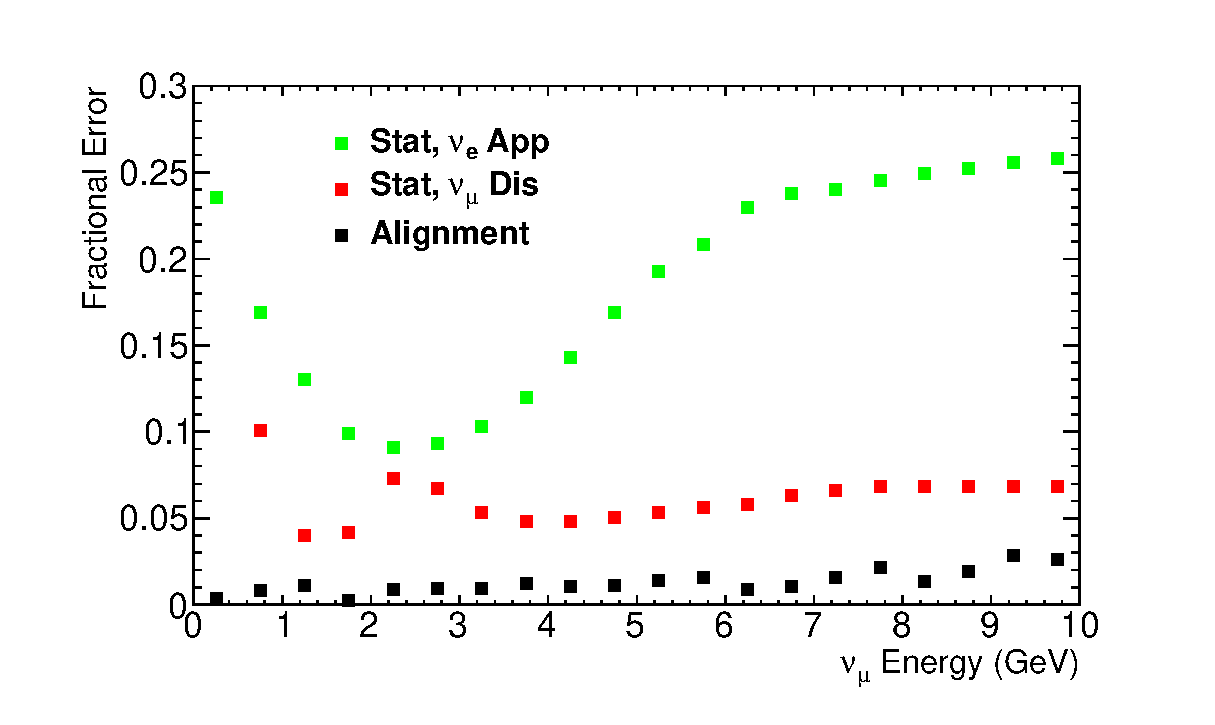
\includegraphics[width=6.0in]{figures/tot_error_nof.eps}}
  \end{center}
\caption{ Total fractional alignment systematic uncertainty as a function of energy on the near/far flux ratio. }
\end{figure}

\begin{figure}[ht]
  \begin{center}
    {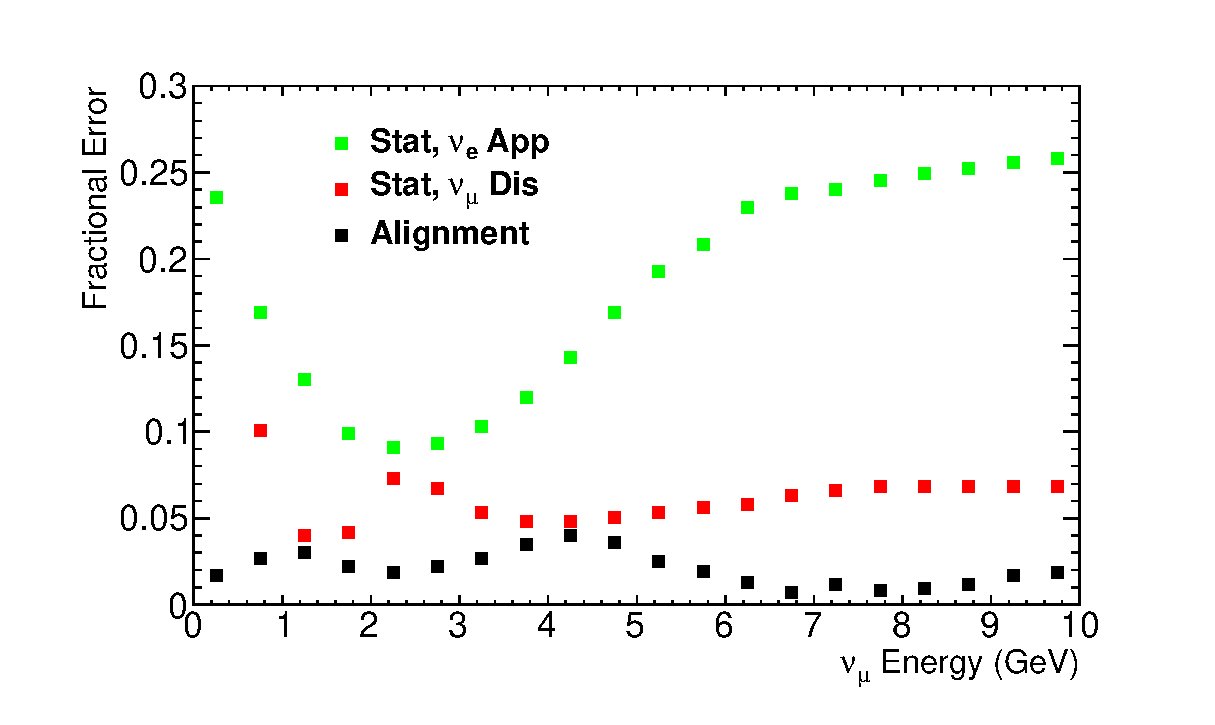
\includegraphics[width=6.0in]{figures/tot_error_near.eps}}
  \end{center}
\caption{ Total fractional alignment systematic uncertainty as a function of energy on the flux at the near detector. }
\end{figure}

\begin{figure}[ht]
  \begin{center}
    {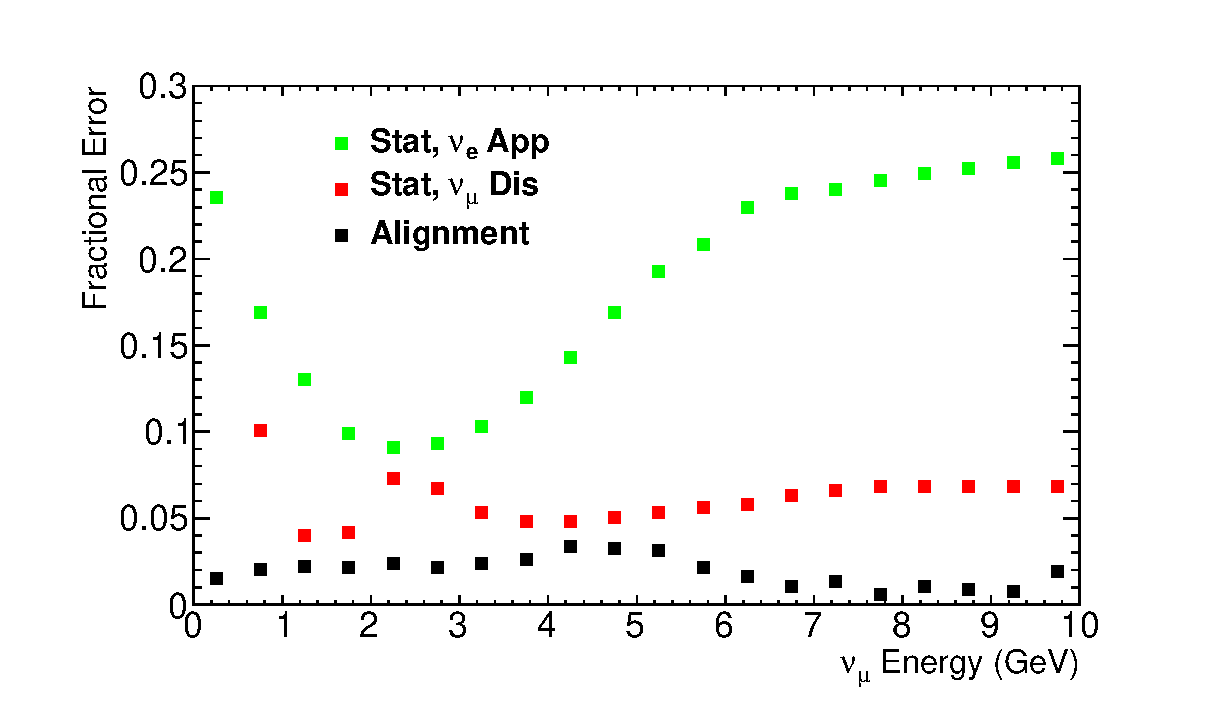
\includegraphics[width=6.0in]{figures/tot_error_far.eps}}
  \end{center}
\caption{ Total fractional alignment systematic uncertainty as a function of energy on the flux at the far detector. }
\end{figure}

\begin{figure}[ht]
  \begin{center}
    {
\includegraphics[width=6.0in]{figures/error_summary_nof.eps}}
  \end{center}
\caption{ Summary of alignment systematic uncertainties on the near/far flux ratio.}
\end{figure}

\begin{figure}[ht]
  \begin{center}
    {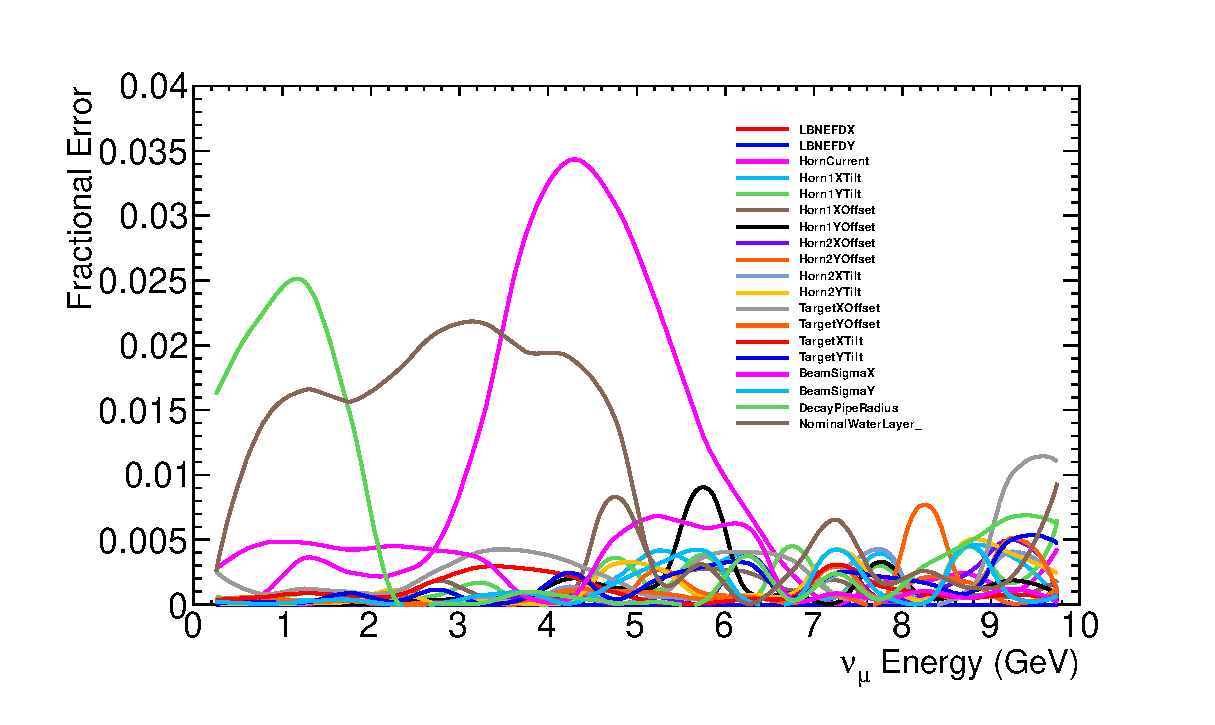
\includegraphics[width=6.0in]{figures/error_summary_near.eps}}
  \end{center}
\caption{ Summary of alignment systematic uncertainties on the flux at the near detector.}
\end{figure}

\begin{figure}[ht]
  \begin{center}
    {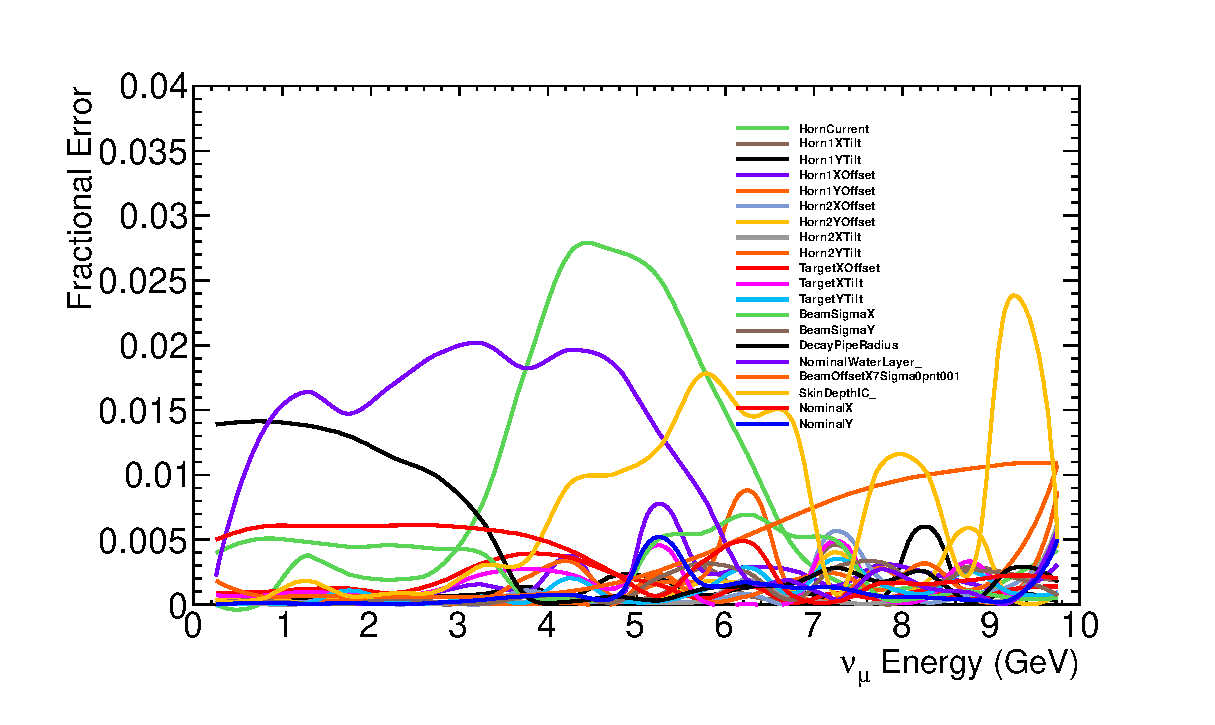
\includegraphics[width=6.0in]{figures/error_summary_far.eps}}
  \end{center}
\caption{ Summary of alignment systematic uncertainties on the flux at the far detector.}
\end{figure}


\section{Conclusion}

\appendix
\section{Near/Far Flux Ratios and Fits}
\label{app:nof_plots}

\subsection{Target Position}

\begin{figure}[ht]
  \begin{center}
    {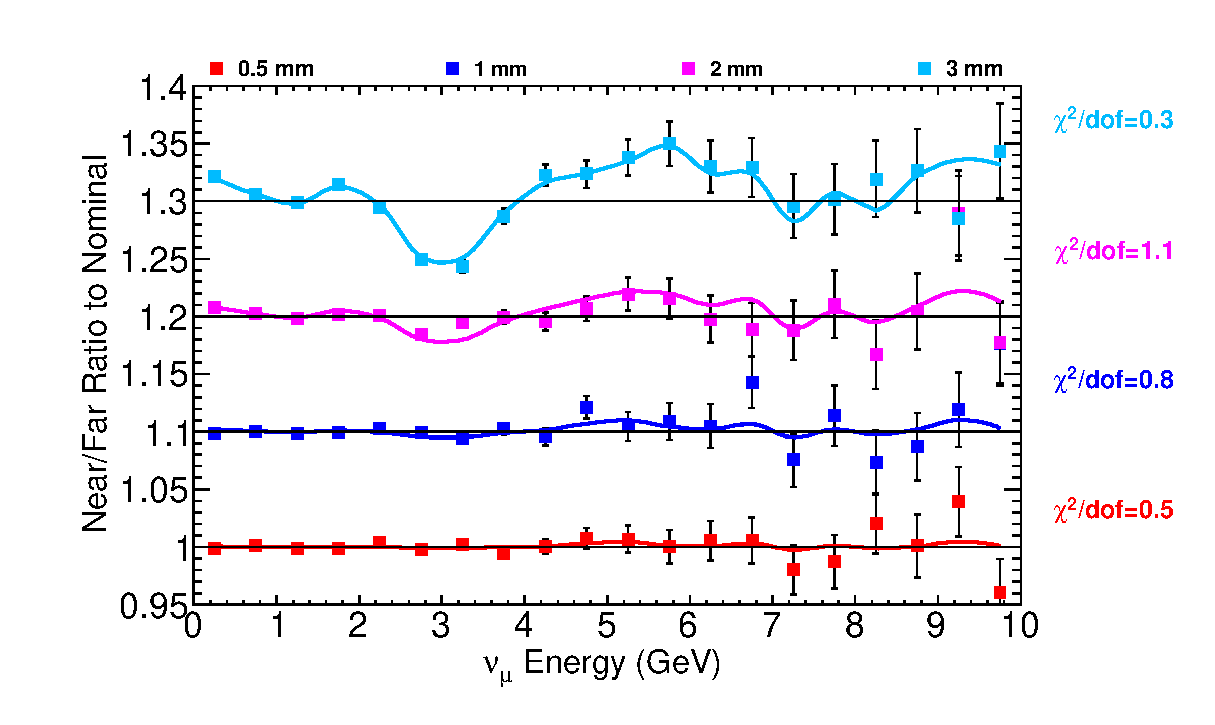
\includegraphics[width=4.0in]{figures/TargetXOffset_nof_summary.eps}}
  \end{center}
\caption{ Near/Far double ratios to nominal for several values of {\bf Target Offset in $x$} (points) and the results of the fits to each energy bin (lines).}
\end{figure}

\begin{figure}[hb]
  \begin{center}
    {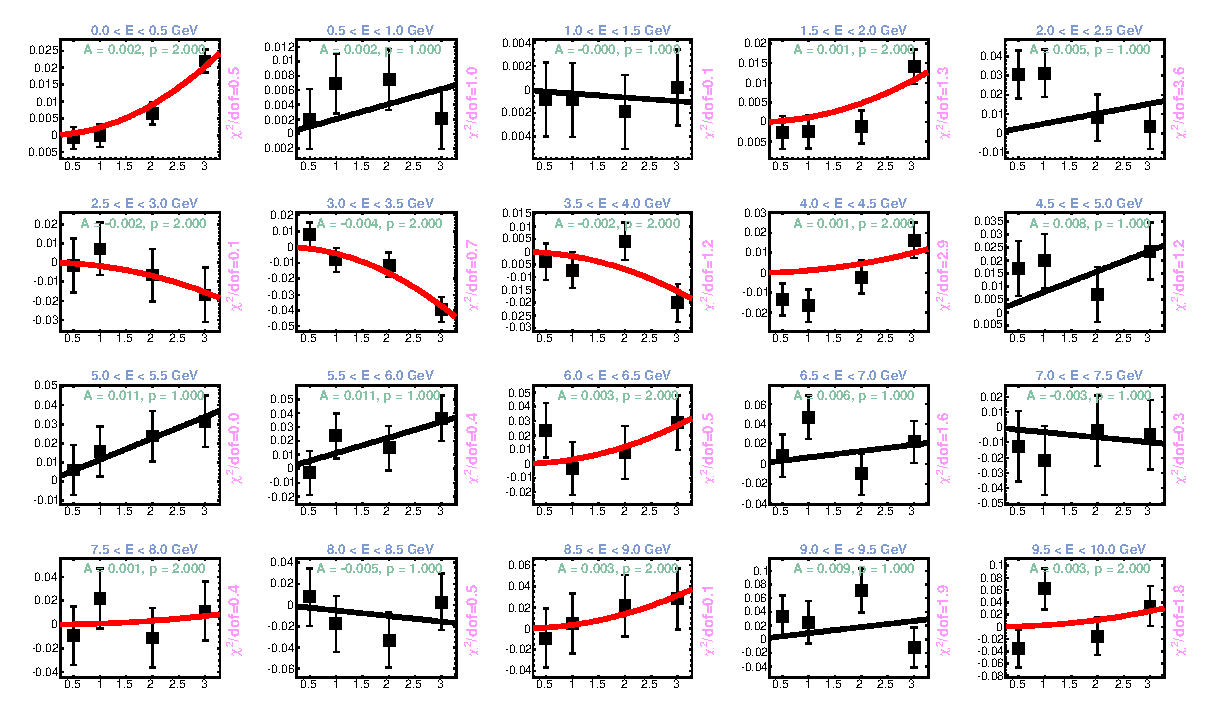
\includegraphics[width=4.0in]{figures/TargetXOffset_nof_fits.eps}}
  \end{center}
\caption{ Fits to the near/far ratios for several values of {\bf Target Offset in $x$}. Black(Red) fit lines indicate that a linear(parabolic) fit provided the best $\chi^2$. }
\end{figure}

\begin{figure}[ht]
  \begin{center}
    {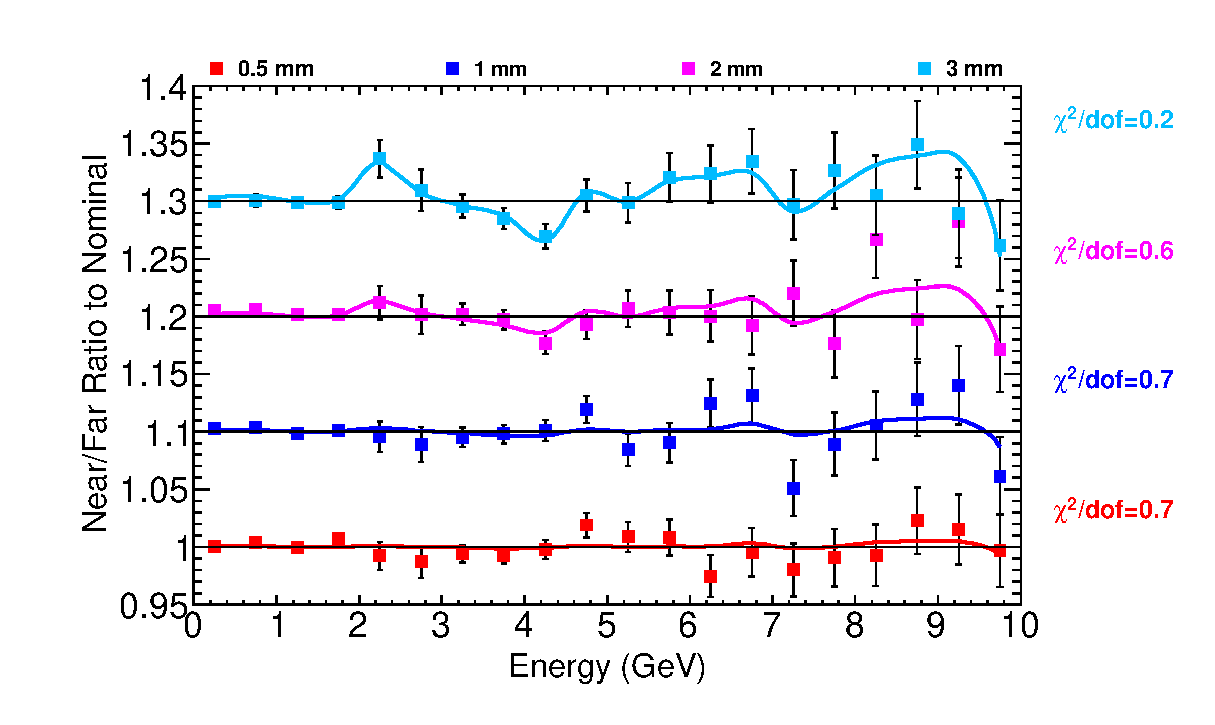
\includegraphics[width=4.0in]{figures/TargetYOffset_nof_summary.eps}}
  \end{center}
\caption{ Near/Far double ratios to nominal for several values of {\bf Target Offset in $y$} (points) and the results of the fits to each energy bin (lines).}
\end{figure}

\begin{figure}[hb]
  \begin{center}
    {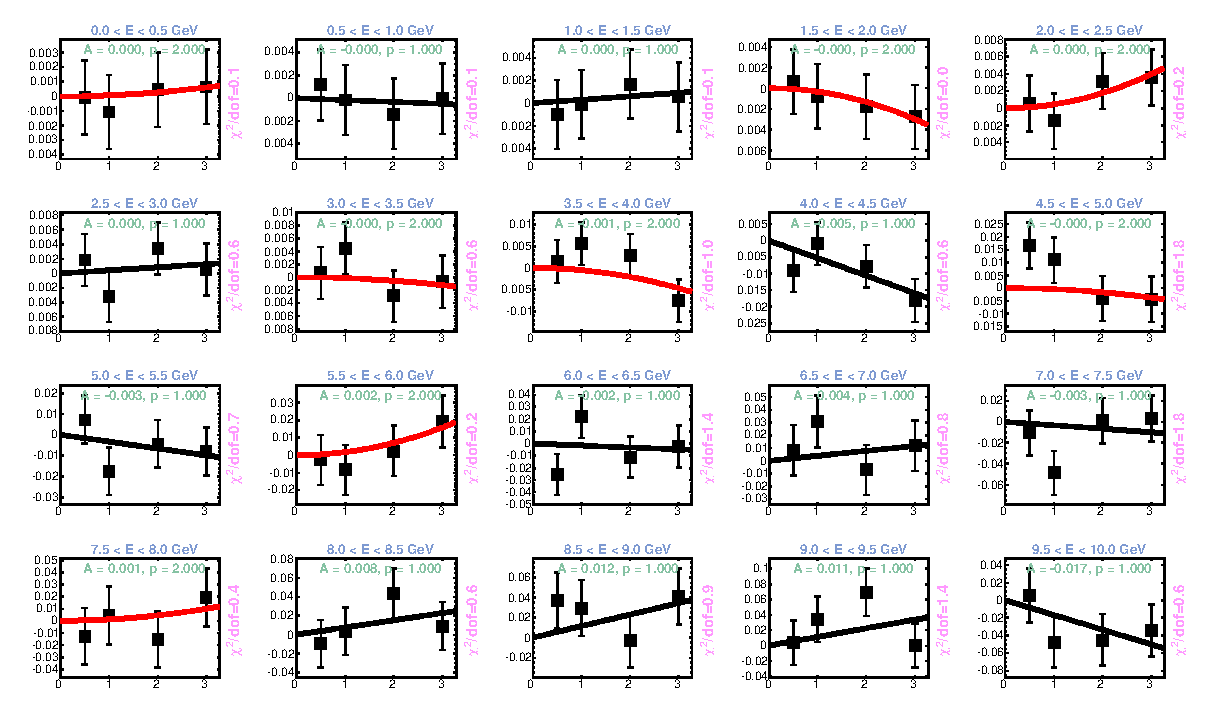
\includegraphics[width=4.0in]{figures/TargetYOffset_nof_fits.eps}}
  \end{center}
\caption{ Fits to the near/far ratios for several values of {\bf Target Offset in $y$}. Black(Red) fit lines indicate that a linear(parabolic) fit provided the best $\chi^2$. }
\end{figure}

\begin{figure}[ht]
  \begin{center}
    {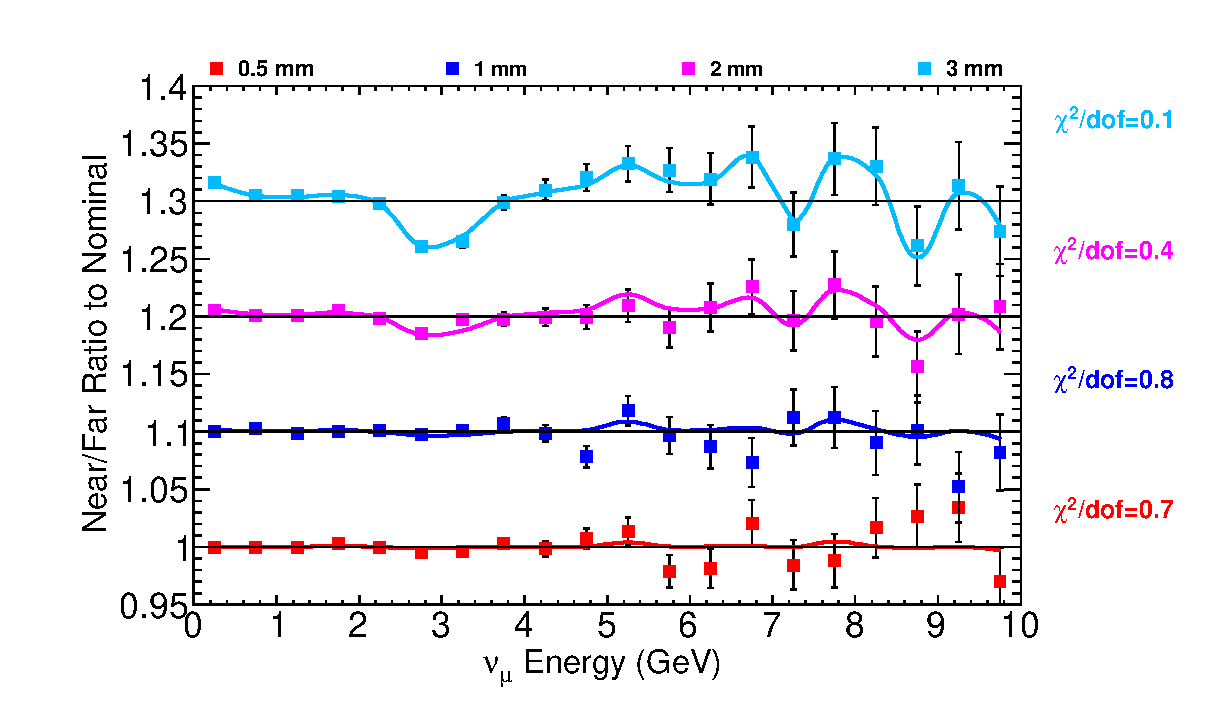
\includegraphics[width=4.0in]{figures/TargetXTilt_nof_summary.eps}}
  \end{center}
\caption{ Near/Far double ratios to nominal for several values of {\bf Target Tilt in $x$} (points) and the results of the fits to each energy bin (lines).}
\end{figure}

\begin{figure}[hb]
  \begin{center}
    {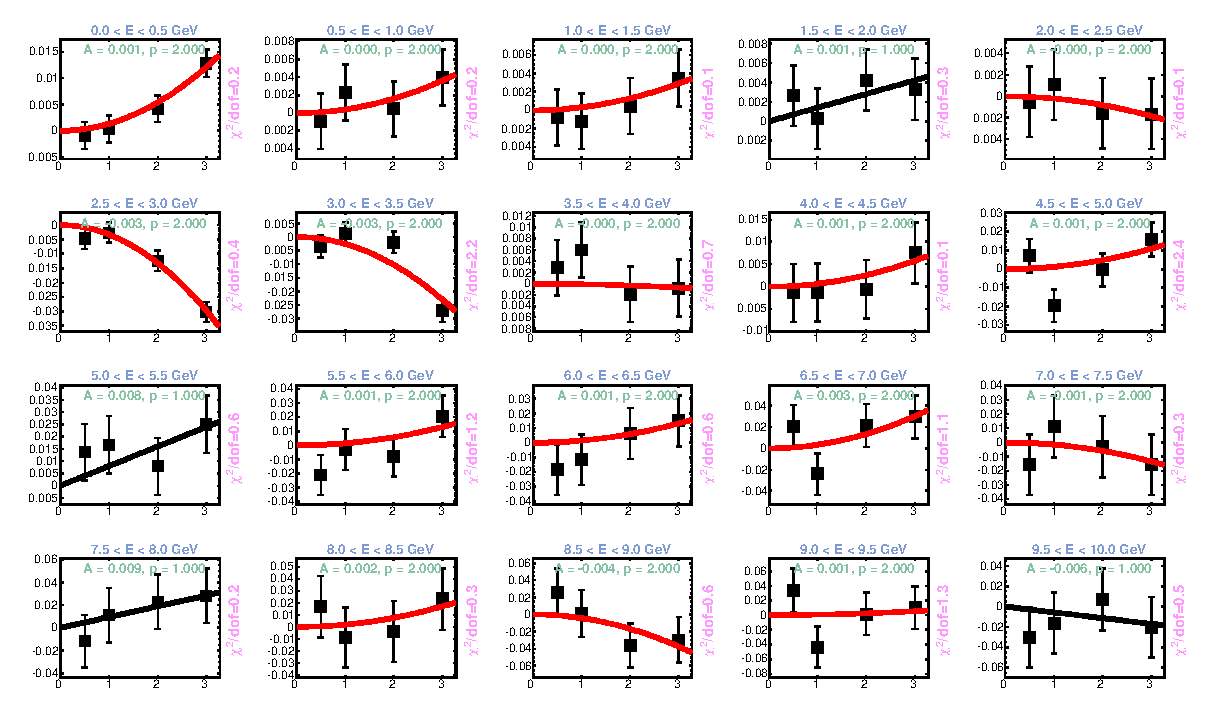
\includegraphics[width=4.0in]{figures/TargetXTilt_nof_fits.eps}}
  \end{center}
\caption{ Fits to the near/far ratios for several values of {\bf Target Tilt in $x$}. Black(Red) fit lines indicate that a linear(parabolic) fit provided the best $\chi^2$. }
\end{figure}

\clearpage
\subsection{Horn 1 Position}

\begin{figure}[ht]
  \begin{center}
    {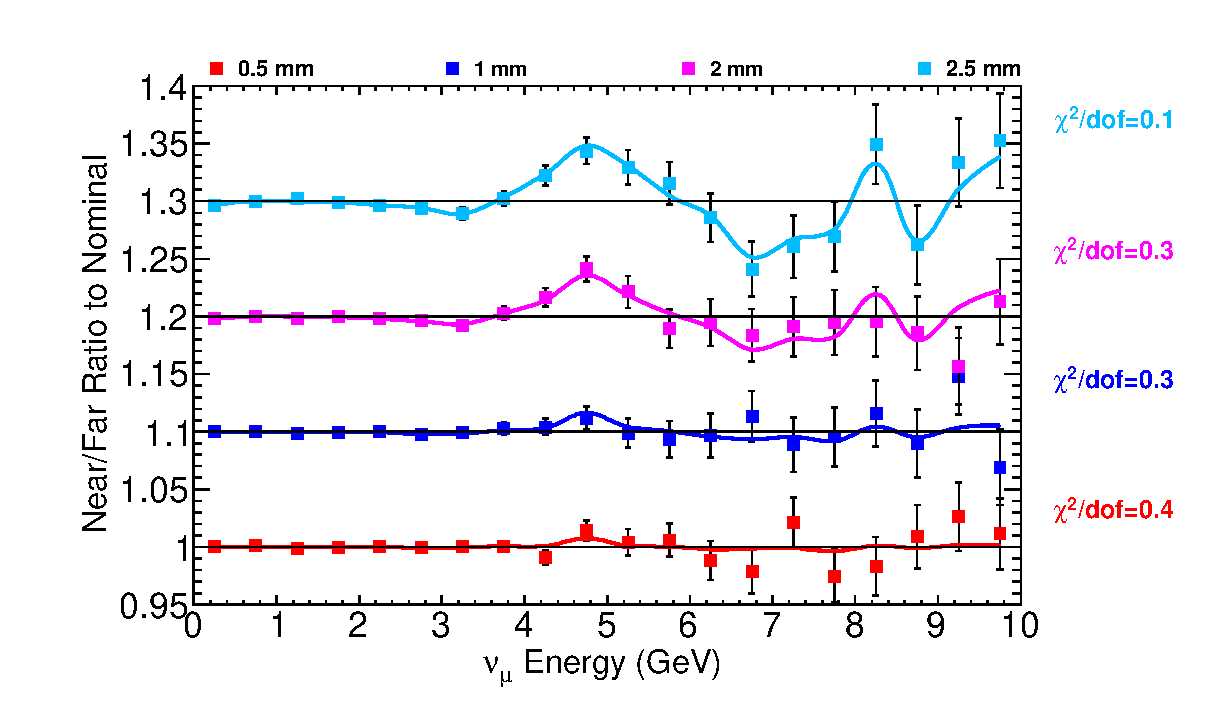
\includegraphics[width=4.0in]{figures/Horn1XOffset_nof_summary.eps}}
  \end{center}
\caption{ Near/Far double ratios to nominal for several values of {\bf Horn 1 Offset in $x$} (points) and the results of the fits to each energy bin (lines).}
\end{figure}

\begin{figure}[hb]
  \begin{center}
    {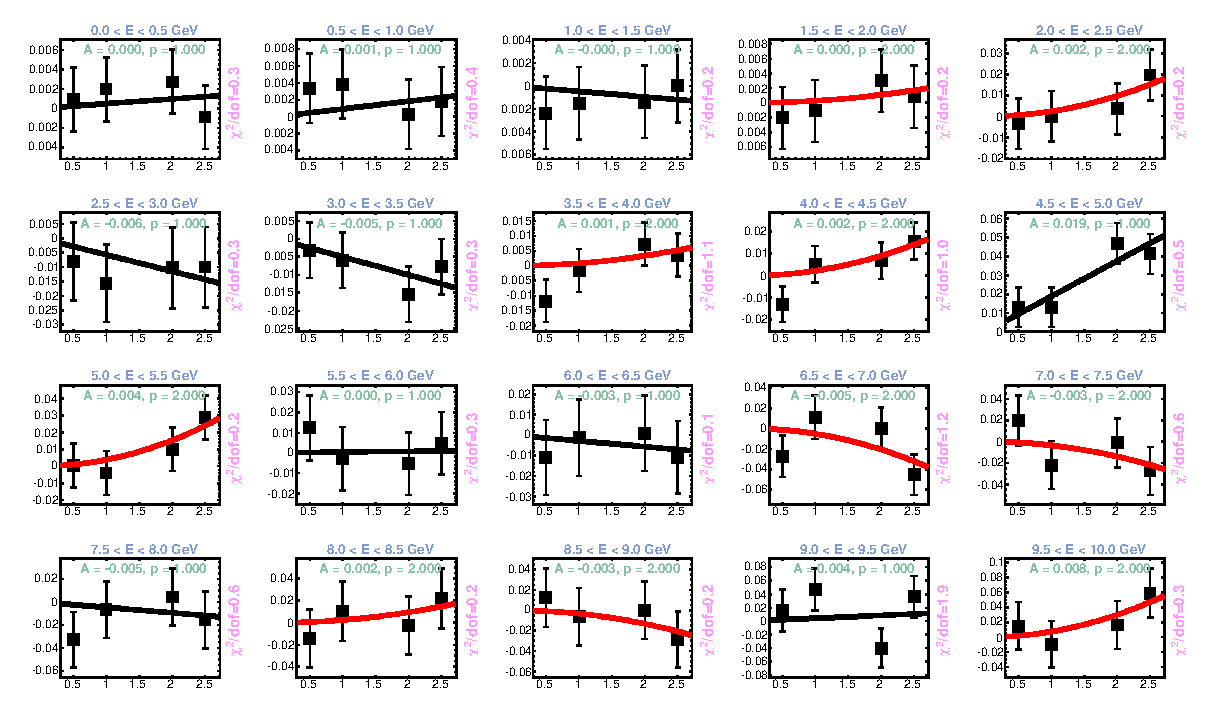
\includegraphics[width=4.0in]{figures/Horn1XOffset_nof_fits.eps}}
  \end{center}
\caption{ Fits to the near/far ratios for several values of {\bf Horn 1 Offset in $x$}. Black(Red) fit lines indicate that a linear(parabolic) fit provided the best $\chi^2$. }
\end{figure}

\begin{figure}[ht]
  \begin{center}
    {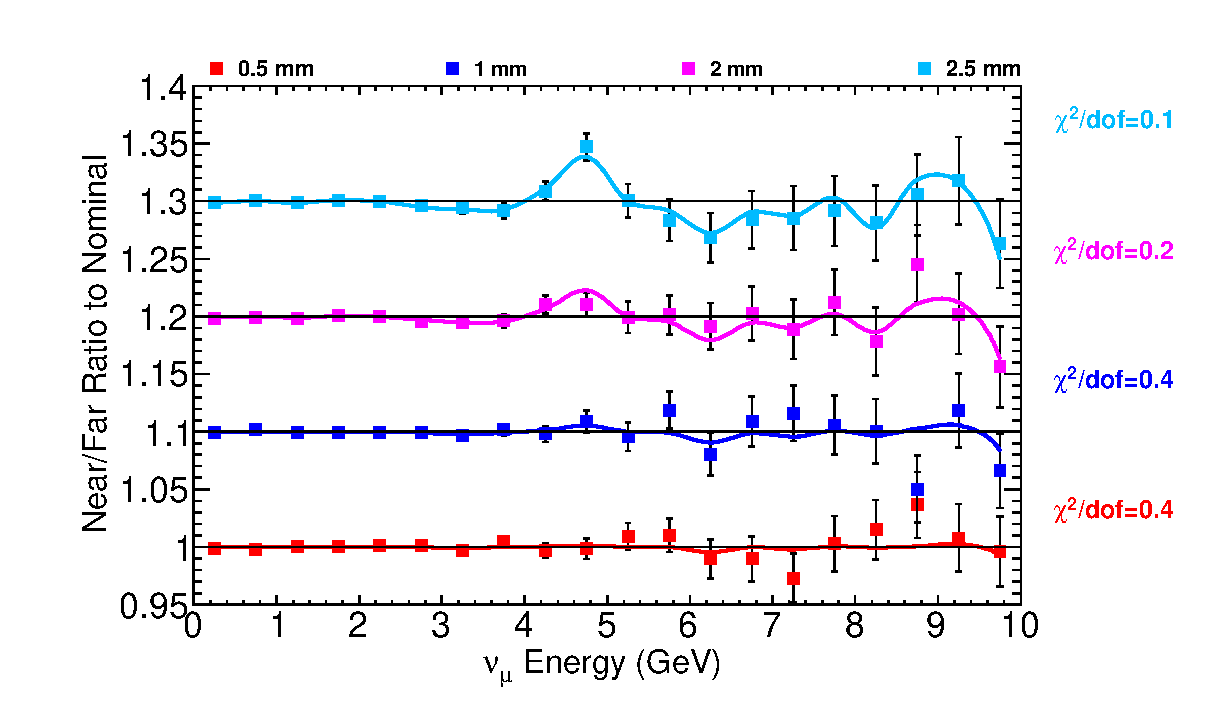
\includegraphics[width=4.0in]{figures/Horn1YOffset_nof_summary.eps}}
  \end{center}
\caption{ Near/Far double ratios to nominal for several values of {\bf Horn 1 Offset in $y$} (points) and the results of the fits to each energy bin (lines).}
\end{figure}

\begin{figure}[hb]
  \begin{center}
    {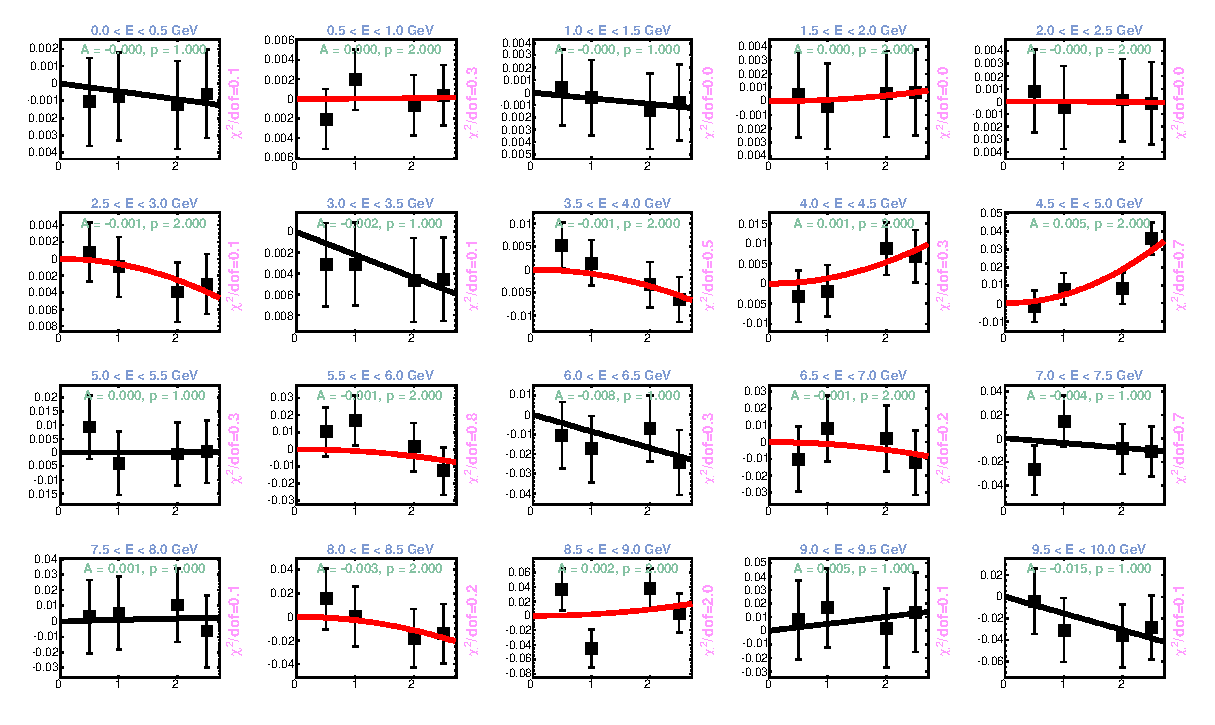
\includegraphics[width=4.0in]{figures/Horn1YOffset_nof_fits.eps}}
  \end{center}
\caption{ Fits to the near/far ratios for several values of {\bf Horn 1 Offset in $y$}. Black(Red) fit lines indicate that a linear(parabolic) fit provided the best $\chi^2$. }
\end{figure}

\begin{figure}[ht]
  \begin{center}
    {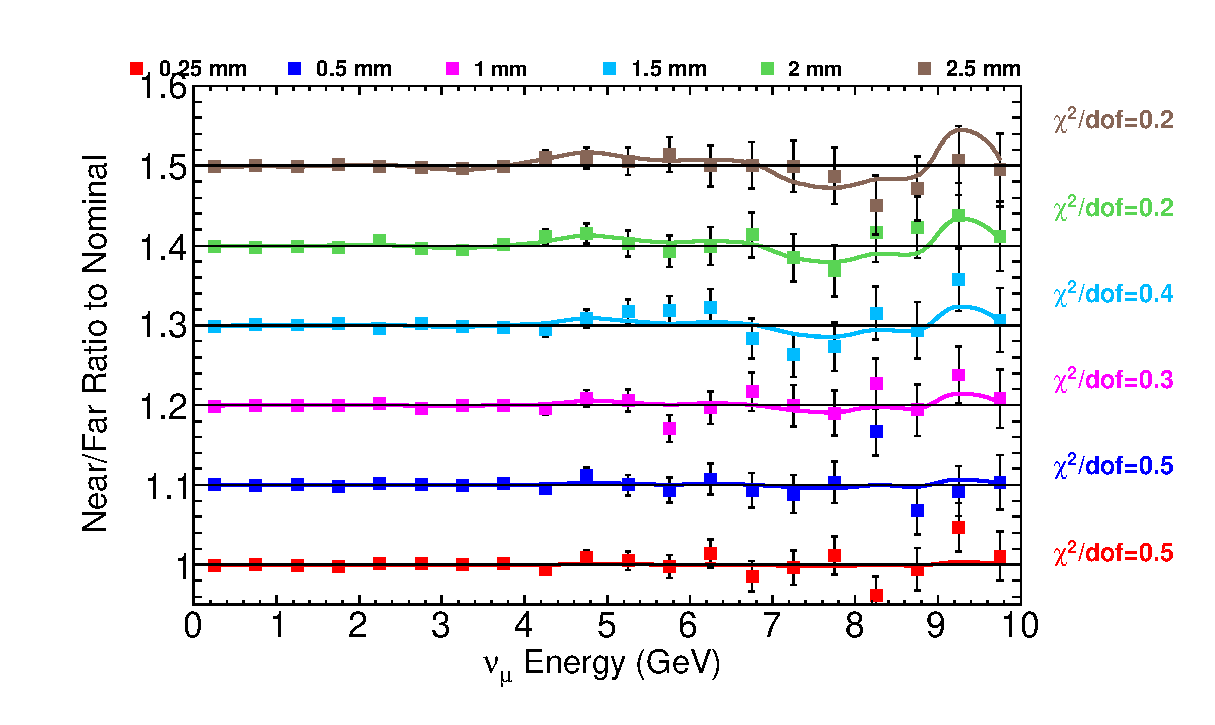
\includegraphics[width=4.0in]{figures/Horn1XTilt_nof_summary.eps}}
  \end{center}
\caption{ Near/Far double ratios to nominal for several values of {\bf Horn 1 Tilt in $x$} (points) and the results of the fits to each energy bin (lines).}
\end{figure}

\begin{figure}[hb]
  \begin{center}
    {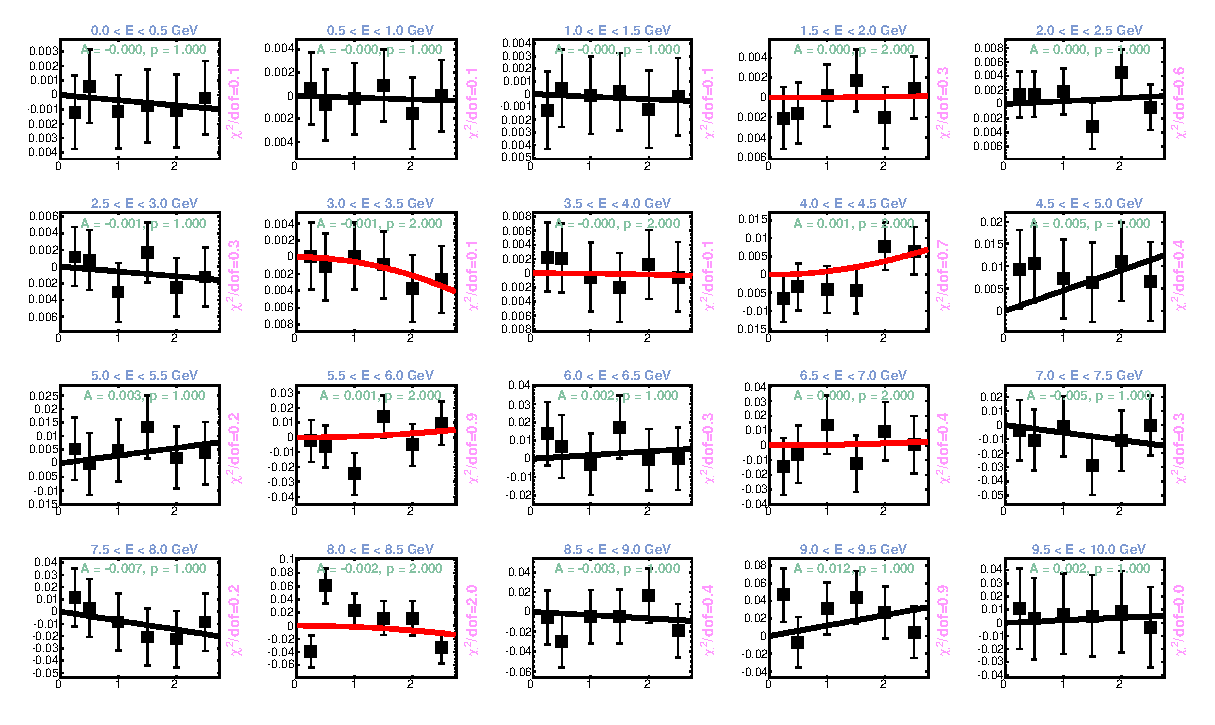
\includegraphics[width=4.0in]{figures/Horn1XTilt_nof_fits.eps}}
  \end{center}
\caption{ Fits to the near/far ratios for several values of {\bf Horn 1 Tilt in $x$}. Black(Red) fit lines indicate that a linear(parabolic) fit provided the best $\chi^2$. }
\end{figure}

\begin{figure}[ht]
  \begin{center}
    {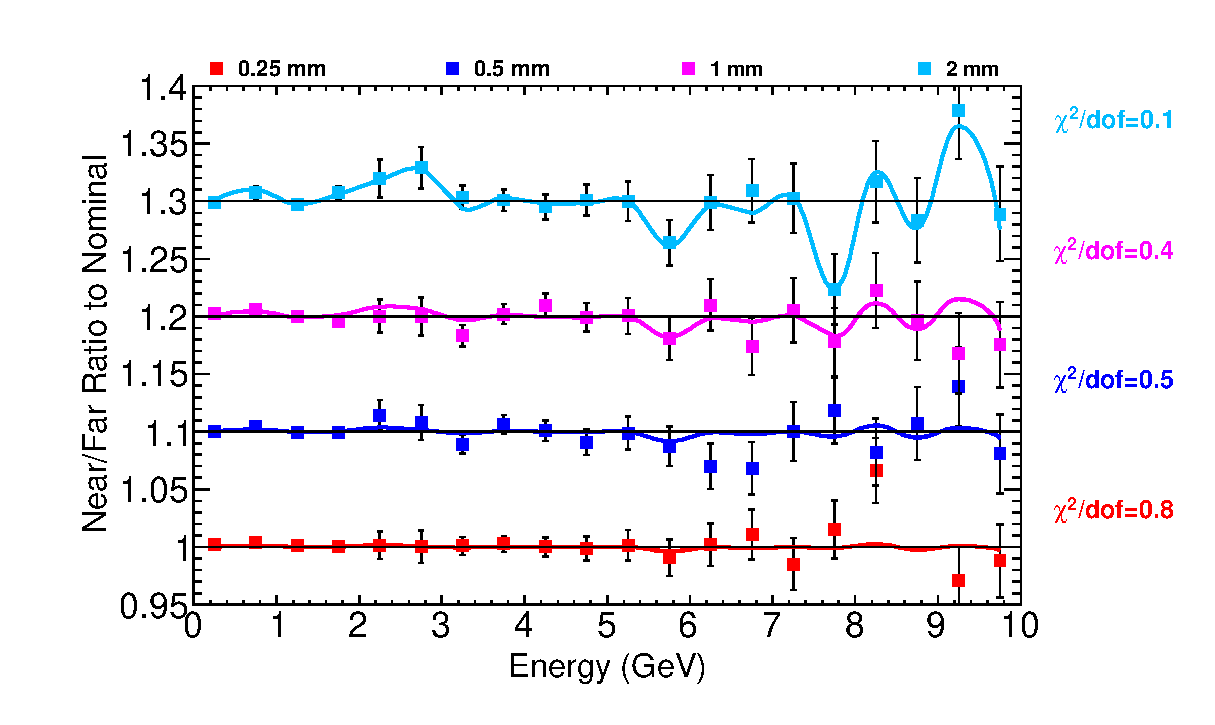
\includegraphics[width=4.0in]{figures/Horn1YTilt_nof_summary.eps}}
  \end{center}
\caption{ Near/Far double ratios to nominal for several values of {\bf Horn 1 Tilt in $y$} (points) and the results of the fits to each energy bin (lines).}
\end{figure}


\begin{figure}[hb]
  \begin{center}
    {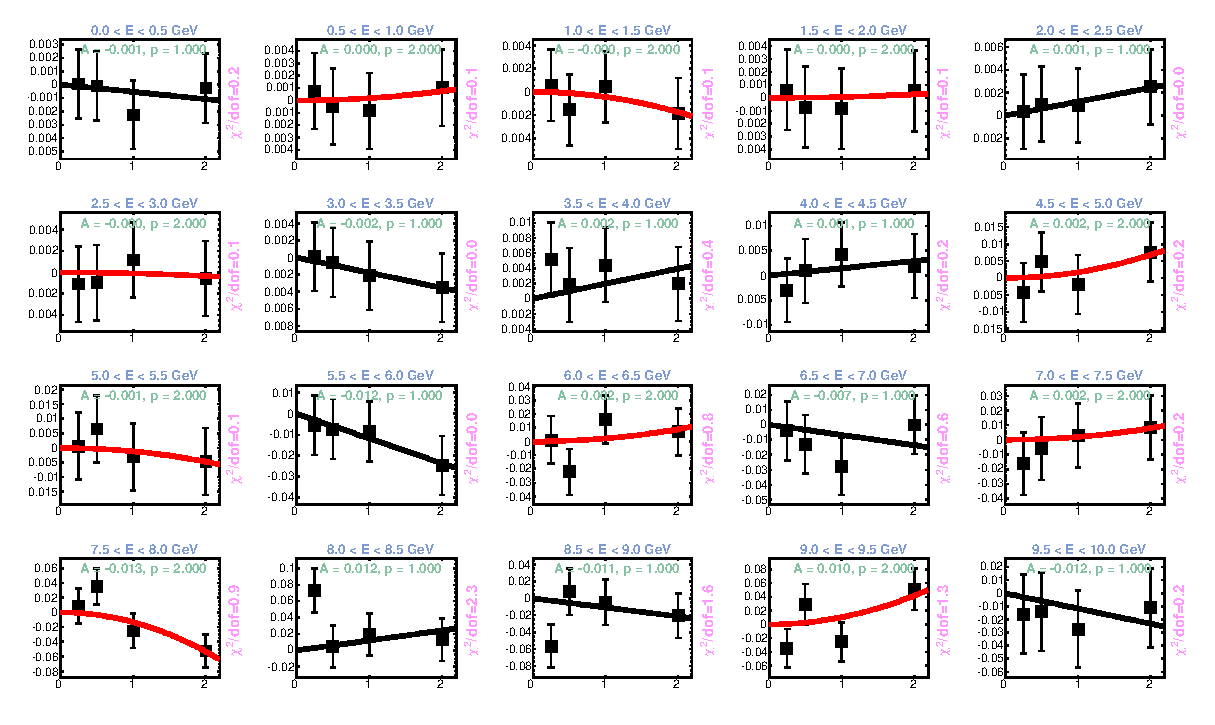
\includegraphics[width=4.0in]{figures/Horn1YTilt_nof_fits.eps}}
  \end{center}
\caption{ Fits to the near/far ratios for several values of {\bf Horn 1 Tilt in $y$}. Black(Red) fit lines indicate that a linear(parabolic) fit provided the best $\chi^2$. }
\end{figure}

\clearpage
\subsection{Horn 2 Position}

\begin{figure}[ht]
  \begin{center}
    {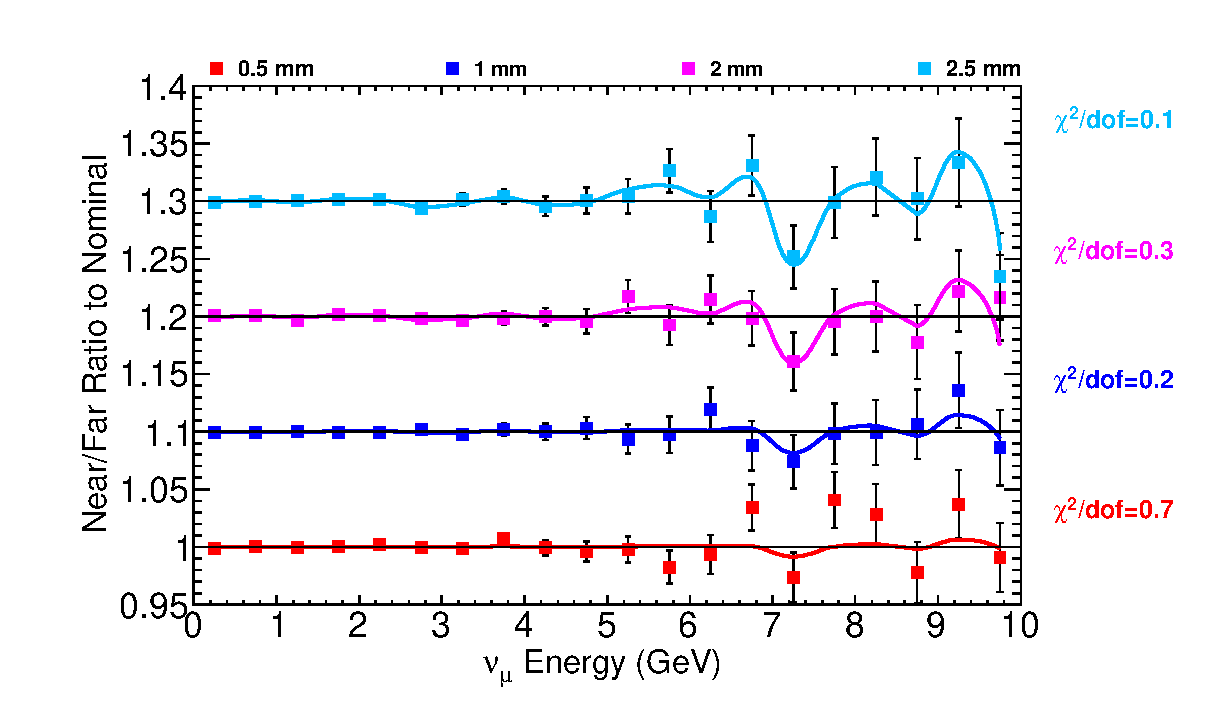
\includegraphics[width=4.0in]{figures/Horn2XOffset_nof_summary.eps}}
  \end{center}
\caption{ Near/Far double ratios to nominal for several values of {\bf Horn 2 Offset in $x$} (points) and the results of the fits to each energy bin (lines).}
\end{figure}

\begin{figure}[hb]
  \begin{center}
    {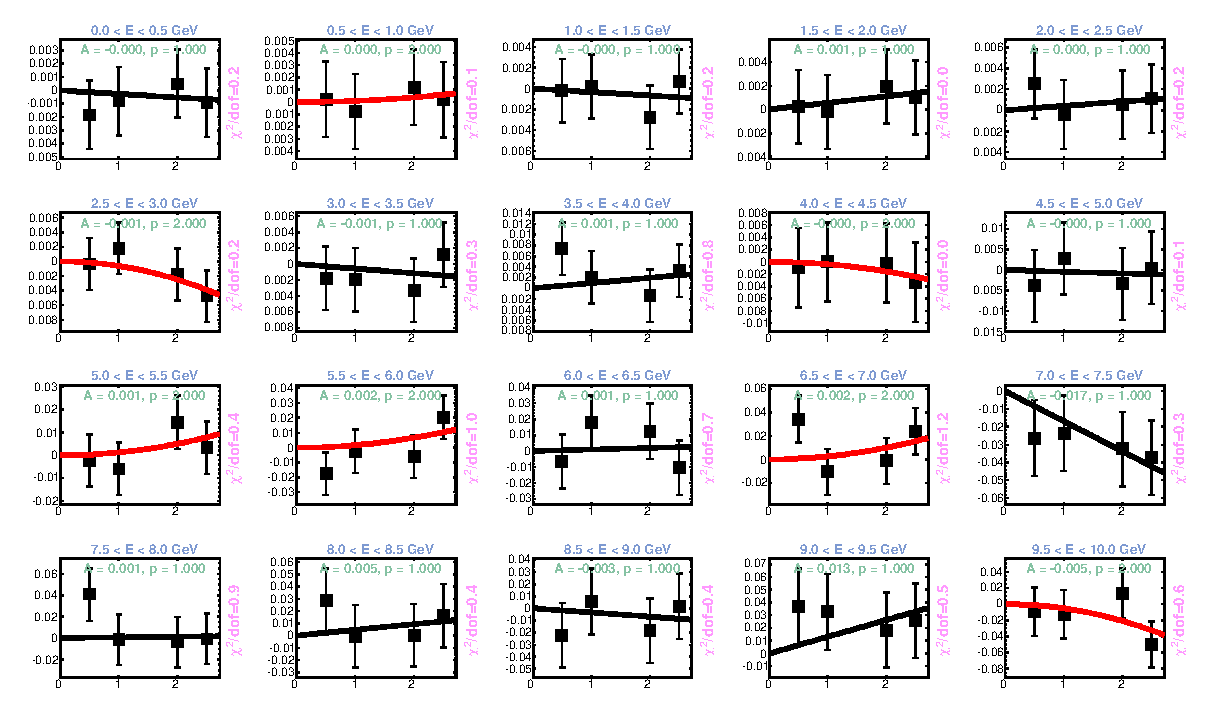
\includegraphics[width=4.0in]{figures/Horn2XOffset_nof_fits.eps}}
  \end{center}
\caption{ Fits to the near/far ratios for several values of {\bf Horn 2 Offset in $x$}. Black(Red) fit lines indicate that a linear(parabolic) fit provided the best $\chi^2$. }
\end{figure}

\begin{figure}[ht]
  \begin{center}
    {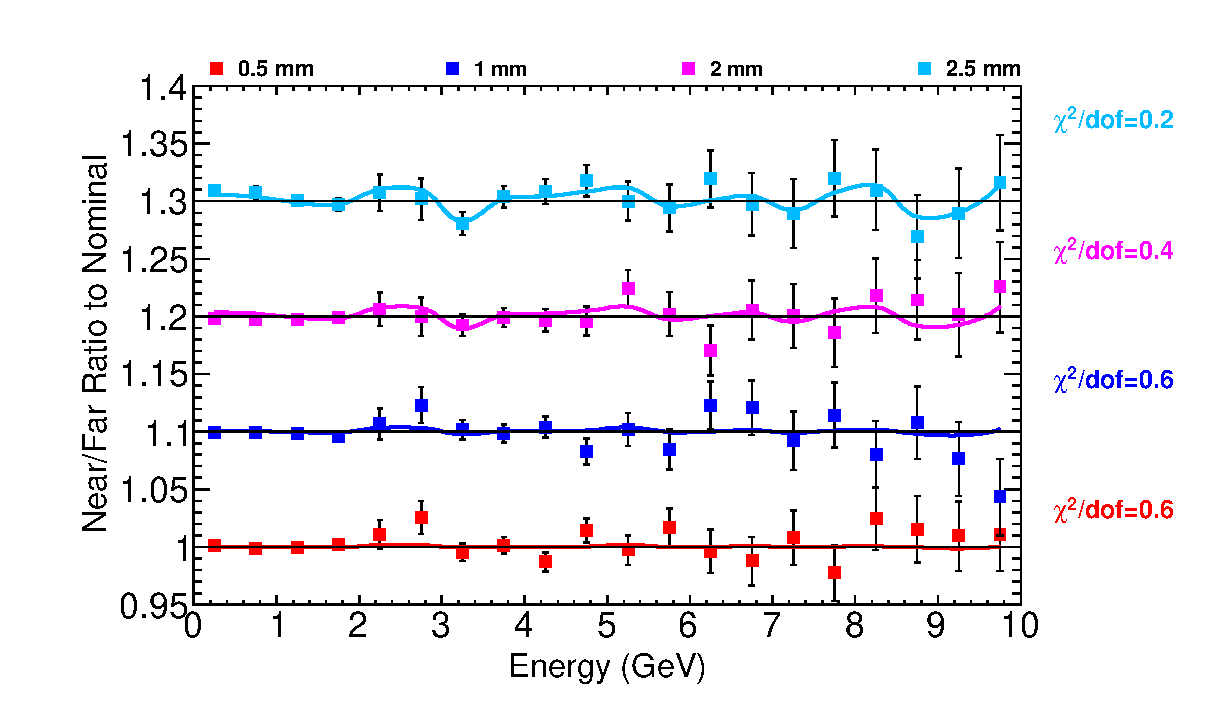
\includegraphics[width=4.0in]{figures/Horn2YOffset_nof_summary.eps}}
  \end{center}
\caption{ Near/Far double ratios to nominal for several values of {\bf Horn 2 Offset in $y$} (points) and the results of the fits to each energy bin (lines).}
\end{figure}

\begin{figure}[hb]
  \begin{center}
    {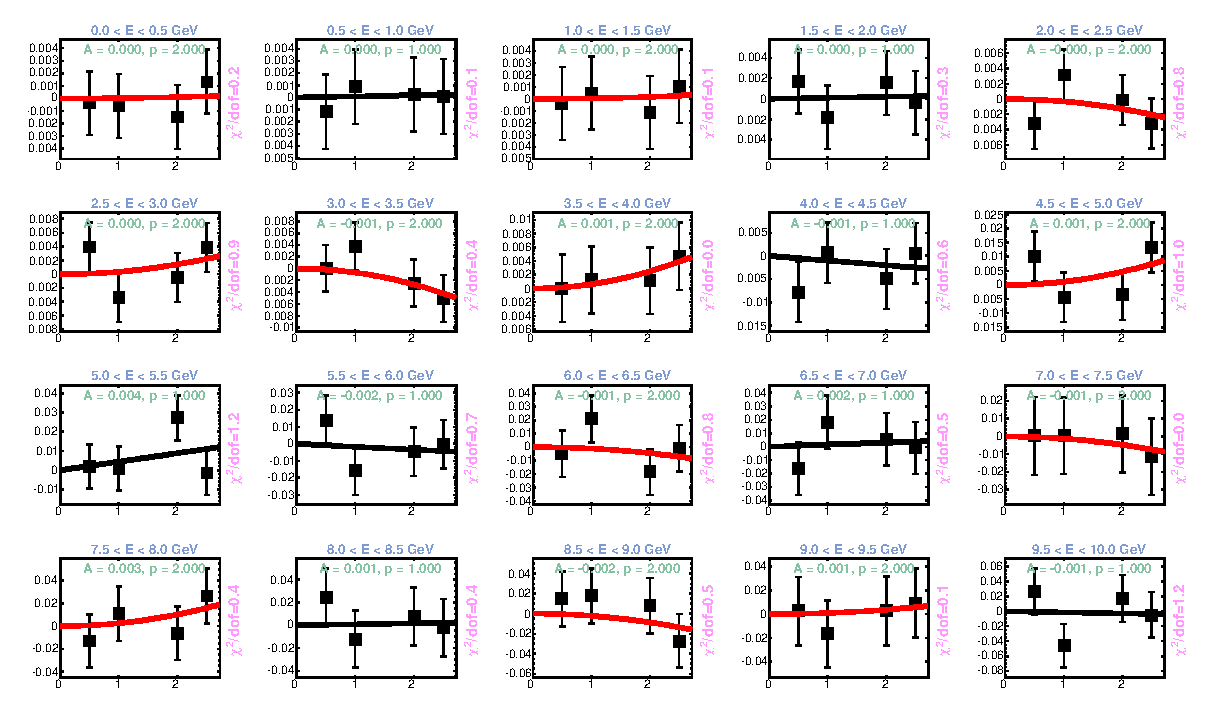
\includegraphics[width=4.0in]{figures/Horn2YOffset_nof_fits.eps}}
  \end{center}
\caption{ Fits to the near/far ratios for several values of {\bf Horn 2 Offset in $y$}. Black(Red) fit lines indicate that a linear(parabolic) fit provided the best $\chi^2$. }
\end{figure}



\begin{figure}[ht]
  \begin{center}
    {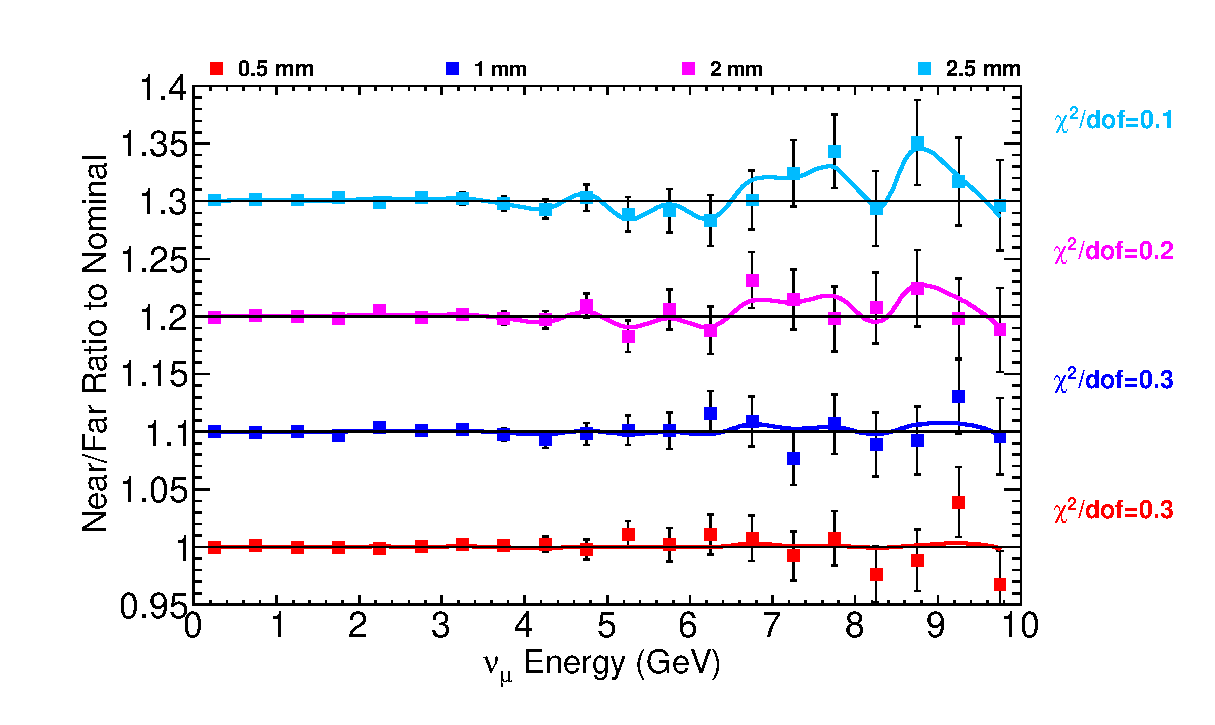
\includegraphics[width=4.0in]{figures/Horn2XTilt_nof_summary.eps}}
  \end{center}
\caption{ Near/Far double ratios to nominal for several values of {\bf Horn 2 Tilt in $x$} (points) and the results of the fits to each energy bin (lines).}
\end{figure}

\begin{figure}[hb]
  \begin{center}
    {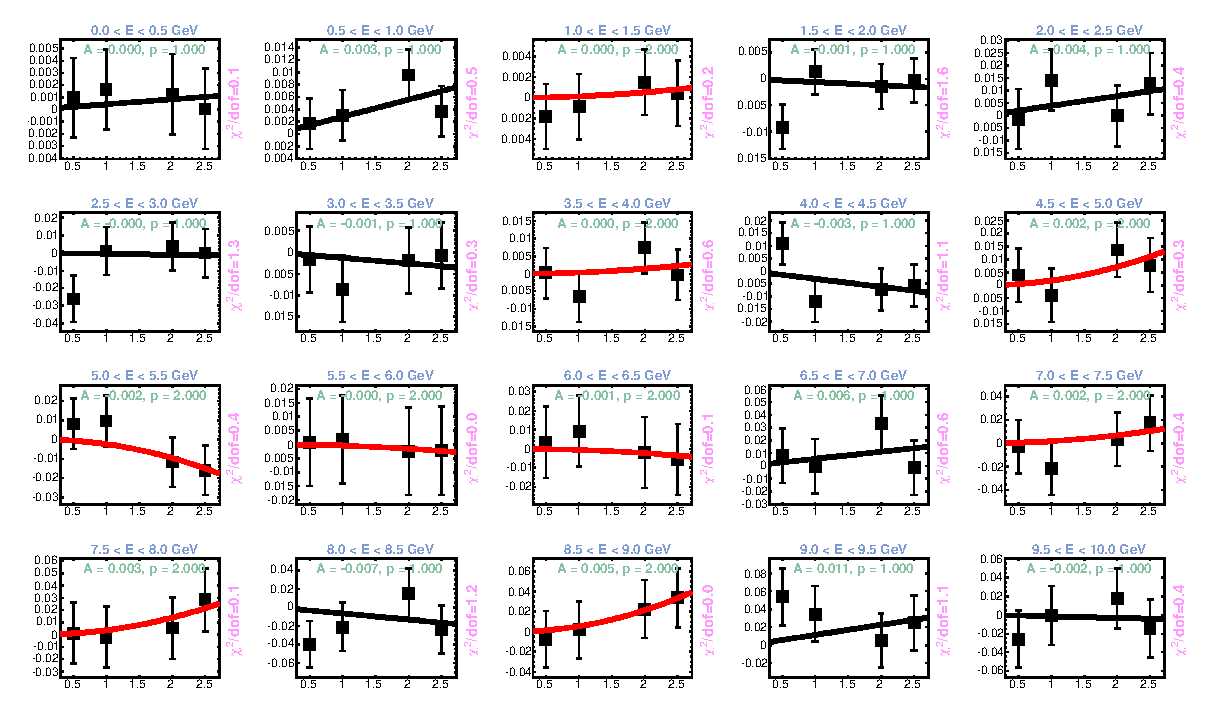
\includegraphics[width=4.0in]{figures/Horn2XTilt_nof_fits.eps}}
  \end{center}
\caption{ Fits to the near/far ratios for several values of {\bf Horn 2 Tilt in $x$}. Black(Red) fit lines indicate that a linear(parabolic) fit provided the best $\chi^2$. }
\end{figure}

\begin{figure}[ht]
  \begin{center}
    {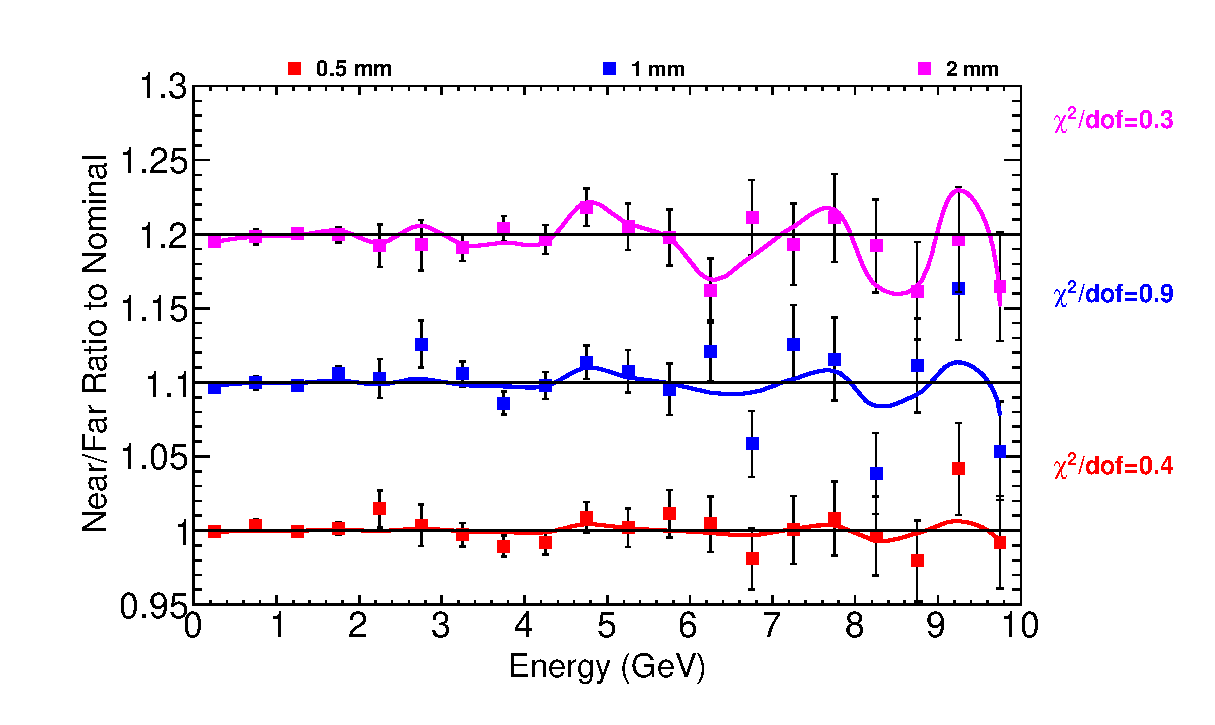
\includegraphics[width=4.0in]{figures/Horn2YTilt_nof_summary.eps}}
  \end{center}
\caption{ Near/Far double ratios to nominal for several values of {\bf Horn 2 Tilt in $y$} (points) and the results of the fits to each energy bin (lines).}
\end{figure}

\begin{figure}[hb]
  \begin{center}
    {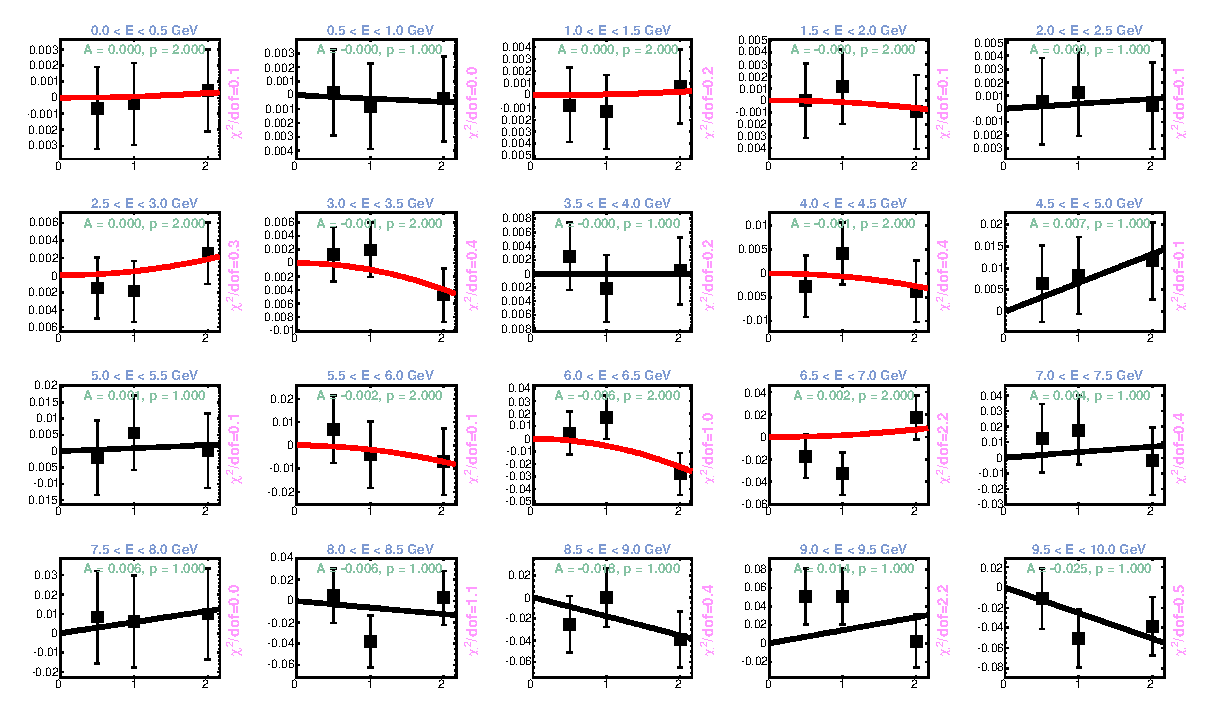
\includegraphics[width=4.0in]{figures/Horn2YTilt_nof_fits.eps}}
  \end{center}
\caption{ Fits to the near/far ratios for several values of {\bf Horn 2 Tilt in $y$}. Black(Red) fit lines indicate that a linear(parabolic) fit provided the best $\chi^2$. }
\end{figure}

\clearpage

\begin{figure}[ht]
  \begin{center}
    {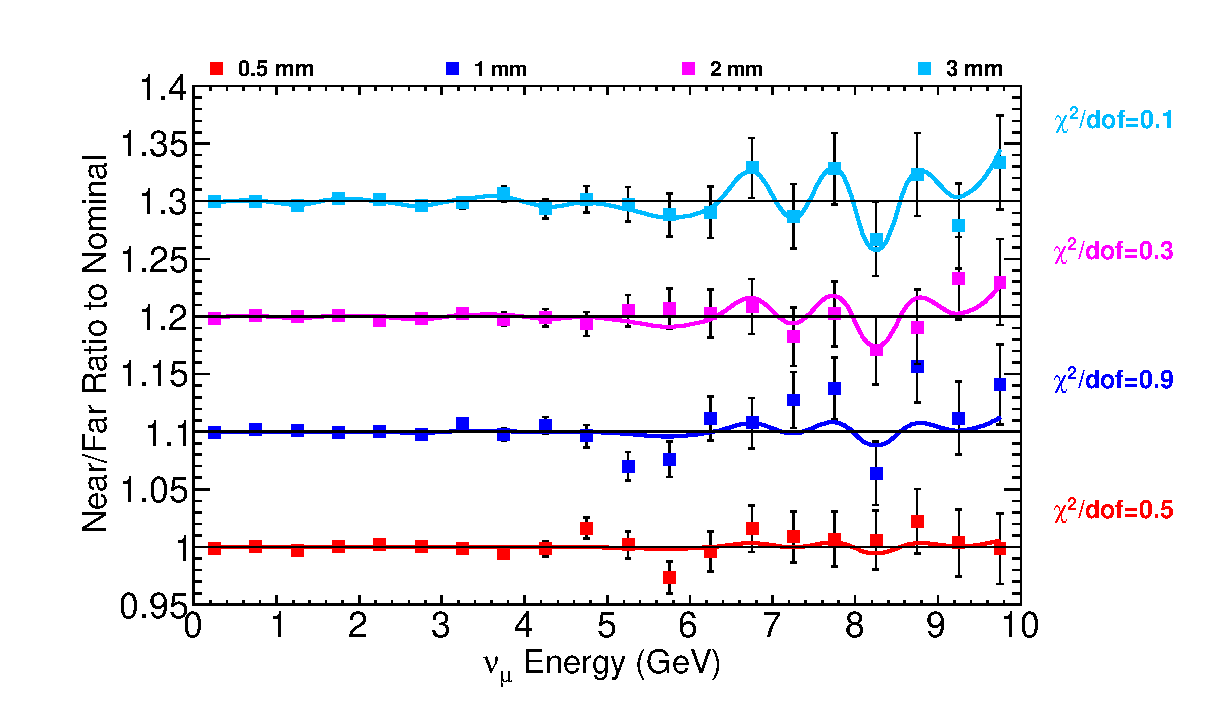
\includegraphics[width=4.0in]{figures/TargetYTilt_nof_summary.eps}}
  \end{center}
\caption{ Near/Far double ratios to nominal for several values of {\bf Target Tilt in $y$} (points) and the results of the fits to each energy bin (lines).}
\end{figure}

\begin{figure}[hb]
  \begin{center}
    {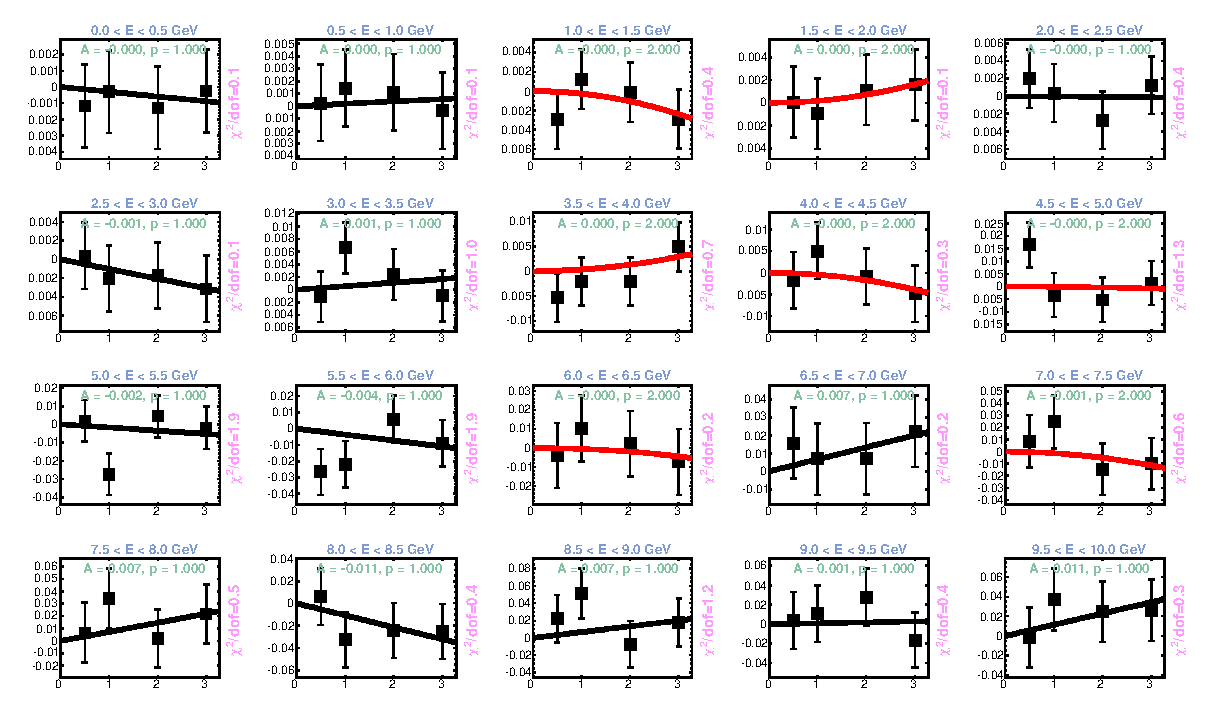
\includegraphics[width=4.0in]{figures/TargetYTilt_nof_fits.eps}}
  \end{center}
\caption{ Fits to the near/far ratios for several values of {\bf Target Tilt in $y$}. Black(Red) fit lines indicate that a linear(parabolic) fit provided the best $\chi^2$. }
\end{figure}

\clearpage
\subsection{Far Detector Position}

\begin{figure}[ht]
  \begin{center}
    {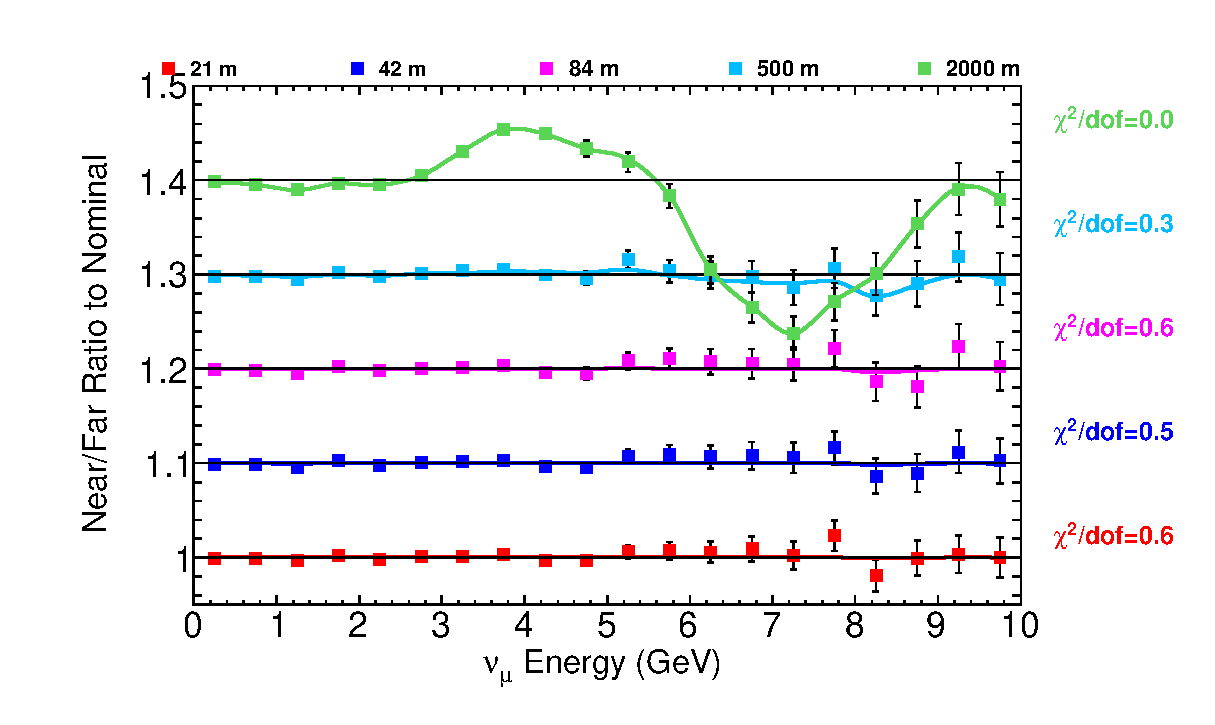
\includegraphics[width=4.0in]{figures/LBNEFDX_nof_summary.eps}}
  \end{center}
\caption{ Near/Far double ratios to nominal for several values of {\bf Far detector offset in $x$} (points) and the results of the fits to each energy bin (lines).}
\end{figure}

\begin{figure}[hb]
  \begin{center}
    {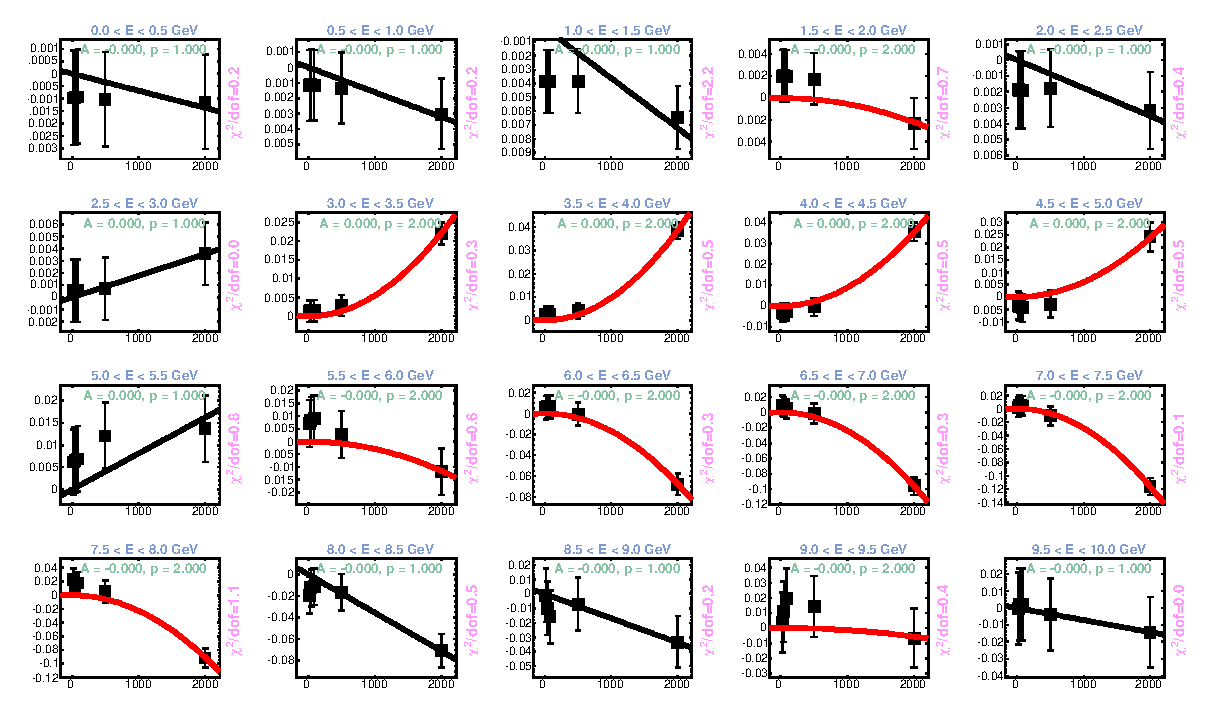
\includegraphics[width=4.0in]{figures/LBNEFDX_nof_fits.eps}}
  \end{center}
\caption{ Fits to the near/far ratios for several values of {\bf Far detector offset in $x$}. Black(Red) fit lines indicate that a linear(parabolic) fit provided the best $\chi^2$. }
\end{figure}

\begin{figure}[ht]
  \begin{center}
    {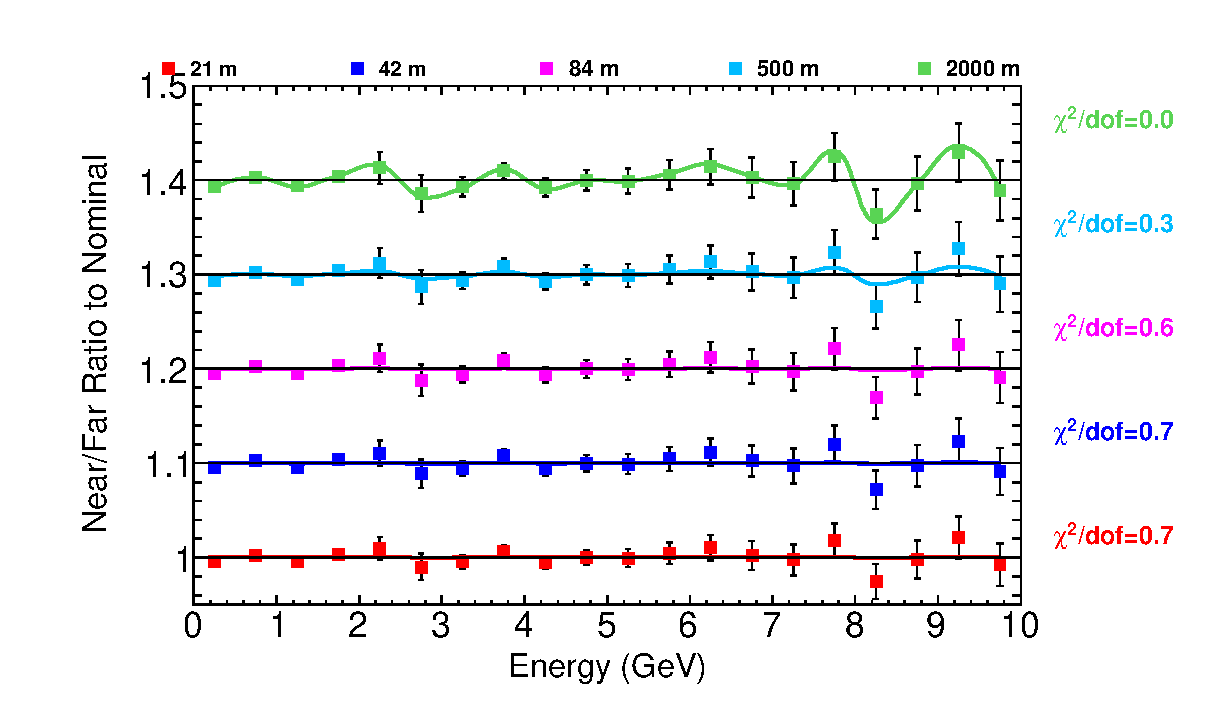
\includegraphics[width=4.0in]{figures/LBNEFDY_nof_summary.eps}}
  \end{center}
\caption{ Near/Far double ratios to nominal for several values of {\bf Far detector offset in $y$} (points) and the results of the fits to each energy bin (lines).}
\end{figure}

\begin{figure}[hb]
  \begin{center}
    {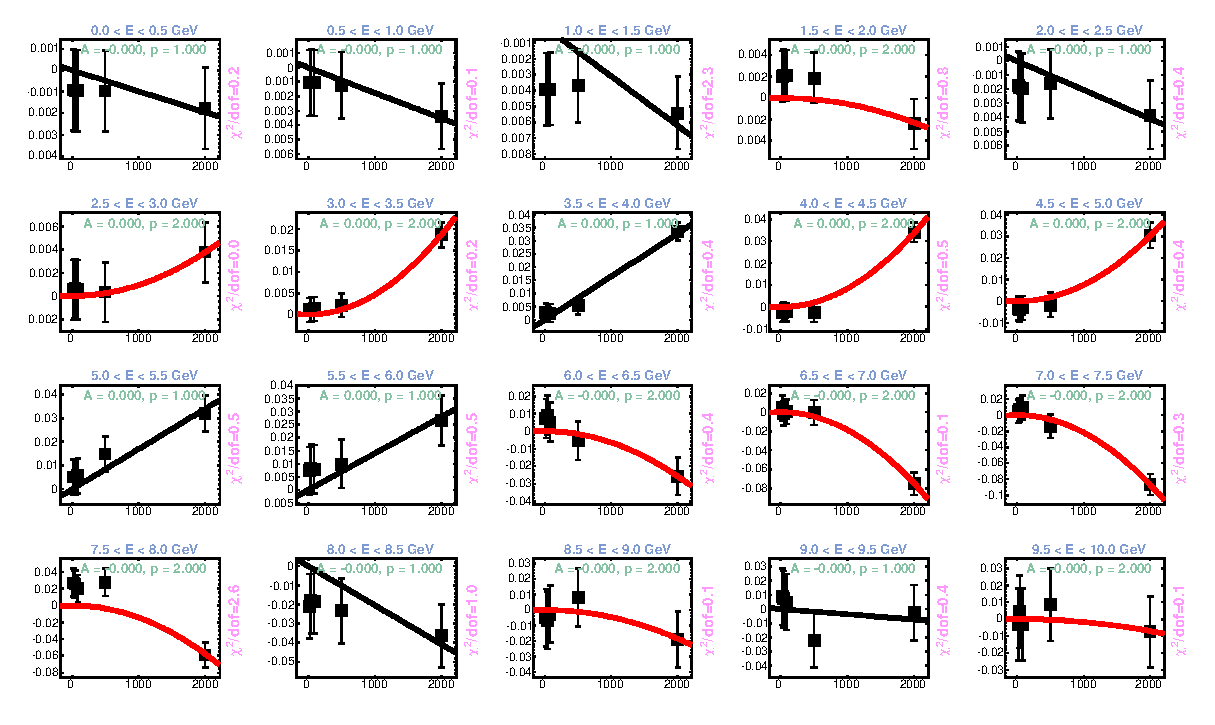
\includegraphics[width=4.0in]{figures/LBNEFDY_nof_fits.eps}}
  \end{center}
\caption{ Fits to the near/far ratios for several values of {\bf Far detector offset in $y$}. Black(Red) fit lines indicate that a linear(parabolic) fit provided the best $\chi^2$. }
\end{figure}

\clearpage
\subsection{Decay Pipe Position}

\begin{figure}[ht]
  \begin{center}
    {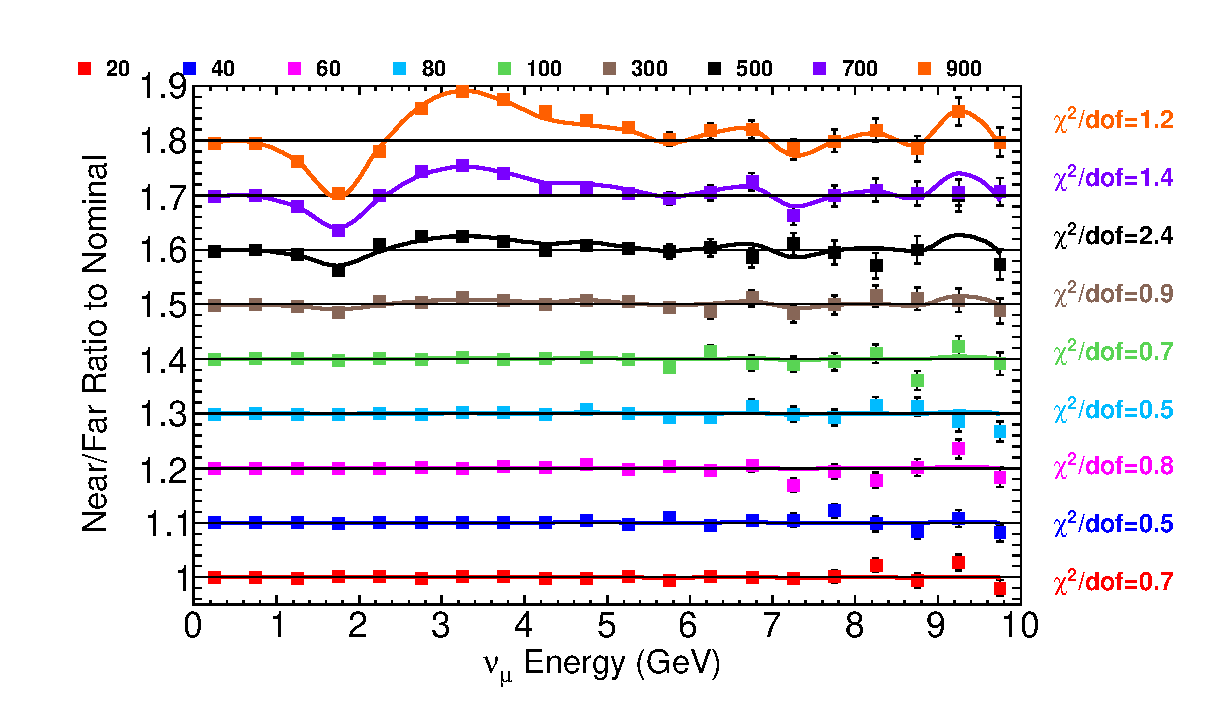
\includegraphics[width=4.0in]{figures/DecayPipeOffsetX_nof_summary.eps}}
  \end{center}
\caption{ Near/Far double ratios to nominal for several values of {\bf Decay Pipe Offset in $x$} (points) and the results of the fits to each energy bin (lines).}
\end{figure}

\begin{figure}[hb]
  \begin{center}
    {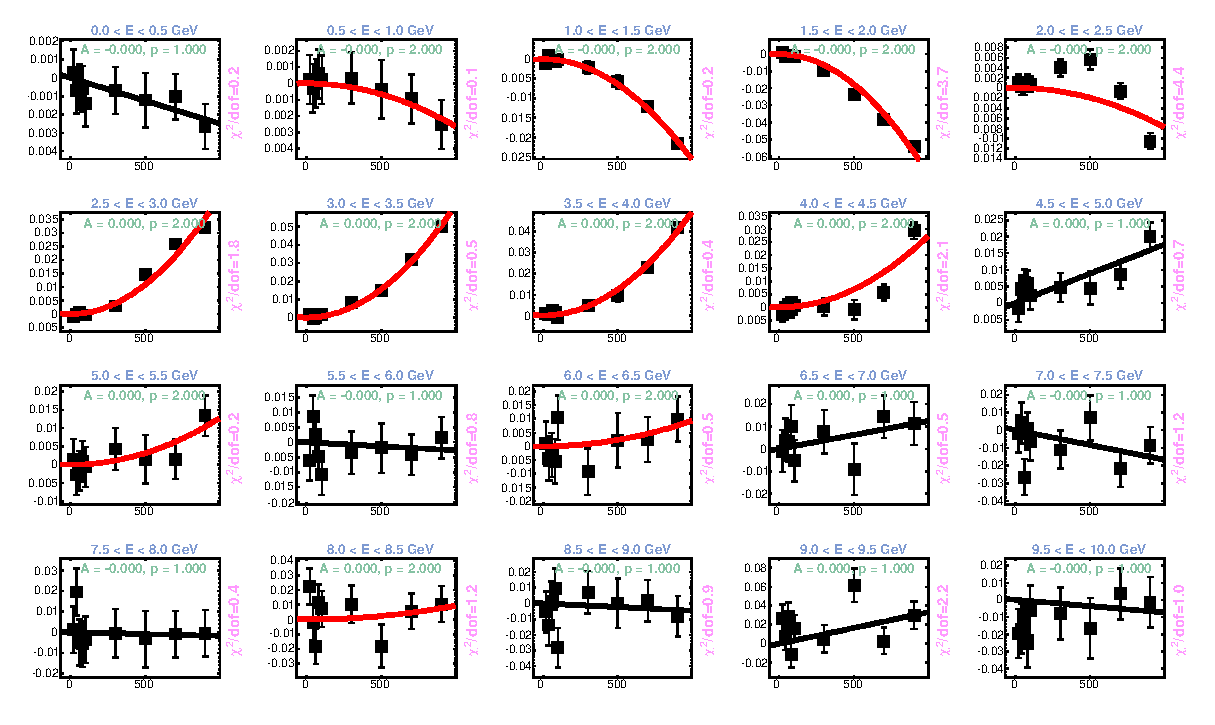
\includegraphics[width=4.0in]{figures/DecayPipeOffsetX_nof_fits.eps}}
  \end{center}
\caption{ Fits to the near/far ratios for several values of {\bf Decay Pipe Offset in $x$}. Black(Red) fit lines indicate that a linear(parabolic) fit provided the best $\chi^2$. }
\end{figure}

\clearpage
\subsection{Decay Pipe Radius}

\begin{figure}[ht]
  \begin{center}
    {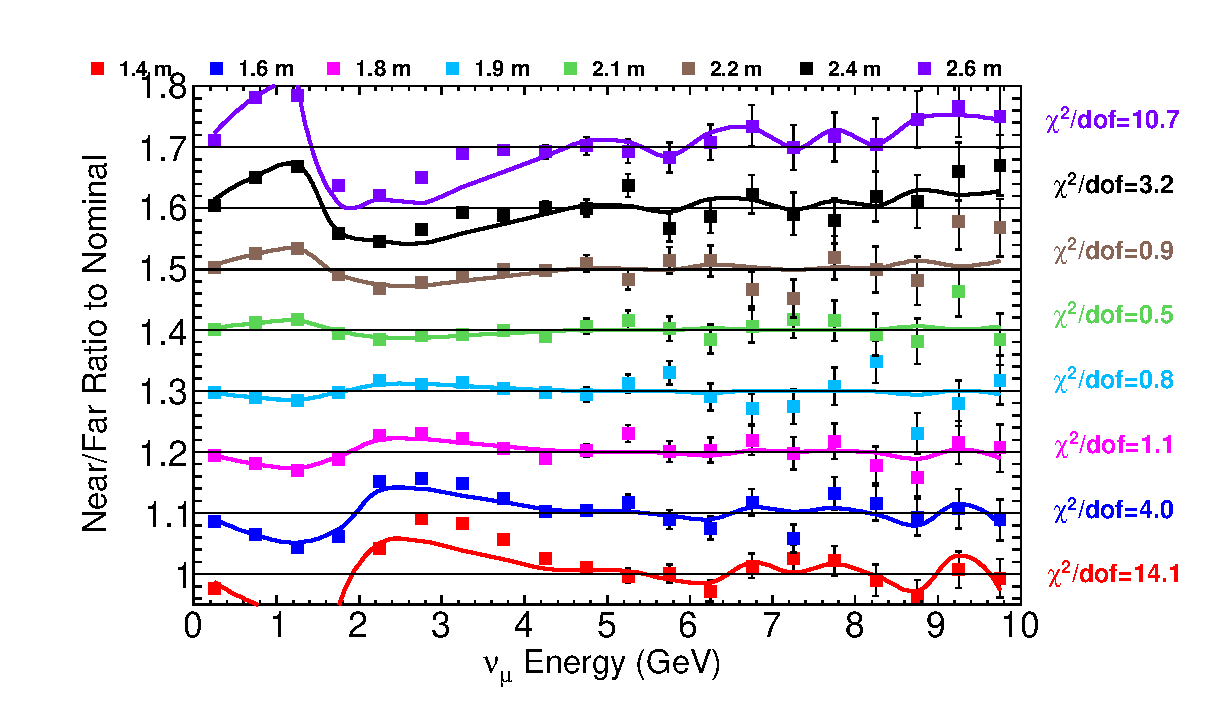
\includegraphics[width=4.0in]{figures/DecayPipeRadius_nof_summary.eps}}
  \end{center}
\caption{ Near/Far double ratios to nominal for several values of {\bf Decay Pipe Radius} (points) and the results of the fits to each energy bin (lines).}
\end{figure}

\begin{figure}[hb]
  \begin{center}
    {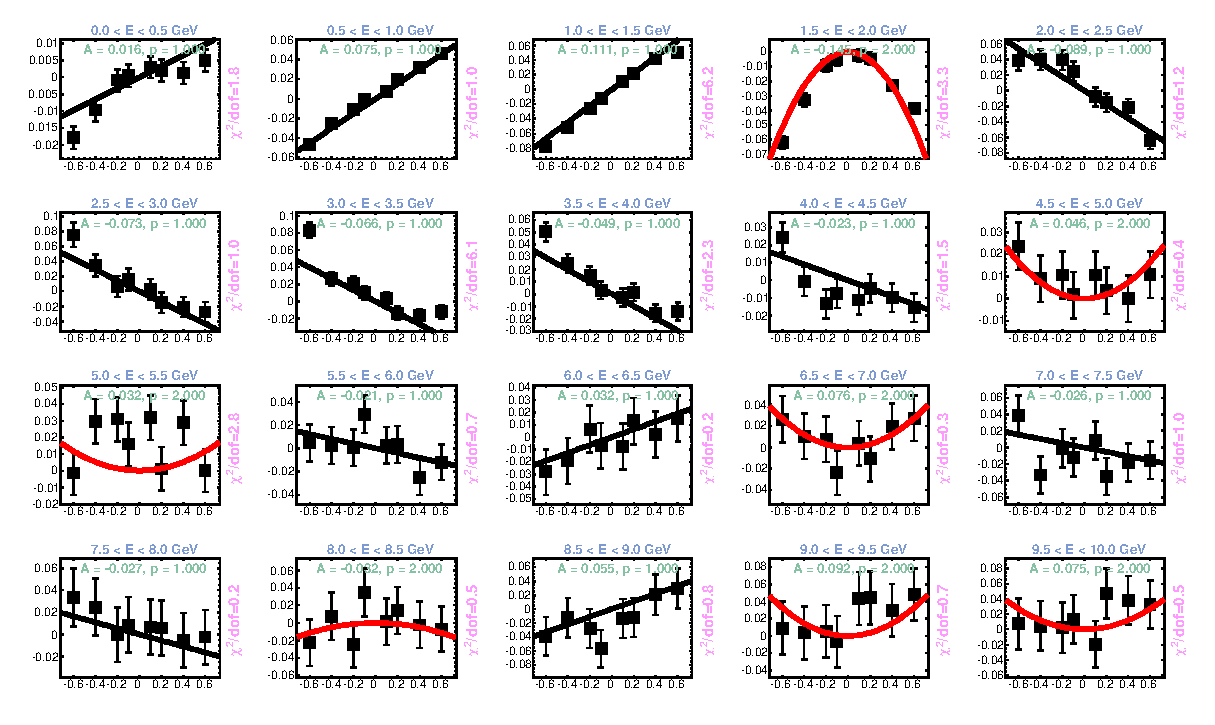
\includegraphics[width=4.0in]{figures/DecayPipeRadius_nof_fits.eps}}
  \end{center}
\caption{ Fits to the near/far ratios for several values of {\bf Decay Pipe Radius}. Black(Red) fit lines indicate that a linear(parabolic) fit provided the best $\chi^2$. }
\end{figure}

\clearpage
\subsection{Horn Current}

\begin{figure}[ht]
  \begin{center}
    {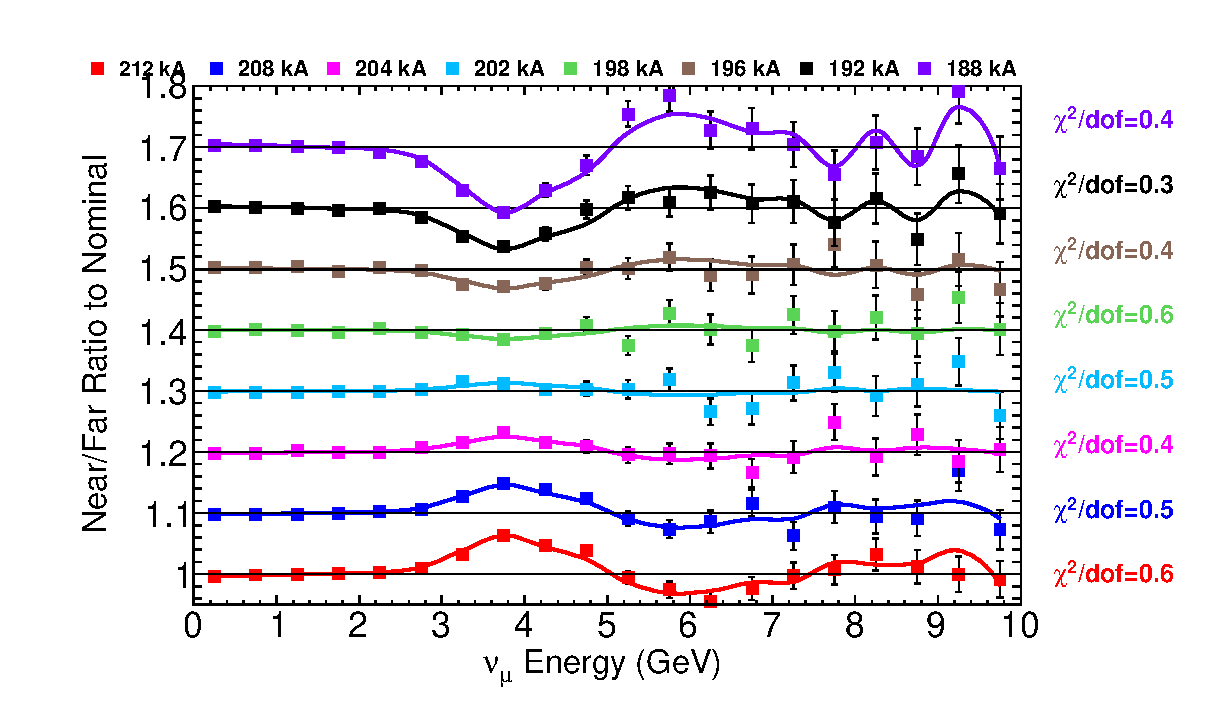
\includegraphics[width=4.0in]{figures/HornCurrent_nof_summary.eps}}
  \end{center}
\caption{ Near/Far double ratios to nominal for several values of {\bf Horn Current} (points) and the results of the fits to each energy bin (lines).}
\end{figure}

\begin{figure}[hb]
  \begin{center}
    {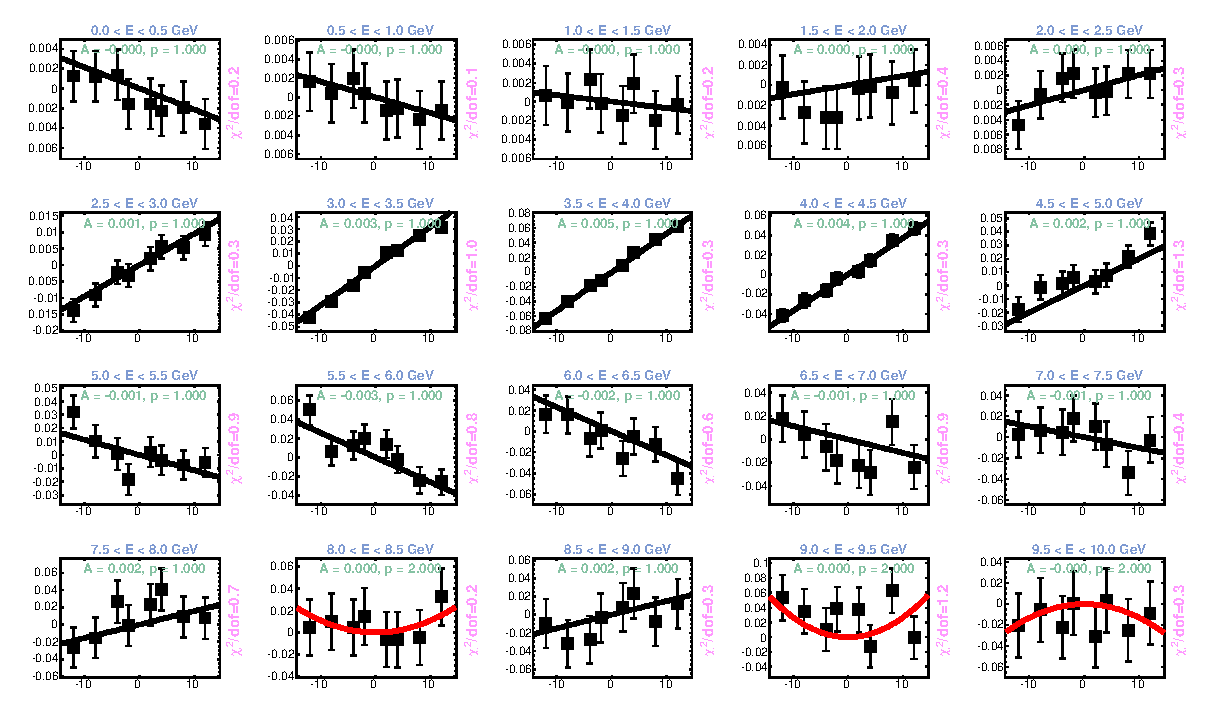
\includegraphics[width=4.0in]{figures/HornCurrent_nof_fits.eps}}
  \end{center}
\caption{ Fits to the near/far ratios for several values of {\bf HornCurrent}. Black(Red) fit lines indicate that a linear(parabolic) fit provided the best $\chi^2$. }
\end{figure}

\clearpage
\subsection{Horn Water Layer Thickness}

\begin{figure}[ht]
  \begin{center}
    {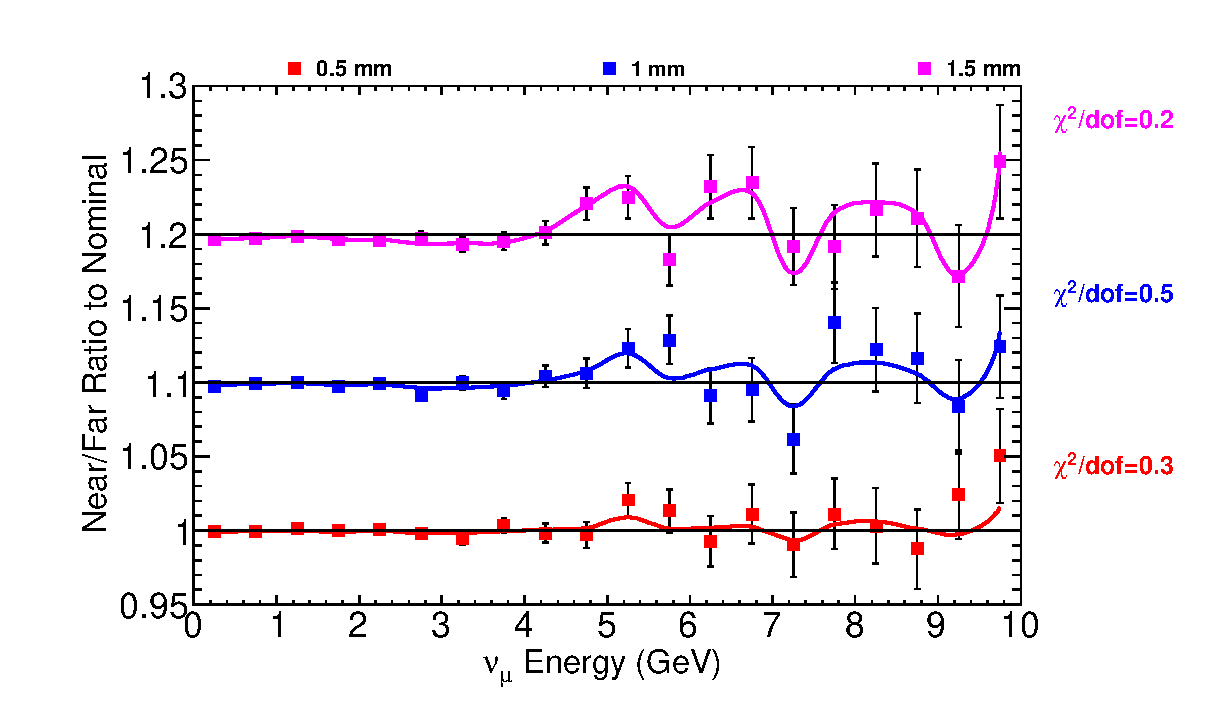
\includegraphics[width=4.0in]{figures/NominalWaterLayer__nof_summary.eps}}
  \end{center}
\caption{ Near/Far double ratios to nominal for several values of {\bf horn cooling water layer thickness} (points) and the results of the fits to each energy bin (lines).}
\end{figure}

\begin{figure}[hb]
  \begin{center}
    {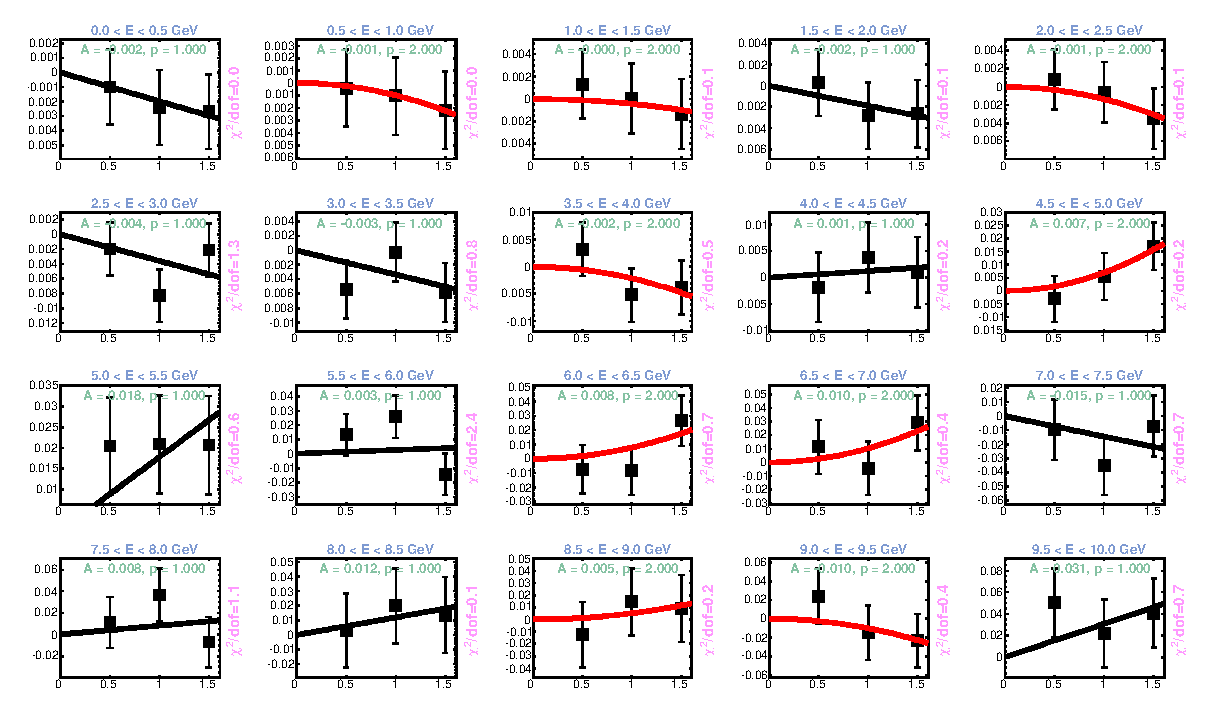
\includegraphics[width=4.0in]{figures/NominalWaterLayer__nof_fits.eps}}
  \end{center}
\caption{ Fits to the near/far ratios for several values of {\bf horn cooling water layer thickness}. Black(Red) fit lines indicate that a linear(parabolic) fit provided the best $\chi^2$. }
\end{figure}

\clearpage
\subsection{Beam size at target}

\begin{figure}[ht]
  \begin{center}
    {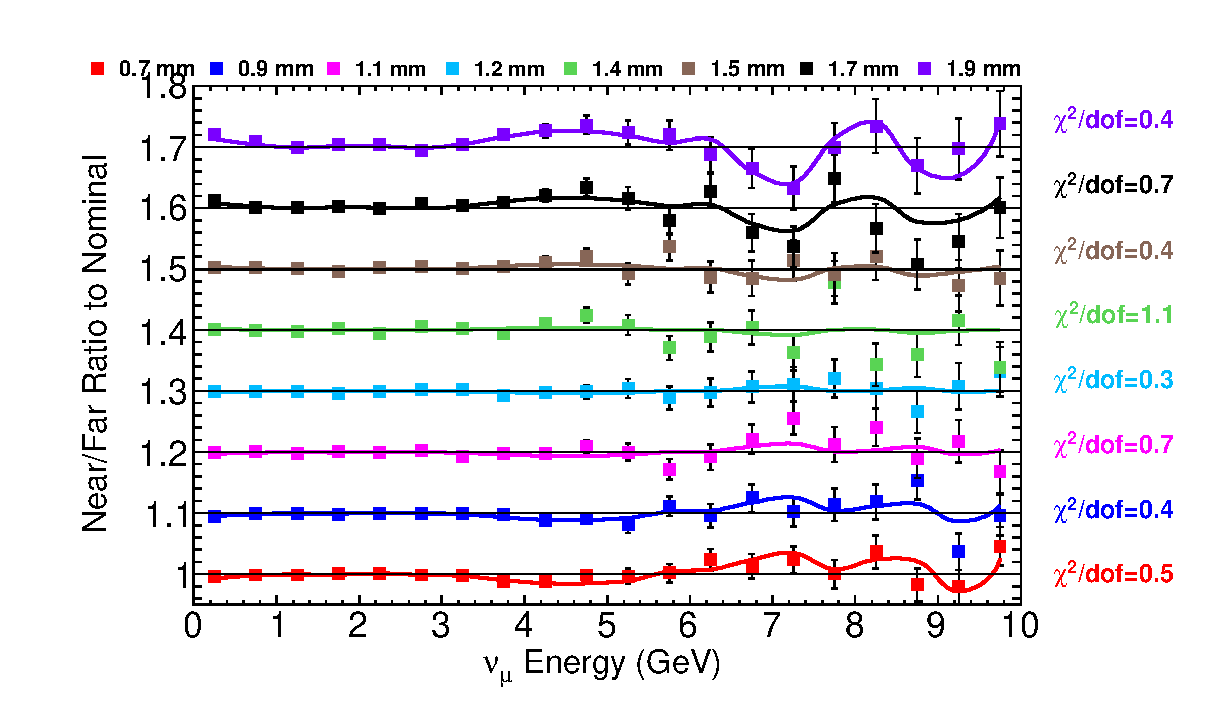
\includegraphics[width=4.0in]{figures/BeamSigmaX_nof_summary.eps}}
  \end{center}
\caption{ Near/Far double ratios to nominal for several values of {\bf Beam size in $x$} (points) and the results of the fits to each energy bin (lines).}
\end{figure}

\begin{figure}[hb]
  \begin{center}
    {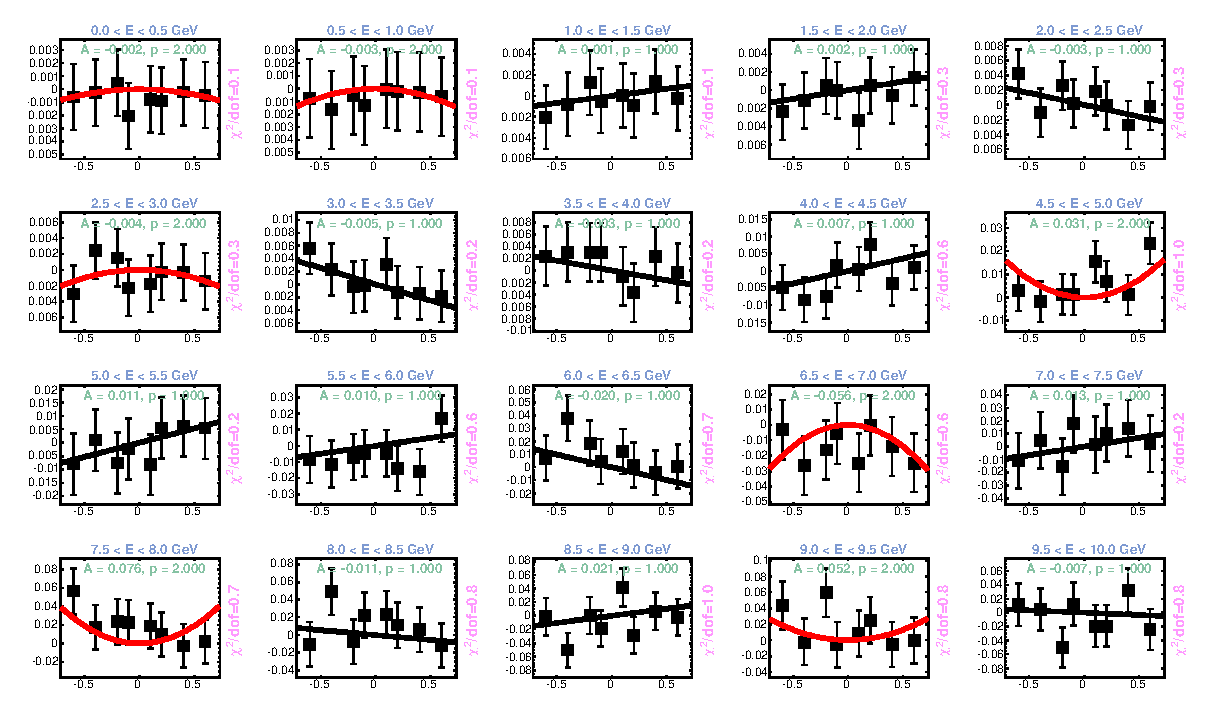
\includegraphics[width=4.0in]{figures/BeamSigmaY_nof_fits.eps}}
  \end{center}
\caption{ Fits to the near/far ratios for several values of {\bf Beam size in $x$}. Black(Red) fit lines indicate that a linear(parabolic) fit provided the best $\chi^2$. }
\end{figure}

\subsection{Beam Position at Target}

\begin{figure}[ht]
  \begin{center}
    {\includegraphics[width=4.0in]{figures/NominalX_nof_summary.eps}}
  \end{center}
\caption{ Near/Far double ratios to nominal for several values of {\bf Beam $x$ offset at target} (points) and the results of the fits to each energy bin (lines).}
\end{figure}

\begin{figure}[hb]
  \begin{center}
    {\includegraphics[width=4.0in]{figures/NominalX_nof_fits.eps}}
  \end{center}
\caption{ Fits to the near/far ratios for several values of {\bf Beam $x$ offset at target}. Black(Red) fit lines indicate that a linear(parabolic) fit provided the best $\chi^2$. }
\end{figure}

\begin{figure}[ht]
  \begin{center}
    {\includegraphics[width=4.0in]{figures/NominalY_nof_summary.eps}}
  \end{center}
\caption{ Near/Far double ratios to nominal for several values of {\bf Beam $y$ offset at target} (points) and the results of the fits to each energy bin (lines).}
\end{figure}

\begin{figure}[hb]
  \begin{center}
    {\includegraphics[width=4.0in]{figures/NominalY_nof_fits.eps}}
  \end{center}
\caption{ Fits to the near/far ratios for several values of {\bf Beam $y$ offset at target}. Black(Red) fit lines indicate that a linear(parabolic) fit provided the best $\chi^2$. }
\end{figure}

\clearpage
\subsection{Beam Angle at Target}

\begin{figure}[ht]
  \begin{center}
    {\includegraphics[width=4.0in]{figures/Tilt_t_nof_summary.eps}}
  \end{center}
\caption{ Near/Far double ratios to nominal for several values of {\bf beam tilt in $x$} (points) and the results of the fits to each energy bin (lines).}
\end{figure}

\begin{figure}[hb]
  \begin{center}
    {\includegraphics[width=4.0in]{figures/Tilt_t_nof_fits.eps}}
  \end{center}
\caption{ Fits to the near/far ratios for several values of {\bf beam tilt in $x$}. Black(Red) fit lines indicate that a linear(parabolic) fit provided the best $\chi^2$. }
\end{figure}

\clearpage
\subsection{Near Detector Position}

\begin{figure}[ht]
  \begin{center}
    {\includegraphics[width=4.0in]{figures/LBNENDX_nof_summary.eps}}
  \end{center}
\caption{ Near/Far double ratios to nominal for several values of {\bf Near detector offset in $x$} (points) and the results of the fits to each energy bin (lines).}
\end{figure}

\begin{figure}[hb]
  \begin{center}
    {\includegraphics[width=4.0in]{figures/LBNENDX_nof_fits.eps}}
  \end{center}
\caption{ Fits to the near/far ratios for several values of {\bf Near detector offset in $x$}. Black(Red) fit lines indicate that a linear(parabolic) fit provided the best $\chi^2$. }
\end{figure}

\begin{figure}[ht]
  \begin{center}
    {\includegraphics[width=4.0in]{figures/LBNENDY_nof_summary.eps}}
  \end{center}
\caption{ Near/Far double ratios to nominal for several values of {\bf Near detector offset in $y$} (points) and the results of the fits to each energy bin (lines).}
\end{figure}

\begin{figure}[hb]
  \begin{center}
    {\includegraphics[width=4.0in]{figures/LBNENDY_nof_fits.eps}}
  \end{center}
\caption{ Fits to the near/far ratios for several values of {\bf Near detector offset in $y$}. Black(Red) fit lines indicate that a linear(parabolic) fit provided the best $\chi^2$. }
\end{figure}


\clearpage
\subsection{Horn Conductor Skin Depth}

\begin{figure}[ht]
  \begin{center}
    {\includegraphics[width=4.0in]{figures/SkinDepthIC__nof_summary.eps}}
  \end{center}
\caption{ Near/Far double ratios to nominal for several values of {\bf skin depth in the horn conductors} (points) and the results of the fits to each energy bin (lines).}
\end{figure}

\begin{figure}[hb]
  \begin{center}
    {\includegraphics[width=4.0in]{figures/SkinDepthIC__nof_fits.eps}}
  \end{center}
\caption{ Fits to the near/far ratios for several values of {\bf skin depth in the horn conductors}. Black(Red) fit lines indicate that a linear(parabolic) fit provided the best $\chi^2$. }
\end{figure}

\section{Near Detector Flux Ratios and Fits}
\label{app:near_plots}

\subsection{Target Position}

\begin{figure}[ht]
  \begin{center}
    {\includegraphics[width=4.0in]{figures/TargetXOffset_near_summary.eps}}
  \end{center}
\caption{ Near detector flux ratio to nominal for several values of {\bf Target Offset in $x$} (points) and the results of the fits to each energy bin (lines).}
\end{figure}

\begin{figure}[hb]
  \begin{center}
    {\includegraphics[width=4.0in]{figures/TargetXOffset_near_fits.eps}}
  \end{center}
\caption{ Fits to the near flux ratio for several values of {\bf Target Offset in $x$}. Black(Red) fit lines indicate that a linear(parabolic) fit provided the best $\chi^2$. }
\end{figure}

\begin{figure}[ht]
  \begin{center}
    {\includegraphics[width=4.0in]{figures/TargetYOffset_near_summary.eps}}
  \end{center}
\caption{ Near detector flux ratio to nominal for several values of {\bf Target Offset in $y$} (points) and the results of the fits to each energy bin (lines).}
\end{figure}

\begin{figure}[hb]
  \begin{center}
    {\includegraphics[width=4.0in]{figures/TargetYOffset_near_fits.eps}}
  \end{center}
\caption{ Fits to the near flux ratio for several values of {\bf Target Offset in $y$}. Black(Red) fit lines indicate that a linear(parabolic) fit provided the best $\chi^2$. }
\end{figure}

\begin{figure}[ht]
  \begin{center}
    {\includegraphics[width=4.0in]{figures/TargetXTilt_near_summary.eps}}
  \end{center}
\caption{ Near detector flux ratio to nominal for several values of {\bf Target Tilt in $x$} (points) and the results of the fits to each energy bin (lines).}
\end{figure}

\begin{figure}[hb]
  \begin{center}
    {\includegraphics[width=4.0in]{figures/TargetXTilt_near_fits.eps}}
  \end{center}
\caption{ Fits to the near flux ratio for several values of {\bf Target Tilt in $x$}. Black(Red) fit lines indicate that a linear(parabolic) fit provided the best $\chi^2$. }
\end{figure}

\clearpage
\subsection{Horn 1 Position}

\begin{figure}[ht]
  \begin{center}
    {\includegraphics[width=4.0in]{figures/Horn1XOffset_near_summary.eps}}
  \end{center}
\caption{ Near detector flux ratio to nominal for several values of {\bf Horn 1 Offset in $x$} (points) and the results of the fits to each energy bin (lines).}
\end{figure}

\begin{figure}[hb]
  \begin{center}
    {\includegraphics[width=4.0in]{figures/Horn1XOffset_near_fits.eps}}
  \end{center}
\caption{ Fits to the near flux ratio for several values of {\bf Horn 1 Offset in $x$}. Black(Red) fit lines indicate that a linear(parabolic) fit provided the best $\chi^2$. }
\end{figure}

\begin{figure}[ht]
  \begin{center}
    {\includegraphics[width=4.0in]{figures/Horn1YOffset_near_summary.eps}}
  \end{center}
\caption{ Near detector flux ratio to nominal for several values of {\bf Horn 1 Offset in $y$} (points) and the results of the fits to each energy bin (lines).}
\end{figure}

\begin{figure}[hb]
  \begin{center}
    {\includegraphics[width=4.0in]{figures/Horn1YOffset_near_fits.eps}}
  \end{center}
\caption{ Fits to the near flux ratio for several values of {\bf Horn 1 Offset in $y$}. Black(Red) fit lines indicate that a linear(parabolic) fit provided the best $\chi^2$. }
\end{figure}

\begin{figure}[ht]
  \begin{center}
    {\includegraphics[width=4.0in]{figures/Horn1XTilt_near_summary.eps}}
  \end{center}
\caption{ Near detector flux ratio to nominal for several values of {\bf Horn 1 Tilt in $x$} (points) and the results of the fits to each energy bin (lines).}
\end{figure}

\begin{figure}[hb]
  \begin{center}
    {\includegraphics[width=4.0in]{figures/Horn1XTilt_near_fits.eps}}
  \end{center}
\caption{ Fits to the near flux ratio for several values of {\bf Horn 1 Tilt in $x$}. Black(Red) fit lines indicate that a linear(parabolic) fit provided the best $\chi^2$. }
\end{figure}

\begin{figure}[ht]
  \begin{center}
    {\includegraphics[width=4.0in]{figures/Horn1YTilt_near_summary.eps}}
  \end{center}
\caption{ Near detector flux ratio to nominal for several values of {\bf Horn 1 Tilt in $y$} (points) and the results of the fits to each energy bin (lines).}
\end{figure}


\begin{figure}[hb]
  \begin{center}
    {\includegraphics[width=4.0in]{figures/Horn1YTilt_near_fits.eps}}
  \end{center}
\caption{ Fits to the near flux ratio for several values of {\bf Horn 1 Tilt in $y$}. Black(Red) fit lines indicate that a linear(parabolic) fit provided the best $\chi^2$. }
\end{figure}

\clearpage
\subsection{Horn 2 Position}

\begin{figure}[ht]
  \begin{center}
    {\includegraphics[width=4.0in]{figures/Horn2XOffset_near_summary.eps}}
  \end{center}
\caption{ Near detector flux ratio to nominal for several values of {\bf Horn 2 Offset in $x$} (points) and the results of the fits to each energy bin (lines).}
\end{figure}

\begin{figure}[hb]
  \begin{center}
    {\includegraphics[width=4.0in]{figures/Horn2XOffset_near_fits.eps}}
  \end{center}
\caption{ Fits to the near flux ratio for several values of {\bf Horn 2 Offset in $x$}. Black(Red) fit lines indicate that a linear(parabolic) fit provided the best $\chi^2$. }
\end{figure}

\begin{figure}[ht]
  \begin{center}
    {\includegraphics[width=4.0in]{figures/Horn2YOffset_near_summary.eps}}
  \end{center}
\caption{ Near detector flux ratio to nominal for several values of {\bf Horn 2 Offset in $y$} (points) and the results of the fits to each energy bin (lines).}
\end{figure}

\begin{figure}[hb]
  \begin{center}
    {\includegraphics[width=4.0in]{figures/Horn2YOffset_near_fits.eps}}
  \end{center}
\caption{ Fits to the near flux ratio for several values of {\bf Horn 2 Offset in $y$}. Black(Red) fit lines indicate that a linear(parabolic) fit provided the best $\chi^2$. }
\end{figure}



\begin{figure}[ht]
  \begin{center}
    {\includegraphics[width=4.0in]{figures/Horn2XTilt_near_summary.eps}}
  \end{center}
\caption{ Near detector flux ratio to nominal for several values of {\bf Horn 2 Tilt in $x$} (points) and the results of the fits to each energy bin (lines).}
\end{figure}

\begin{figure}[hb]
  \begin{center}
    {\includegraphics[width=4.0in]{figures/Horn2XTilt_near_fits.eps}}
  \end{center}
\caption{ Fits to the near flux ratio for several values of {\bf Horn 2 Tilt in $x$}. Black(Red) fit lines indicate that a linear(parabolic) fit provided the best $\chi^2$. }
\end{figure}

\begin{figure}[ht]
  \begin{center}
    {\includegraphics[width=4.0in]{figures/Horn2YTilt_near_summary.eps}}
  \end{center}
\caption{ Near detector flux ratio to nominal for several values of {\bf Horn 2 Tilt in $y$} (points) and the results of the fits to each energy bin (lines).}
\end{figure}

\begin{figure}[hb]
  \begin{center}
    {\includegraphics[width=4.0in]{figures/Horn2YTilt_near_fits.eps}}
  \end{center}
\caption{ Fits to the near flux ratio for several values of {\bf Horn 2 Tilt in $y$}. Black(Red) fit lines indicate that a linear(parabolic) fit provided the best $\chi^2$. }
\end{figure}

\clearpage

\begin{figure}[ht]
  \begin{center}
    {\includegraphics[width=4.0in]{figures/TargetYTilt_near_summary.eps}}
  \end{center}
\caption{ Near detector flux ratio to nominal for several values of {\bf Target Tilt in $y$} (points) and the results of the fits to each energy bin (lines).}
\end{figure}

\begin{figure}[hb]
  \begin{center}
    {\includegraphics[width=4.0in]{figures/TargetYTilt_near_fits.eps}}
  \end{center}
\caption{ Fits to the near flux ratio for several values of {\bf Target Tilt in $y$}. Black(Red) fit lines indicate that a linear(parabolic) fit provided the best $\chi^2$. }
\end{figure}

\clearpage
\subsection{Far Detector Position}

\begin{figure}[ht]
  \begin{center}
    {\includegraphics[width=4.0in]{figures/LBNEFDX_near_summary.eps}}
  \end{center}
\caption{ Near detector flux ratio to nominal for several values of {\bf Far detector offset in $x$} (points) and the results of the fits to each energy bin (lines).}
\end{figure}

\begin{figure}[hb]
  \begin{center}
    {\includegraphics[width=4.0in]{figures/LBNEFDX_near_fits.eps}}
  \end{center}
\caption{ Fits to the near flux ratio for several values of {\bf Far detector offset in $x$}. Black(Red) fit lines indicate that a linear(parabolic) fit provided the best $\chi^2$. }
\end{figure}

\begin{figure}[ht]
  \begin{center}
    {\includegraphics[width=4.0in]{figures/LBNEFDY_near_summary.eps}}
  \end{center}
\caption{ Near detector flux ratio to nominal for several values of {\bf Far detector offset in $y$} (points) and the results of the fits to each energy bin (lines).}
\end{figure}

\begin{figure}[hb]
  \begin{center}
    {\includegraphics[width=4.0in]{figures/LBNEFDY_near_fits.eps}}
  \end{center}
\caption{ Fits to the near flux ratio for several values of {\bf Far detector offset in $y$}. Black(Red) fit lines indicate that a linear(parabolic) fit provided the best $\chi^2$. }
\end{figure}

\clearpage
\subsection{Decay Pipe Position}

\begin{figure}[ht]
  \begin{center}
    {\includegraphics[width=4.0in]{figures/DecayPipeOffsetX_near_summary.eps}}
  \end{center}
\caption{ Near detector flux ratio to nominal for several values of {\bf Decay Pipe Offset in $x$} (points) and the results of the fits to each energy bin (lines).}
\end{figure}

\begin{figure}[hb]
  \begin{center}
    {\includegraphics[width=4.0in]{figures/DecayPipeOffsetX_near_fits.eps}}
  \end{center}
\caption{ Fits to the near flux ratio for several values of {\bf Decay Pipe Offset in $x$}. Black(Red) fit lines indicate that a linear(parabolic) fit provided the best $\chi^2$. }
\end{figure}

\clearpage
\subsection{Decay Pipe Radius}

\begin{figure}[ht]
  \begin{center}
    {\includegraphics[width=4.0in]{figures/DecayPipeRadius_near_summary.eps}}
  \end{center}
\caption{ Near detector flux ratio to nominal for several values of {\bf Decay Pipe Radius} (points) and the results of the fits to each energy bin (lines).}
\end{figure}

\begin{figure}[hb]
  \begin{center}
    {\includegraphics[width=4.0in]{figures/DecayPipeRadius_near_fits.eps}}
  \end{center}
\caption{ Fits to the near flux ratio for several values of {\bf Decay Pipe Radius}. Black(Red) fit lines indicate that a linear(parabolic) fit provided the best $\chi^2$. }
\end{figure}

\clearpage
\subsection{Horn Current}

\begin{figure}[ht]
  \begin{center}
    {\includegraphics[width=4.0in]{figures/HornCurrent_near_summary.eps}}
  \end{center}
\caption{ Near detector flux ratio to nominal for several values of {\bf Horn Current} (points) and the results of the fits to each energy bin (lines).}
\end{figure}

\begin{figure}[hb]
  \begin{center}
    {\includegraphics[width=4.0in]{figures/HornCurrent_near_fits.eps}}
  \end{center}
\caption{ Fits to the near flux ratio for several values of {\bf HornCurrent}. Black(Red) fit lines indicate that a linear(parabolic) fit provided the best $\chi^2$. }
\end{figure}

\clearpage
\subsection{Horn Water Layer Thickness}

\begin{figure}[ht]
  \begin{center}
    {\includegraphics[width=4.0in]{figures/NominalWaterLayer__near_summary.eps}}
  \end{center}
\caption{ Near detector flux ratio to nominal for several values of {\bf horn cooling water layer thickness} (points) and the results of the fits to each energy bin (lines).}
\end{figure}

\begin{figure}[hb]
  \begin{center}
    {\includegraphics[width=4.0in]{figures/NominalWaterLayer__near_fits.eps}}
  \end{center}
\caption{ Fits to the near flux ratio for several values of {\bf horn cooling water layer thickness}. Black(Red) fit lines indicate that a linear(parabolic) fit provided the best $\chi^2$. }
\end{figure}

\clearpage
\subsection{Beam size at target}

\begin{figure}[ht]
  \begin{center}
    {\includegraphics[width=4.0in]{figures/BeamSigmaX_near_summary.eps}}
  \end{center}
\caption{ Near detector flux ratio to nominal for several values of {\bf Beam size in $x$} (points) and the results of the fits to each energy bin (lines).}
\end{figure}

\begin{figure}[hb]
  \begin{center}
    {\includegraphics[width=4.0in]{figures/BeamSigmaY_near_fits.eps}}
  \end{center}
\caption{ Fits to the near flux ratio for several values of {\bf Beam size in $x$}. Black(Red) fit lines indicate that a linear(parabolic) fit provided the best $\chi^2$. }
\end{figure}

\subsection{Beam Position at Target}

\begin{figure}[ht]
  \begin{center}
    {\includegraphics[width=4.0in]{figures/NominalX_near_summary.eps}}
  \end{center}
\caption{ Near detector flux ratio to nominal for several values of {\bf Beam $x$ offset at target} (points) and the results of the fits to each energy bin (lines).}
\end{figure}

\begin{figure}[hb]
  \begin{center}
    {\includegraphics[width=4.0in]{figures/NominalX_near_fits.eps}}
  \end{center}
\caption{ Fits to the near flux ratio for several values of {\bf Beam $x$ offset at target}. Black(Red) fit lines indicate that a linear(parabolic) fit provided the best $\chi^2$. }
\end{figure}

\begin{figure}[ht]
  \begin{center}
    {\includegraphics[width=4.0in]{figures/NominalY_near_summary.eps}}
  \end{center}
\caption{ Near detector flux ratio to nominal for several values of {\bf Beam $y$ offset at target} (points) and the results of the fits to each energy bin (lines).}
\end{figure}

\begin{figure}[hb]
  \begin{center}
    {\includegraphics[width=4.0in]{figures/NominalY_near_fits.eps}}
  \end{center}
\caption{ Fits to the near flux ratio for several values of {\bf Beam $y$ offset at target}. Black(Red) fit lines indicate that a linear(parabolic) fit provided the best $\chi^2$. }
\end{figure}

\clearpage
\subsection{Beam Angle at Target}

\begin{figure}[ht]
  \begin{center}
    {\includegraphics[width=4.0in]{figures/Tilt_t_near_summary.eps}}
  \end{center}
\caption{ Near detector flux ratio to nominal for several values of {\bf beam tilt in $x$} (points) and the results of the fits to each energy bin (lines).}
\end{figure}

\begin{figure}[hb]
  \begin{center}
    {\includegraphics[width=4.0in]{figures/Tilt_t_near_fits.eps}}
  \end{center}
\caption{ Fits to the near flux ratio for several values of {\bf beam tilt in $x$}. Black(Red) fit lines indicate that a linear(parabolic) fit provided the best $\chi^2$. }
\end{figure}

\clearpage
\subsection{Near Detector Position}

\begin{figure}[ht]
  \begin{center}
    {\includegraphics[width=4.0in]{figures/LBNENDX_near_summary.eps}}
  \end{center}
\caption{ Near detector flux ratio to nominal for several values of {\bf Near detector offset in $x$} (points) and the results of the fits to each energy bin (lines).}
\end{figure}

\begin{figure}[hb]
  \begin{center}
    {\includegraphics[width=4.0in]{figures/LBNENDX_near_fits.eps}}
  \end{center}
\caption{ Fits to the near flux ratio for several values of {\bf Near detector offset in $x$}. Black(Red) fit lines indicate that a linear(parabolic) fit provided the best $\chi^2$. }
\end{figure}

\begin{figure}[ht]
  \begin{center}
    {\includegraphics[width=4.0in]{figures/LBNENDY_near_summary.eps}}
  \end{center}
\caption{ Near detector flux ratio to nominal for several values of {\bf Near detector offset in $y$} (points) and the results of the fits to each energy bin (lines).}
\end{figure}

\begin{figure}[hb]
  \begin{center}
    {\includegraphics[width=4.0in]{figures/LBNENDY_near_fits.eps}}
  \end{center}
\caption{ Fits to the near flux ratio for several values of {\bf Near detector offset in $y$}. Black(Red) fit lines indicate that a linear(parabolic) fit provided the best $\chi^2$. }
\end{figure}


\clearpage
\subsection{Horn Conductor Skin Depth}

\begin{figure}[ht]
  \begin{center}
    {\includegraphics[width=4.0in]{figures/SkinDepthIC__near_summary.eps}}
  \end{center}
\caption{ Near detector flux ratio to nominal for several values of {\bf skin depth in the horn conductors} (points) and the results of the fits to each energy bin (lines).}
\end{figure}

\begin{figure}[hb]
  \begin{center}
    {\includegraphics[width=4.0in]{figures/SkinDepthIC__near_fits.eps}}
  \end{center}
\caption{ Fits to the near flux ratio for several values of {\bf skin depth in the horn conductors}. Black(Red) fit lines indicate that a linear(parabolic) fit provided the best $\chi^2$. }
\end{figure}

\section{Gar Detector Flux Ratios and Fits}
\label{app:far_plots}

\subsection{Target Position}

\begin{figure}[ht]
  \begin{center}
    {\includegraphics[width=4.0in]{figures/TargetXOffset_far_summary.eps}}
  \end{center}
\caption{ Far detector flux ratio to nominal for several values of {\bf Target Offset in $x$} (points) and the results of the fits to each energy bin (lines).}
\end{figure}

\begin{figure}[hb]
  \begin{center}
    {\includegraphics[width=4.0in]{figures/TargetXOffset_far_fits.eps}}
  \end{center}
\caption{ Fits to the far flux ratio for several values of {\bf Target Offset in $x$}. Black(Red) fit lines indicate that a linear(parabolic) fit provided the best $\chi^2$. }
\end{figure}

\begin{figure}[ht]
  \begin{center}
    {\includegraphics[width=4.0in]{figures/TargetYOffset_far_summary.eps}}
  \end{center}
\caption{ Far detector flux ratio to nominal for several values of {\bf Target Offset in $y$} (points) and the results of the fits to each energy bin (lines).}
\end{figure}

\begin{figure}[hb]
  \begin{center}
    {\includegraphics[width=4.0in]{figures/TargetYOffset_far_fits.eps}}
  \end{center}
\caption{ Fits to the far flux ratio for several values of {\bf Target Offset in $y$}. Black(Red) fit lines indicate that a linear(parabolic) fit provided the best $\chi^2$. }
\end{figure}

\begin{figure}[ht]
  \begin{center}
    {\includegraphics[width=4.0in]{figures/TargetXTilt_far_summary.eps}}
  \end{center}
\caption{ Far detector flux ratio to nominal for several values of {\bf Target Tilt in $x$} (points) and the results of the fits to each energy bin (lines).}
\end{figure}

\begin{figure}[hb]
  \begin{center}
    {\includegraphics[width=4.0in]{figures/TargetXTilt_far_fits.eps}}
  \end{center}
\caption{ Fits to the far flux ratio for several values of {\bf Target Tilt in $x$}. Black(Red) fit lines indicate that a linear(parabolic) fit provided the best $\chi^2$. }
\end{figure}

\clearpage
\subsection{Horn 1 Position}

\begin{figure}[ht]
  \begin{center}
    {\includegraphics[width=4.0in]{figures/Horn1XOffset_far_summary.eps}}
  \end{center}
\caption{ Far detector flux ratio to nominal for several values of {\bf Horn 1 Offset in $x$} (points) and the results of the fits to each energy bin (lines).}
\end{figure}

\begin{figure}[hb]
  \begin{center}
    {\includegraphics[width=4.0in]{figures/Horn1XOffset_far_fits.eps}}
  \end{center}
\caption{ Fits to the far flux ratio for several values of {\bf Horn 1 Offset in $x$}. Black(Red) fit lines indicate that a linear(parabolic) fit provided the best $\chi^2$. }
\end{figure}

\begin{figure}[ht]
  \begin{center}
    {\includegraphics[width=4.0in]{figures/Horn1YOffset_far_summary.eps}}
  \end{center}
\caption{ Far detector flux ratio to nominal for several values of {\bf Horn 1 Offset in $y$} (points) and the results of the fits to each energy bin (lines).}
\end{figure}

\begin{figure}[hb]
  \begin{center}
    {\includegraphics[width=4.0in]{figures/Horn1YOffset_far_fits.eps}}
  \end{center}
\caption{ Fits to the far flux ratio for several values of {\bf Horn 1 Offset in $y$}. Black(Red) fit lines indicate that a linear(parabolic) fit provided the best $\chi^2$. }
\end{figure}

\begin{figure}[ht]
  \begin{center}
    {\includegraphics[width=4.0in]{figures/Horn1XTilt_far_summary.eps}}
  \end{center}
\caption{ Far detector flux ratio to nominal for several values of {\bf Horn 1 Tilt in $x$} (points) and the results of the fits to each energy bin (lines).}
\end{figure}

\begin{figure}[hb]
  \begin{center}
    {\includegraphics[width=4.0in]{figures/Horn1XTilt_far_fits.eps}}
  \end{center}
\caption{ Fits to the far flux ratio for several values of {\bf Horn 1 Tilt in $x$}. Black(Red) fit lines indicate that a linear(parabolic) fit provided the best $\chi^2$. }
\end{figure}

\begin{figure}[ht]
  \begin{center}
    {\includegraphics[width=4.0in]{figures/Horn1YTilt_far_summary.eps}}
  \end{center}
\caption{ Far detector flux ratio to nominal for several values of {\bf Horn 1 Tilt in $y$} (points) and the results of the fits to each energy bin (lines).}
\end{figure}


\begin{figure}[hb]
  \begin{center}
    {\includegraphics[width=4.0in]{figures/Horn1YTilt_far_fits.eps}}
  \end{center}
\caption{ Fits to the far flux ratio for several values of {\bf Horn 1 Tilt in $y$}. Black(Red) fit lines indicate that a linear(parabolic) fit provided the best $\chi^2$. }
\end{figure}

\clearpage
\subsection{Horn 2 Position}

\begin{figure}[ht]
  \begin{center}
    {\includegraphics[width=4.0in]{figures/Horn2XOffset_far_summary.eps}}
  \end{center}
\caption{ Far detector flux ratio to nominal for several values of {\bf Horn 2 Offset in $x$} (points) and the results of the fits to each energy bin (lines).}
\end{figure}

\begin{figure}[hb]
  \begin{center}
    {\includegraphics[width=4.0in]{figures/Horn2XOffset_far_fits.eps}}
  \end{center}
\caption{ Fits to the far flux ratio for several values of {\bf Horn 2 Offset in $x$}. Black(Red) fit lines indicate that a linear(parabolic) fit provided the best $\chi^2$. }
\end{figure}

\begin{figure}[ht]
  \begin{center}
    {\includegraphics[width=4.0in]{figures/Horn2YOffset_far_summary.eps}}
  \end{center}
\caption{ Far detector flux ratio to nominal for several values of {\bf Horn 2 Offset in $y$} (points) and the results of the fits to each energy bin (lines).}
\end{figure}

\begin{figure}[hb]
  \begin{center}
    {\includegraphics[width=4.0in]{figures/Horn2YOffset_far_fits.eps}}
  \end{center}
\caption{ Fits to the far flux ratio for several values of {\bf Horn 2 Offset in $y$}. Black(Red) fit lines indicate that a linear(parabolic) fit provided the best $\chi^2$. }
\end{figure}



\begin{figure}[ht]
  \begin{center}
    {\includegraphics[width=4.0in]{figures/Horn2XTilt_far_summary.eps}}
  \end{center}
\caption{ Far detector flux ratio to nominal for several values of {\bf Horn 2 Tilt in $x$} (points) and the results of the fits to each energy bin (lines).}
\end{figure}

\begin{figure}[hb]
  \begin{center}
    {\includegraphics[width=4.0in]{figures/Horn2XTilt_far_fits.eps}}
  \end{center}
\caption{ Fits to the far flux ratio for several values of {\bf Horn 2 Tilt in $x$}. Black(Red) fit lines indicate that a linear(parabolic) fit provided the best $\chi^2$. }
\end{figure}

\begin{figure}[ht]
  \begin{center}
    {\includegraphics[width=4.0in]{figures/Horn2YTilt_far_summary.eps}}
  \end{center}
\caption{ Far detector flux ratio to nominal for several values of {\bf Horn 2 Tilt in $y$} (points) and the results of the fits to each energy bin (lines).}
\end{figure}

\begin{figure}[hb]
  \begin{center}
    {\includegraphics[width=4.0in]{figures/Horn2YTilt_far_fits.eps}}
  \end{center}
\caption{ Fits to the far flux ratio for several values of {\bf Horn 2 Tilt in $y$}. Black(Red) fit lines indicate that a linear(parabolic) fit provided the best $\chi^2$. }
\end{figure}

\clearpage

\begin{figure}[ht]
  \begin{center}
    {\includegraphics[width=4.0in]{figures/TargetYTilt_far_summary.eps}}
  \end{center}
\caption{ Far detector flux ratio to nominal for several values of {\bf Target Tilt in $y$} (points) and the results of the fits to each energy bin (lines).}
\end{figure}

\begin{figure}[hb]
  \begin{center}
    {\includegraphics[width=4.0in]{figures/TargetYTilt_far_fits.eps}}
  \end{center}
\caption{ Fits to the far flux ratio for several values of {\bf Target Tilt in $y$}. Black(Red) fit lines indicate that a linear(parabolic) fit provided the best $\chi^2$. }
\end{figure}

\clearpage
\subsection{Far Detector Position}

\begin{figure}[ht]
  \begin{center}
    {\includegraphics[width=4.0in]{figures/LBNEFDX_far_summary.eps}}
  \end{center}
\caption{ Far detector flux ratio to nominal for several values of {\bf Far detector offset in $x$} (points) and the results of the fits to each energy bin (lines).}
\end{figure}

\begin{figure}[hb]
  \begin{center}
    {\includegraphics[width=4.0in]{figures/LBNEFDX_far_fits.eps}}
  \end{center}
\caption{ Fits to the far flux ratio for several values of {\bf Far detector offset in $x$}. Black(Red) fit lines indicate that a linear(parabolic) fit provided the best $\chi^2$. }
\end{figure}

\begin{figure}[ht]
  \begin{center}
    {\includegraphics[width=4.0in]{figures/LBNEFDY_far_summary.eps}}
  \end{center}
\caption{ Far detector flux ratio to nominal for several values of {\bf Far detector offset in $y$} (points) and the results of the fits to each energy bin (lines).}
\end{figure}

\begin{figure}[hb]
  \begin{center}
    {\includegraphics[width=4.0in]{figures/LBNEFDY_far_fits.eps}}
  \end{center}
\caption{ Fits to the far flux ratio for several values of {\bf Far detector offset in $y$}. Black(Red) fit lines indicate that a linear(parabolic) fit provided the best $\chi^2$. }
\end{figure}

\clearpage
\subsection{Decay Pipe Position}

\begin{figure}[ht]
  \begin{center}
    {\includegraphics[width=4.0in]{figures/DecayPipeOffsetX_far_summary.eps}}
  \end{center}
\caption{ Far detector flux ratio to nominal for several values of {\bf Decay Pipe Offset in $x$} (points) and the results of the fits to each energy bin (lines).}
\end{figure}

\begin{figure}[hb]
  \begin{center}
    {\includegraphics[width=4.0in]{figures/DecayPipeOffsetX_far_fits.eps}}
  \end{center}
\caption{ Fits to the far flux ratio for several values of {\bf Decay Pipe Offset in $x$}. Black(Red) fit lines indicate that a linear(parabolic) fit provided the best $\chi^2$. }
\end{figure}

\clearpage
\subsection{Decay Pipe Radius}

\begin{figure}[ht]
  \begin{center}
    {\includegraphics[width=4.0in]{figures/DecayPipeRadius_far_summary.eps}}
  \end{center}
\caption{ Far detector flux ratio to nominal for several values of {\bf Decay Pipe Radius} (points) and the results of the fits to each energy bin (lines).}
\end{figure}

\begin{figure}[hb]
  \begin{center}
    {\includegraphics[width=4.0in]{figures/DecayPipeRadius_far_fits.eps}}
  \end{center}
\caption{ Fits to the far flux ratio for several values of {\bf Decay Pipe Radius}. Black(Red) fit lines indicate that a linear(parabolic) fit provided the best $\chi^2$. }
\end{figure}

\clearpage
\subsection{Horn Current}

\begin{figure}[ht]
  \begin{center}
    {\includegraphics[width=4.0in]{figures/HornCurrent_far_summary.eps}}
  \end{center}
\caption{ Far detector flux ratio to nominal for several values of {\bf Horn Current} (points) and the results of the fits to each energy bin (lines).}
\end{figure}

\begin{figure}[hb]
  \begin{center}
    {\includegraphics[width=4.0in]{figures/HornCurrent_far_fits.eps}}
  \end{center}
\caption{ Fits to the far flux ratio for several values of {\bf HornCurrent}. Black(Red) fit lines indicate that a linear(parabolic) fit provided the best $\chi^2$. }
\end{figure}

\clearpage
\subsection{Horn Water Layer Thickness}

\begin{figure}[ht]
  \begin{center}
    {\includegraphics[width=4.0in]{figures/NominalWaterLayer__far_summary.eps}}
  \end{center}
\caption{ Far detector flux ratio to nominal for several values of {\bf horn cooling water layer thickness} (points) and the results of the fits to each energy bin (lines).}
\end{figure}

\begin{figure}[hb]
  \begin{center}
    {\includegraphics[width=4.0in]{figures/NominalWaterLayer__far_fits.eps}}
  \end{center}
\caption{ Fits to the far flux ratio for several values of {\bf horn cooling water layer thickness}. Black(Red) fit lines indicate that a linear(parabolic) fit provided the best $\chi^2$. }
\end{figure}

\clearpage
\subsection{Beam size at target}

\begin{figure}[ht]
  \begin{center}
    {\includegraphics[width=4.0in]{figures/BeamSigmaX_far_summary.eps}}
  \end{center}
\caption{ Far detector flux ratio to nominal for several values of {\bf Beam size in $x$} (points) and the results of the fits to each energy bin (lines).}
\end{figure}

\begin{figure}[hb]
  \begin{center}
    {\includegraphics[width=4.0in]{figures/BeamSigmaY_far_fits.eps}}
  \end{center}
\caption{ Fits to the far flux ratio for several values of {\bf Beam size in $x$}. Black(Red) fit lines indicate that a linear(parabolic) fit provided the best $\chi^2$. }
\end{figure}

\subsection{Beam Position at Target}

\begin{figure}[ht]
  \begin{center}
    {\includegraphics[width=4.0in]{figures/NominalX_far_summary.eps}}
  \end{center}
\caption{ Far detector flux ratio to nominal for several values of {\bf Beam $x$ offset at target} (points) and the results of the fits to each energy bin (lines).}
\end{figure}

\begin{figure}[hb]
  \begin{center}
    {\includegraphics[width=4.0in]{figures/NominalX_far_fits.eps}}
  \end{center}
\caption{ Fits to the far flux ratio for several values of {\bf Beam $x$ offset at target}. Black(Red) fit lines indicate that a linear(parabolic) fit provided the best $\chi^2$. }
\end{figure}

\begin{figure}[ht]
  \begin{center}
    {\includegraphics[width=4.0in]{figures/NominalY_far_summary.eps}}
  \end{center}
\caption{ Far detector flux ratio to nominal for several values of {\bf Beam $y$ offset at target} (points) and the results of the fits to each energy bin (lines).}
\end{figure}

\begin{figure}[hb]
  \begin{center}
    {\includegraphics[width=4.0in]{figures/NominalY_far_fits.eps}}
  \end{center}
\caption{ Fits to the far flux ratio for several values of {\bf Beam $y$ offset at target}. Black(Red) fit lines indicate that a linear(parabolic) fit provided the best $\chi^2$. }
\end{figure}

\clearpage
\subsection{Beam Angle at Target}

\begin{figure}[ht]
  \begin{center}
    {\includegraphics[width=4.0in]{figures/Tilt_t_far_summary.eps}}
  \end{center}
\caption{ Far detector flux ratio to nominal for several values of {\bf beam tilt in $x$} (points) and the results of the fits to each energy bin (lines).}
\end{figure}

\begin{figure}[hb]
  \begin{center}
    {\includegraphics[width=4.0in]{figures/Tilt_t_far_fits.eps}}
  \end{center}
\caption{ Fits to the far flux ratio for several values of {\bf beam tilt in $x$}. Black(Red) fit lines indicate that a linear(parabolic) fit provided the best $\chi^2$. }
\end{figure}

\clearpage
\subsection{Far Detector Position}

\begin{figure}[ht]
  \begin{center}
    {\includegraphics[width=4.0in]{figures/LBNENDX_far_summary.eps}}
  \end{center}
\caption{ Far detector flux ratio to nominal for several values of {\bf Far detector offset in $x$} (points) and the results of the fits to each energy bin (lines).}
\end{figure}

\begin{figure}[hb]
  \begin{center}
    {\includegraphics[width=4.0in]{figures/LBNENDX_far_fits.eps}}
  \end{center}
\caption{ Fits to the far flux ratio for several values of {\bf Far detector offset in $x$}. Black(Red) fit lines indicate that a linear(parabolic) fit provided the best $\chi^2$. }
\end{figure}

\begin{figure}[ht]
  \begin{center}
    {\includegraphics[width=4.0in]{figures/LBNENDY_far_summary.eps}}
  \end{center}
\caption{ Far detector flux ratio to nominal for several values of {\bf Far detector offset in $y$} (points) and the results of the fits to each energy bin (lines).}
\end{figure}

\begin{figure}[hb]
  \begin{center}
    {\includegraphics[width=4.0in]{figures/LBNENDY_far_fits.eps}}
  \end{center}
\caption{ Fits to the far flux ratio for several values of {\bf Far detector offset in $y$}. Black(Red) fit lines indicate that a linear(parabolic) fit provided the best $\chi^2$. }
\end{figure}


\clearpage
\subsection{Horn Conductor Skin Depth}

\begin{figure}[ht]
  \begin{center}
    {\includegraphics[width=4.0in]{figures/SkinDepthIC__far_summary.eps}}
  \end{center}
\caption{ Far detector flux ratio to nominal for several values of {\bf skin depth in the horn conductors} (points) and the results of the fits to each energy bin (lines).}
\end{figure}

\begin{figure}[hb]
  \begin{center}
    {\includegraphics[width=4.0in]{figures/SkinDepthIC__far_fits.eps}}
  \end{center}
\caption{ Fits to the far flux ratio for several values of {\bf skin depth in the horn conductors}. Black(Red) fit lines indicate that a linear(parabolic) fit provided the best $\chi^2$. }
\end{figure}

\begin{thebibliography}{1}

\bibitem{lbnecdr} 
LBNE Conceptual Design Report Volume 2: Beamline at the Far Site.  LBNE DocDB 4317.

\bibitem{numitdh}
NuMI Technical Design Handbook, http://www-numi.fnal.gov/numwork/tdh/tdh\_index.html.
  
\bibitem{Geant4} Nuclear Instruments and Methods in Physics Research A 506 (2003) 250-303, and IEEE Transactions on Nuclear Science 53 No. 1 (2006) 270-278.\bibitem{IFIND} http://www-admscad.fnal.gov/MSDMain/cgi-bin/TPifind-web.pl 

\end{thebibliography}


\end{document}

























